\documentclass[edeposit,fullpage]{uiucthesis07} 

\usepackage[numbers,sort&compress]{natbib}
\usepackage{graphicx}
\usepackage{color}
\usepackage{subfigure}
\usepackage{tabularx}
\usepackage{amsfonts}
\usepackage{amsmath}
\usepackage{amssymb}
\usepackage[toc,page]{appendix}
\usepackage{smartdiagram}
\usesmartdiagramlibrary{additions} % library to create annotations 
\usetikzlibrary{shapes.geometric}


\renewcommand{\vec}[1]{\mathbf{#1}}
\newcommand{\Hhybtwid}{\tilde{H}_\text{hyb}}
\newcommand{\Tr}{\text{Tr}}
\newcommand{\ket}[1]{\left|#1\right\rangle}
\newcommand{\mr}[1]{\mathrm{#1}}

\bibliographystyle{apsrev}

\begin{document}

\pagenumbering{roman} \thispagestyle{empty} \begin{singlespace}

\begin{center}
\begin{Large}
%YOUR TITLE
STUDY OF CONDENSED MATTER SYSTEMS 
WITH MONTE CARLO SIMULATION
ON HETEROGENEOUS COMPUTING SYSTEMS
\end{Large}

\vspace{2.65in}

A Dissertation\\
\vspace{1.5ex}
Submitted to the Graduate Faculty of the\\
Louisiana State University and\\
Agricultural and Mechanical College\\
in partial fulfillment of the\\
requirements for the degree of\\
Doctor of Philosophy\\
\vspace{1ex}
in\\
\vspace{1ex}
The Department of Physics and Astronomy\\
\vspace{2.65in}
by\\
%Your Name\\
Sheng Feng\\
%B.S.,Institusion?, 200?\\
B.Sc., University of Science and Technology of China, 2006\\

\end{center}
\end{singlespace}
\frontmatter


\begin{dedication}
  ...
\end{dedication}

\chapter*{Acknowledgements}
\markboth{Acknowledgments}{Acknowledgments}
\addcontentsline{toc}{chapter}{Acknowledgments}

\tableofcontents 

\chapter*{Abstract}
\markboth{Abstract}{Abstract}
\addcontentsline{toc}{chapter}{Abstract}

We study the Edwards-Anderson model on a simple cubic lattice with a finite 
constant external field. We implement and optimize a code with CUDA 
architecture for efficient Monte Carlo simulation of spin glass systems on 
Graphic Processing Units. 
We study several traditional indicators, including the Binder ratio and the 
correlation length, as well as a new quantity composed of 
a ratio of susceptibilities at finite momenta.% which was recently proposed to 
%avoid the difficulties of a zero momentum quantity, for capturing the spin glass
% phase transition. 
%Unfortunately, this new indicator is fairly noisy, so 
%a large pool of samples at low temperature and small external field are 
%needed to generate results with sufficiently small statistical error for 
%analysis.  
We confirm previous findings that conventional indicators for the 
spin glass transition do not show any indication of a transition for rather 
low temperatures. 
However, the ratio of spin glass susceptibilities do show crossing behavior, 
albeit a systematic analysis is beyond the reach of the present data. 
%This calls for a more thorough study of the three dimensional Edwards-Anderson 
%model in an external field. 


One of the fundamental challenges of theoretical condensed matter physics is 
the accurate solution of quantum impurity models. By taking expansion in the 
hybridization about an exactly solved local limit, one can formulate an quantum
impurity solver. We implement the hybridization expansion quantum impurity
solver on Intel Xeon Phi accelerators, and aim to apply this approach on the
dynamic Hubbard Models.
%Dynamic Hubbard Models are proposed to reflect the fact that the wavefunction 
%of an electron in an atomic orbital expands when a second electron occupies 
%the orbital. 





\mainmatter
\chapter{General Introduction}
\section{Computer Simulations}
Computer simulation is the discipline of designing a model of an actual or 
theoretical system, executing the model on a digital computer, and 
analyzing the execution output. Computer simulations have become a useful part of mathematical modeling of 
many natural systems in various disciplines of science. 

In science, typically two types of computer simulations are used. First is a 
numerical simulation of differential equations that cannot be solved 
analytically. In the recent discovery of gravitational waves from a binary
black hole merger, LIGO scientists \cite{PhysRevLett.116.061102} used numerical simulations to provide 
estimates of the mass and spin of the final black hole, the total energy 
radiated in gravitational waves, and the peak gravitational-wave luminosity.
They were also able to verify that their observation is consistent with general 
relativity equations.

Another type is the stochastic simulation. A stochastic simulation is a 
simulation that traces the evolution of variables that can change stochastically
 (randomly) with certain probabilities. With a stochastic model, we create a 
projection which is based on a set of  random values. 
Outputs are recorded and the projection is repeated with a new 
set of random values of the variables. These steps are repeated until a 
sufficient amount of data is gathered. In the end, the distribution of the 
outputs shows the most probable estimates as well as a frame of expectations 
regarding what ranges of values the variables are more or less likely to fall 
in. 

One of the most widely used stochastic simulation methods is the Monte Carlo
methods. Named after the famous casino in Monaco, Monte Carlo methods use
repeated random sampling to obtain numerical results. By the law of large 
numbers, the average of the results obtained from a large number of trials
should be close to the expected value, and gets closer as more test trials
are performed. Therefore, an integral can be evaluated by randomly sampling
the phase space and sum over the samples. 
In physics, Monte Carlo methods are very useful for complex systems such as 
disordered systems, strongly coupled systems, etc. 

\section{Disordered Systems}
In physics, the terms order and disorder designate the presence or absence of 
translational symmetry of a system. The disorder can be put into two main categories 
according to their dynamics: annealed disorder and quenched disorder.

A system is said to present quenched disorder when 
some parameters defining its behavior are random variables which do not evolve 
with time. In these systems, the disorder is explicitly present in the Hamiltonian, 
typically under the form of random coupling $J$ among the degrees of freedom $\sigma$,
\begin{equation}
  \label{eq:4}
  H=H(\sigma,J)
\end{equation}

Spin glasses \cite{Binder-Young-1986} are a classical example of quenched disorder. 
The term spin glass was given to materials that display the lack of long-range
magnetic ordering down to zero temperature in the 1970s. 
Several families of spin glass materials have been identified. The classic examples include 
dilute metallic alloys such as CuMn with 0.9\% Mn, and concentrated insulators 
such as Eu$_x$Sr$_{1-x}$S. In these systems, the quenched disorder originates in the random dilution.
The magnetic moments in Mn and Eu can be described in term of the Heisenberg spins.
An example for real material featuring Ising-like spin is the 
LiHo$_x$Y$_{1-x}$F$_4$ insulator. Since the single-ion crystal field anisotropy
is strong compared to the magnetic interaction between Ho$^{3+}$ ions, the magnetic 
moments can be mapped on to Ising spins that only point parallel or antiparallel
to the c-axis of the tetragonal crystalline structure of the lattice. 

The discovery of the spin glass materials is due to its unique behaviors of
the susceptiblity. The now defining signature of spin glass materials is 
the cusp in the low-field ac susceptibility, first found by Cannella and Mydosh(1972).
In contrast of the usual ferromagnetic systems, this signature strongly 
suggests the lack of long range order. The physical picture of the lack 
of divergence in the susceptibility indicates a transition to a state of randomly 
frozen spins. 

In addition to the cusp, some interesting slow dynamic 
behaviors are also observed. For example, the remanent magnetization is found 
if one cools the spin glass in a field to below the transition temperature and 
turns off the field. The magnetization then decays very slowly as it approaches 
zero, signaling a very long relaxation time. Indeed, experimental spin glass
systems can never truly attain equilibrium. 

The simplest model that captures the quenched random magnetic interaction
is the Edwards-Anderson model\cite{Edwards-Anderson1975},
\begin{equation}
  \label{eq:11}
  H=-\sum_{<i,j>}J_{ij}\sigma_i\sigma_j
\end{equation}
mwhere the spins $\sigma_i=\pm 1$ are the degree of freedom, and the random coupling
$J_{ij}$ can be either Gaussian random variables, or binary random variables.

The mean-field variant of this model, the Sherrington-Kirkpatrick model\cite{Sherrington-Kirkpatrick1978,Sherrington-Kirkpatrick-1975}, was 
solved by Parisi\cite{Parisi-1980a,Parisi-1980b,Parisi1980} using the replica 
symmetry breaking approach. In this picture,m
there is a hierarchy of the replica overlap, which can be described by an untra-metric
tree. Although this theory has been accepted as the exact solution to an Edwards-Anderson
like model with infinite range interactions, its applicability in lower dimensions 
has been debated. Below the upper critical dimension ($d<6$)\cite{Harris-Lubensky-Chen-1976,Tasaki-1989,Green-Moore-Bray-1983}, 
especially at the most
physically relevant three dimensions, the nature of the spin glass phase is still not clear. 
The main competing picture is the Droplet picture, proposed by Fisher and Huse, in which 
there is only a pair of spin-flip related pure states in the thermal dynamic
limit.



A system is said to present annealed disorder when some parameters entering 
its definition are random variables, but whose evolution is related to that 
of the degrees of freedom defining the system. For example, in the case of 
structural glasses, whose Hamiltonian takes the form,
\begin{equation}
  \label{eq:12}
  H=\sum_{ij}V(r_j-r_j)
\end{equation}
where the degrees of freedom $r_i$ are the positions of the particles, and the 
function $V(r)$ is a potential. Even though there is no quenched disorder in
the Hamiltonian, at low temperature, the system stays in a frozen glassy state, 
and each particle is in a different, disordered environment.

One of the most significant differences between the two pictures is the effect 
of an external field\cite{Young-Katzgraber2004}. The droplet picture predicts that there is no phase transition
in a field, while the replica symmetry breaking picture predicts that there is a 
transition, and there is an AT line that separates the two phases. 

There have been a lot of intensive numerical studies invested in this problem over 
the last four decades. As we will explain in more detail in this thesis, numerical
simulations of spin glass system present a tremendous challenge. Obtaining the ground
state by minimization method such as branch-and-cut method is mostly useful for 
two dimensions. 

The difficulty of using minimization at three dimensions can be 
considered as consequence of the proof that the ground state energy of a three dimensional
Edwards-Anderson model is NP-complete. Therefore, the study of the three dimensional
cases is only practically feasible at finite temperatures. The best available method
is the Monte Carlo. By the very nature of spin glass systems, the long relaxation time, 
Monte Carlo simulation is bound to be very slow. This problem can be attacked from 
two directions, the advancements in algorithms and computer implementations. 
Over the last few decades, different methods to accelerate the Monte Carlo 
have been proposed and tested, we will explain more detail on these methods in this thesis. 
In addition, computer implementations have been improved to shorten the simulation
time. This is not solely on the software programming. Due to the relatively 
simple Monte Carlo method, various dedicated machines were built exclusively for the simulation
of spin glass systems. 

In the following we will review a few important milestones in the numerical study of
Edwards-Anderson model. Although the model was proposed at 1975, reliable simulations
only appear from around mid-80s.

\citet{Bhatt-Young-1985} studies used Monte Carlo simulations to study the three-dimensional
Edwards-Anderson model in zero field for samples with $3<L<20$. Results for 
$T\ge1.2$ are consistent with a conventional phase transition at $T_c=1.2$.
However, at lower temperatures, the results indicate marginal behavior. This existence
of a spin glass transition has long been considered as a open question due to the
results from this paper. 

\citet{PhysRevB.62.14237} used the parallel tempering technique to study the three dimensional
Edwards-Anderson model in helicoidal geometry. By measuring the correlation length
in the critical region,  evidence for a second order finite-temperature phase 
transition was obtained and critical exponents such as $\nu$ and $\eta$ were 
calculated. This is the beginning of a new chapter in the numerical simulation 
of spin glass. The wisdom from this paper is that the conventional indicators,
in particular the ration of cumulants of order parameter, are not sufficient 
for detecting a transition. The results from this paper bring to a universal
consensus that the spin glass transition does exist in the three dimensional
Edwards-Anderson model.

Katzgraber and Young studied the model in a magnetic field-known and 
found the absence of the de Almeida-Thouless lin. Later, a one-dimensional 
power-law diluted Ising spin-glass model has been proposed to produce an
effective model at higher dimensions\cite{Young-Katzgraber2004}. Their results for the model 
corresponding to a three-dimensional system are consistent with there being no 
de Almeida-Thouless line.

Recently, it has been suggested that the correlation length may not be a 
good indicator for the model in an external magnetic field.
The Janus collaboration \cite{Banos-2012,TheJanusCollaboration:2012:JFS:2322156.2322158} 
used their special purpose computer with FPGA to simulate
four-dimensional spin glass in a field. They studied the ratio of susceptibilities 
at the two smallest momenta, and found a crossing at finite temperature, which 
indicates that the spin glass phase can exist without time-reversal symmetry
below the upper critical dimension.


\section{Strongly Correlated Systems}
Strongly correlated materials are a wide class of compounds containing ions 
with $d-$ or $f-$orbitals, that show unusual electronic and magnetic properties. 
They include insulators, magnets, paramagnets and superconductors. In transition
metals, such as vanadium, iron, and their oxides, for example, electrons experience
strong Coulombic repulsion because of their spatial configuration, and their 
interaction cannot be described by a static mean field generated by other electrons.
\cite{RevModPhys.56.99,RevModPhys.70.1039}
The interplay of the $d$ and $f$ electrons' internal degree of freedom, such as
spin, charge and orbital moment, can exhibit many interesting ordering phenomena
at low temperatures, and makes strongly correlated systems sensitive to small
changes in external parameters such as temperature, pressure, or doping. 

The most important feature that defines these materials is that the behavior of the electrons
cannot be described in terms of non-interacting entities. Methods that work well
in weakly correlated electron materials, such as Fermi liquid theory, or Density
functional theory (DFT) \cite{RevModPhys.61.689}, are not accurate enough when applied to strongly 
correlated materials. 

Traditionally strongly correlated materials have been described using the model Hamiltonian 
approach, in which the full many-body Hamiltonian is reduced to a simpler, effective
model that retains the essence of the physical phenomena we want to understand.
One of the simplest models is the Hubbard Hamiltonian, 

\begin{equation}
  \label{eq:13}
  H=\sum_{i,j,\sigma}t_{ij}c_{i\sigma}^\dagger c_{j\sigma} + U\sum_i n_{i\uparrow} n_{i\downarrow}
\end{equation}

This Hamiltonian describes electrons with spin directions $\sigma$ moving between 
lattices $i$ and $j$, and they only interact when they meet on the same lattice 
site $i$. The kinetic term favors the delocalization of electrons, while the 
potential term favors localization, and therefore they compete against each
other. The system property is then determined by parameters such as the ratio of
the Coulomb interaction $U$ and the bandwidth $W$, the temperature $T$ and the 
hopping or number of electrons. 

One of the most popular approaches used to study the Hubbard model and other related
models is the Dynamical mean field theory (DMFT)
\cite{PhysRevB.45.6479,PhysRevLett.69.168,RevModPhys.68.13,PhysRevLett.69.1236,PhysRevLett.69.1240}. 
In DMFT, a many body lattice
problem is mapped onto a single site impurity problem with effective parameters.
DMFT has been deployed to understand the Mott transition 
\cite{PhysRevLett.69.1796,PhysRevLett.70.1666,PhysRevB.48.7167},
which has been confirmed
by experiments\cite{PhysRevLett.75.105,PhysRevB.58.3690,PhysRevLett.90.186403}. 
DMFT has also been applied to a range of other strongly correlated 
materials. With the computing power growing, and new algorithms and ideas emerging, 
one can expect much a better understanding in complicated strongly correlated 
materials.

\section{Heterogeneous Computing}
%intro
Heterogeneous computing refers to systems that use more than one kind of 
processor or cores. These systems gain performance and efficiency by adding
different processors/accelerators, and divide the task among them to utilize 
their specialized capabilities. 
Popular examples of such accelerators, according to this definition, include 
GPUs, FPGAs, Intel Xeon Phi coprocessors, etc.

%Hardwares
%FPGA?

Graphic processing units, or GPUs, are typically used in computers for image 
processing. 
Due to the performance, it is becoming increasingly common to use a general purpose 
graphics processing unit (GPGPU).
A CPU consists of a few cores optimized for sequential serial processing,
while a GPU has a massively parallel architecture 
consisting of thousands of small cores designed for handling multiple tasks 
simultaneously.
For example, a Nvidia K80 GPU \cite{nv_k80_spec} has 2496 cores, and can achieve up to 2.91 TFlops 
double precision performance and up to 8.74 TFlops single precision performance, 
and has a bandwidth of 480GB/s.
The dominant framework for GPU programming is Nvidia CUDA \cite{Nickolls:2008:SPP:1365490.1365500}, which allows 
programmers to write codes with C, C++ and Fortran and run the program on CUDA
enabled GPUs.


Intel Xeon Phi\cite{Jeffers:2013:IXP:2523262} is a coprocessor developed by Intel that features a 
X86-compatible architecture. With up to 61 cores, 244 threads, 
and 1.2 teraFLOPS of performance, a Xeon Phi delivers up to 2.3 times higher 
peak FLOPS than Intel Xeon processor E5 family-based servers.
Since languages, tools, and applications are compatible with both Intel X86 
processor and Intel Xeon Phi coprocessors, it is easier for programmers to
design, write, compile and optimize their code. 


%Pros and Cons when speeding up code within heterogeneous systems.

%Pros:
% performance

Heterogeneous systems are capable of delivering better performance than 
traditional homogeneous systems, by exploits the diversity offered by different 
processors/instruction set architectures(ISAs). 
%http://www.nvidia.com/object/why-choose-tesla.html#sthash.s2ypSuA2.dpuf
The huge performance increase over CPUs makes accelerators popular choices for
supercomputers. Tianhe-2\cite{Liao2014}, a supercomputer developed by China’s National 
University of Defense Technology, leads the list of top 500 supercomputers\cite{top500-2015-11}.
It utilizes 48,000  Intel Xeon Phi coprocessors and 32,000 Ivy Bridge-EP Xeon 
processors to achieve 33.86 petaFLOPS.

% energy efficiency
Heterogeneous systems also have much better energy efficiency. 
The power usage, as well as the cooling cost required to support the computers,
are now the primary cost of ownership for HPC data centers. Therefore,
the HPC community now understands that supercomputers should not be evaluated
solely on the basis of speed, but should also consider metrics related to 
energy efficiency. The most popular metric is the FLOPS/watt.
%[http://www.green500.org/docs/pubs/hp-pac2006.pdf]
By using energy-efficient accelerators,
heterogeneous systems can significantly reduce the energy footprint. 
In fact, heterogeneous accelerator-based systems have been dominating the 
top places of the Green500 \cite{green500},
%[www.green500.org]
a ranking of the most energy-efficient supercomputers in the world. 
In the November 2015 edition of the list\cite{green500-2015-11}, 
the top 40 supercomputers listed all used accelerators of one form or another.

%Cons:
% Complexity in programming, utilization,
Albeit the advantages in the hardware, the heterogeneous nature present new
and unique challenges for programmers and scientists. 
%Parallelism
In parallel programming, programmers need to explore the problem for 
possibility of parallelization, map the tasks onto threads, schedule for
communication and/or synchronization, and solve problems such as race conditions,
etc. Communication and barriers could result in parallel slow-down, 
a situation in which the overhead from communication outweighs the performance 
gain from parallelism, and further parallelization increases the time to finish
the workload. 
Accelerators use a huge number of cores to achieve great performance. 
To utilize all the cores, a lot of parallelisms is required, and efficient 
parallelism is critical. 

%memory architecture
Different processors/accelerators often feature different memory architecture.
To achieve the best possible performance, architecture aware memory access is 
very important to utilize the high memory bandwidth and reduce the latency.
This is even more important in programming for accelerators such as GPUs than in
CPU programming, since the latency is not hidden by large cache.
For example, in CUDA %, the architecture Nvidia use for programming their GPUs, 
there are different types of memory such as registers, local memory, shared 
memory, global memory, and constant memory, etc. Each of these types is 
different in terms of size, latency, bandwidth, and performance profile for 
various access modes, and one have to make conscious decisions when using them
in order to avoid performance penalties and make the best of the hardware. 
In CUDA, this means programmers need to put the correct qualifiers in front when 
declaring their variables, and move their variables around the memory hierarchy 
when needed.
 
%Communication
%Since the accelerators are usually connected to the CPU via the PCI express bus,their communication bandwidth with the CPU are limited.
%CPU-accelerator communication
%Inter-accelerator communication

% Portability, compilers and tools
The different architecture of processors makes it hard to write portable codes.
First, some programming languages, such as CUDA, and associated compilers and tools,
 are exclusive for their specific platforms. In order to program, debug, profile 
and optimize a code for different platforms, programmers often need to understand 
more than one set of tools. 
Second, different performance profile for different hardwares are very
different from each other, thus an efficient code on one platform may not be
optimal for another. 
Fortunately, tools that aim at portable accelerated codes with great performance, such as 
OpenMP\cite{dagum1998openmp}, OpenCL\cite{Stone:2010:OPP:622179.1803953} and OpenACC\cite{OpenACC}, are evolving along with the hardware, and they allow programmers
to worry more about the problem rather than the language and hardware they are
using, and make it much easier to develop and maintain codes that run on heterogeneous systems.




%Programming models

\section{Scope and Structure}
In this dissertation, I cover my work in two projects.

The first is the work on the Three-Dimensional Edwards-Anderson Model in an External
field. We first discuss the model and the theoretical understanding in chapter 
\ref{chap:SGintro}. Then, an efficient GPU implementation is described in chapter
\ref{chap:SG_imp}. We show the results obtained from this study in chapter \ref{chap:sg_result}.
Some additional research using the covariance matrix is covered in the appendix.

Second, we show our work on a Continuous Time Quantum Monte Carlo solver implemented
on the Intel Xeon Phi platform in chapter \ref{chap:cthyb}. We first discuss the 
motivation and formalism behind this implementation. Then, we show the detail of
the implementation and the optimization. We also included some preliminary benchmarking
results.



%%% Local Variables:
%%% mode: latex
%%% TeX-master: "../thesis"
%%% End:

\chapter{Spin Glass}
\label{chap:SGintro}
\section{Introduction and Experimental Features}
\label{sec:sg_intro}
Spin glasses \cite{Binder-Young-1986} are magnetic systems where the frozen-in quenched  
disorder leads to conflicting couplings among magnetic moments, which prevents the formation 
of long-range magnetic ordering, e.g.,ferromagnetic ordering.

The prototype material is a dilute magnetic alloy, with a small amount of 
magnetic impurity (such as Fe, Mn) randomly substituted into the lattice of a 
noble metallic host (i.e. Cu, Au). On the other hand, insulators such as 
Eu$_x$Sr$_{1-x}$S, and LiHo$_{x}$Y$_{1-x}$F$_{4}$ also show spin glass behavior.
 
The physics underlying the spin glass behavior comes from the quenched 
randomness: a pair of spins has a roughly equal a priori probability of having
a ferromagnetic or an anti-ferromagnetic interaction. For the dilute magnetic 
alloy, the conduction electron-mediated 
Ruderman-Kittel-Kasuya-Yosida (RKKY) interactions between the localized moments
 oscillates strongly with distance, 
 \begin{equation}
   \label{eq:RKKY}
   J(R)=J_0\frac{\cos(2k_FR+\phi_0)}{(k_FR)^3}, R\rightarrow 0
 \end{equation}
Here $J_0$ and $\phi_0$ are constants, and $k_F$ is the Fermi wave number of the
host metal. Since the distance between any pair of spins is random, some of the $R$
will be positive, some will be negative,
thus forming ferromagnetic/antiferromagnetic bonds randomly, and no spin 
alignment would satisfactory all exchange bonds. In the other words, the 
ground state energy cannot be obtained by minimizing the local energy 
of every pair of spins.

\begin{figure}[!h]
  \label{fig:rkky}
  \centering
  \includegraphics[width=0.5\textwidth]{img/RKKY.png}
  \caption{Sketch of RKKY interaction.}
\end{figure}

Experiments demonstrated many unusual features of spin glass materials.

\subsection{AC susceptibility}
The experimental observation of a sharp cusp in the AC susceptibility, first
carried out on a metallic AuFe by \citet{PhysRevB.6.4220}, as shown in as shown in Fig.\ref{fig:au-fe-cusp}, 
sparked the research on spin glass materials. 
%Similar cusps in low-field AC susceptibility also occur in other diluted 
%magnetic alloys such as CuMn, AgMn, AuMn, and AuCr.
\citet{THOLENCE1977875,:/content/aip/proceeding/aipcp/10.1063/1.30603,
:/content/aip/proceeding/aipcp/10.1063/1.30565} also found similar cusp occurring in PtMn alloys.
Upon applying a magnetic field, Cannella and Mydosh also found that even a weak
magnetic field strongly rounds the cusp of $\chi(T)$.

The AC susceptibility of spin glass also features pronounced frequency dependence. 
In figure \ref{fig:ac-chi-freq}, we show the AC susceptibility of CuMn for various
AC frequencies $\nu$ ranging from 10 Hz to 10,000 Hz. As shown in the figure, the
peak of $\chi(T)$ gradually shift to lower temperature with decreased $\nu$.
This is natural considering that as one probes the spin motion at longer time scales,
the slowing down and freezing of the spins tends to occur at lower temperatures.

\begin{figure}
  \centering
  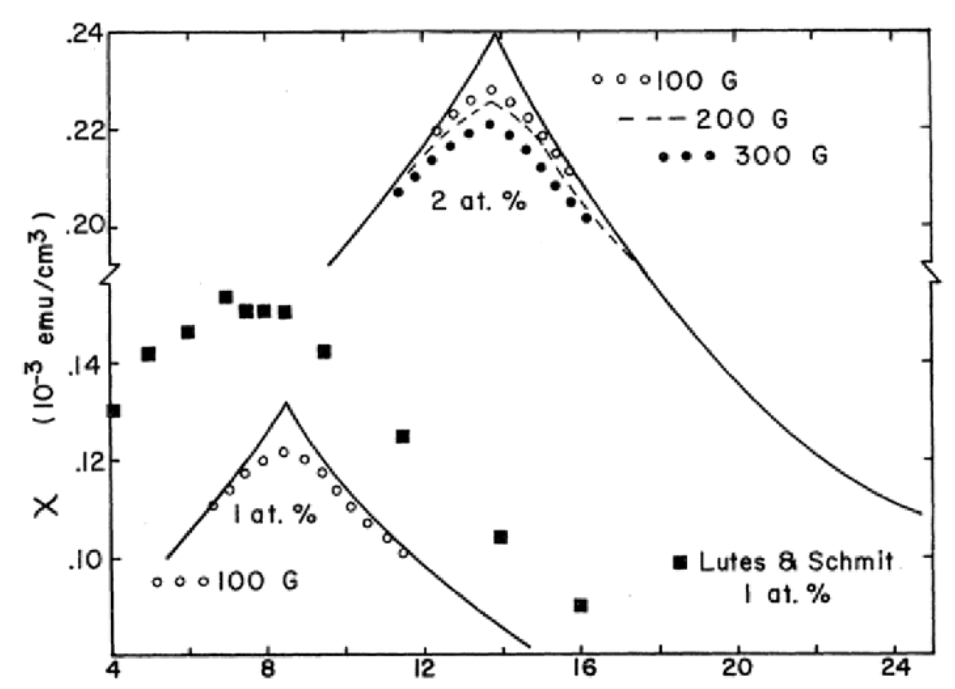
\includegraphics[width=0.6\textwidth]{img/cusp.png}
  \caption{\label{fig:au-fe-cusp}Susceptibility of Au-Fe alloys ploted vs. temperature. Full curves refer to zero field, from \citet{PhysRevB.6.4220}.}
\end{figure}
\begin{figure}
  \centering
  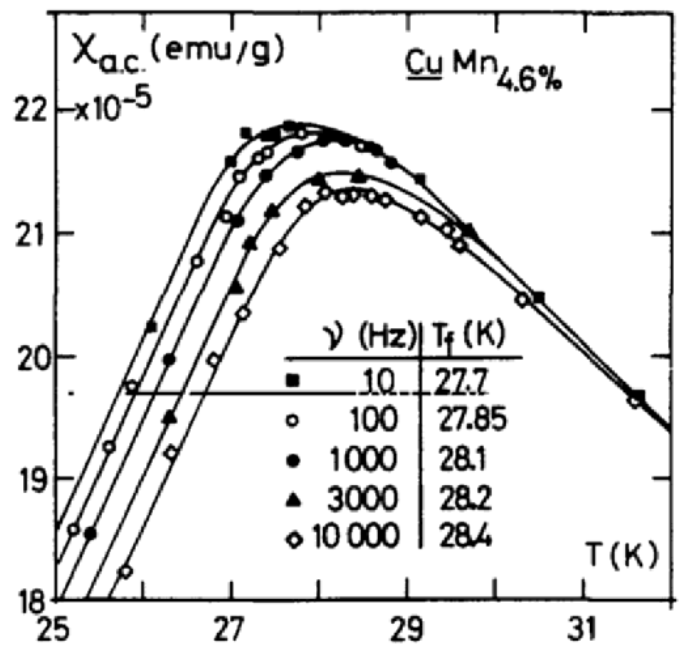
\includegraphics[width=0.5\textwidth]{img/ac-chi-freq.png}
  \caption{\label{fig:ac-chi-freq}The AC susceptibility of CuMn with 4.6\% Mn plotted vs temperature, for various ac frequencies, from \citet{THOLENCE1980113}.}
\end{figure}


\subsection{Remanent Magnetization}
The magnetization process of spin glass is characterized by strong remanence effects.
Figure \ref{fig:trm-irm} shows remanent magnetization of AuMn measured in two ways:
the thermoremanent magnetization is measured by cooling the sample in a field $H$ 
from above $T_g$ to $T<T_g$, and removing the field afterward; the isothermal 
remanent magnetization is measured by first cooling down the sample in zero field to
below $T_g$, then applying a field and removing it. At lower fields, there is a 
clear difference between the two cases. Upon increasing $H$, the TRM increases to 
a maximum and the decrease, while the IRM shows a monotonic increase. With a large
magnetic field, both TRM and IRM saturate and agree. 


A particularly interesting feature of this irreversible behavior in spin glasses 
is the slow decay of the various remanent magnetizations with time. 
Relaxation phenomena occur below Tc on a typical timescale of 1 sec -- 1hr
\cite{tholence:jpa-00215633,Holtzberg1977,NIEUWENHUYS1977880}. This relaxation is distinctly non-exponential. It can be 
described in terms of power-laws\cite{NIEUWENHUYS1977880} or even, at not too late stages, by a 
logarithmic behavior\cite{Holtzberg1977} (see figure \ref{fig:au-fe-remanent}).

%including the cusp instead of a true divergence in the low-field, low-frequency 
%susceptibility and the discrepancy of magnetic response between zero-field and field cooling 
%measurements, as shown in Fig \ref{fig:experimentsSG}. 

\begin{figure}
  \centering
  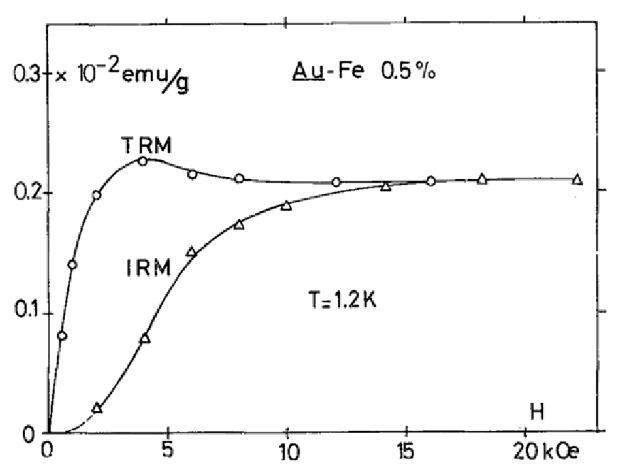
\includegraphics[width=0.6\textwidth]{img/trm-irm.png}
  \caption{\label{fig:trm-irm}The isothermal remanent magnetization (IRM) and 
thermoremanent magnetization (TRM) of AuMn with 0.5\% Mn vs magnetic field, 
from \citet{tholence:jpa-00215633}.}
\end{figure}

\begin{figure}
  \centering
  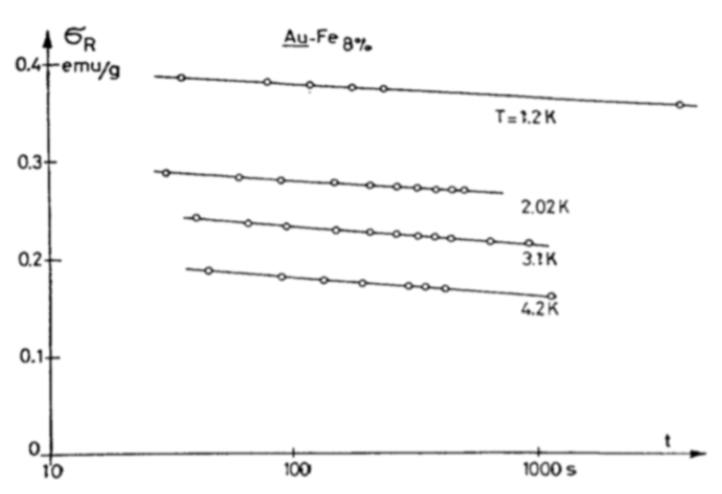
\includegraphics[width=0.6\textwidth]{img/remenant.png}
  \caption{ \label{fig:au-fe-remanent}Remanent magnetization of Au-Fe alloys plotted vs. time (logarithmic scale)for several temperatures, from \citet{Holtzberg1977}.}
\end{figure}
%Specific heat

\subsection{Specific Heat}

The specific heat of various spin glass materials has been measured and analyzed. 
In figure \ref{fig:cu-mn-cv}, we show the temperature dependence of magnetic 
specific heat of CuMn with 1.2\% Mn. The arrow on the x-axis indicates the spin glass
transition temperature $T_g$. The data shows a broad maximum above $T_g$, with no
anomaly at $T_g$. Below $T_g$, the specific heat exhibits $T$-linear behavior.

\begin{figure}
  \centering
  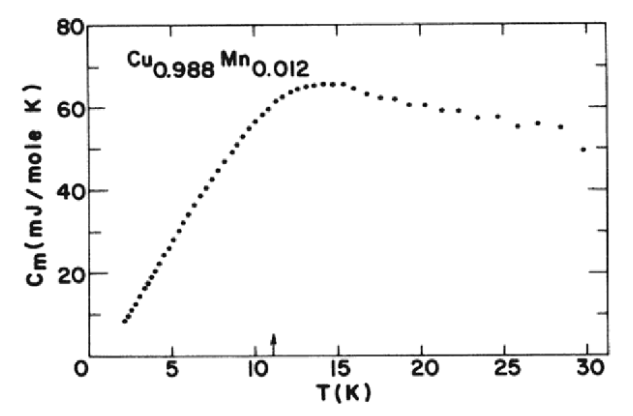
\includegraphics[width=0.6\textwidth]{img/cv.png}
\caption{\label{fig:cu-mn-cv}Magnetic part of specific heat of a Cu-Mn alloy plotted vs. temperature. Arrow shows where susceptibility has its cusp, from \citet{PhysRevB.13.4053}.}
\end{figure}

  

\iffalse
\begin{figure}[!h]
  \label{fig:experimentsSG}
  \centering
  \subfigure[Low frequency susceptibility of CuMn with 1\% Mn, from \citet{PhysRevB.23.1384}]
  {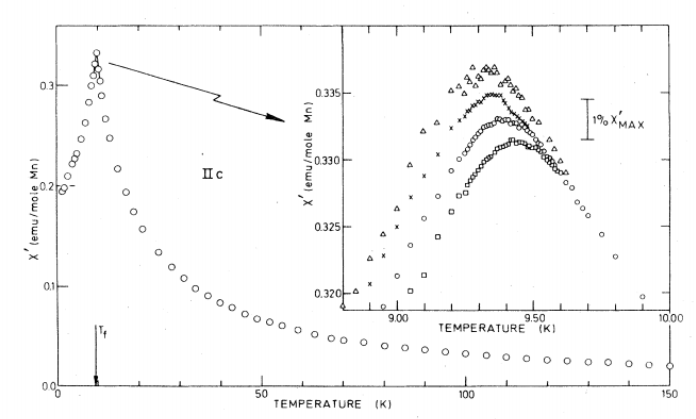
\includegraphics[width=0.6\textwidth]{img/cusp_low_freq.png}}\\  
\subfigure[Susceptibilities of CuMn vs temperature for 1.08\% and 2.02\% Mn, from 
\citet{PhysRevB.19.1633}]
{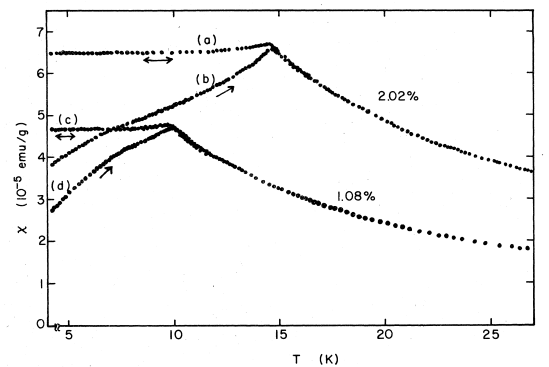
\includegraphics[width=0.6\textwidth]{img/fc_zfc.png}}
  \caption{Magnetic features of spin glass in a small field.}
\end{figure}
\fi


Other properties, such as DC susceptibility\citep{PhysRevB.19.1633,doi:10.1143/JPSJ.62.4488}, 
imaginary part of AC susceptibility\citep{PhysRevB.25.515,:/content/aip/journal/jap/53/3/10.1063/1.330780}, etc.,
were also extensively studied. 
These experimental facts suggest that spin glass system has no conventional 
long range magnetic ordering and exhibits very slow dynamics. For experimental 
systems, equilibrium can never be achieved. 


This cusp in the low frequency a.c. susceptibility set off the theoretical interest of spin glass physics. 
These behaviors are in sharp contrast of conventional magnetic system, say a ferromagnet. 
The susceptibility diverges at the critical point, the susceptibility
in this case is the linear response function to the field. This can be understood as the conjugate
variable of the magnetization, defined as $M=lim_{N \rightarrow \infty} <s_{i}> / N$, is the linear magnetic field. 
The spins point to a fixed preferential direction in the ordered phase. The cusp in the susceptibility has long been associated as the defining nature of a spin glass system. However, if the spin glass transition is a truly thermodynamic transition, we expect divergence in the response function corresponding to the order parameter. 

It was soon found by Edwards and Anderson that the order parameter should be characterizing an order in which each individual spin can point to a fixed direction, but the direction for each spin is random. The original form of the Edwards-Anderson 
order parameter can be defined as $Q=lim_{N \rightarrow \infty} <s_{i}>^{2} / N$. It is clear the absence 
of the divergence in the usual linear response is due to that the conjugate variables of an external field is not
divergence. If the magnetization is expanded in term of the magnetic field for two lowest orders, we can define
the non-linear susceptibility, $M=\chi h - \chi_{nl} h^{3}$, where $\chi_{nl}$ is the non-linear susceptibility. 
One can easily show that the non-linear susceptibility is proportional to the spin glass susceptibility as 
the fluctuations of the Edwards-Anderson order parameter $Q$. 

The direct evidence of a thermodynamic spin glass transition can be deduced from the study of the non-linear
susceptibility. The measurement is usually done by superconducting-quantum-interference-device (SQUID). The 
non-linear susceptibility can be extracted from the curve of the magnetization as a function of magnetic field.
This provides a direct access to the critical temperature and the exponent for the spin glass susceptibility. 

\section{Theoretical Understanding on Spin Glass}
A simple model that captures the consequences of disorder is an Ising model 
with quenched randomly disordered couplings, first proposed by Edwards and 
Anderson\cite{Edwards-Anderson1975}:
\begin{equation}
  \label{eq:Edwards-Anderson}
  H=-\sum_{\langle i,j \rangle}J_{ij}S_iS_j-h\sum_iS_i
\end{equation}
Here $S_i$ is the spin in a $d$-dimensional lattice that can take values $\pm 1$,
$\langle i,j \rangle$ indicates nearest neighbors with the coupling $J_{ij}$ between 
them, and $h$ is the external field.
 
Numerical evidence suggests that the criticality of the three-dimensional
spin glass systems are largely independent of the distribution of the randomness,
that is they are in the same universality class for different distributions. 
But, the two main paradigmatic cases for the $J_{ij}$ in Edwards-Anderson model are:
\begin{itemize}
\item Gaussian distribution of random coupling:
  \begin{equation}
    \label{eq:Jij_Gaussian}
    P(J_{ij})=\frac{1}{\sqrt{2\pi}}\exp^{-J_{ij}^2/2}
  \end{equation}
\item Bimodal ($\pm J$) distribution of random coupling:
  \begin{equation}
    \label{eq:Jij_bimodal}
    P(J_{ij})=\frac{1}{2}[\delta(J_{ij}-1)+\delta(J_{ij}+1)]
  \end{equation}
\end{itemize}

\subsection{Frustration}
\label{sec:frustration}
Frustration naturally presents in the Hamiltonian in Eq \ref{eq:Edwards-Anderson}, when no spin 
configurations can satisfy all couplings at the same time. 
Figure \ref{fig:frustration} demonstrate two situations where frustrations 
happens. In Fig \ref{fig:frustration_geo}, the two spins on the top and the left
are anti-parallelly aligned due to the antiferromagnetic coupling between them,
but there is not a preferred spin direction for the third spin that can satisfy
both the antiferromagnetic bonds. In Fig \ref{fig:frustration_quench}, the 
frustration comes from the random distribution of $J_{ij}$. 

\begin{figure}
  \centering
  \subfigure[Geometrical Frustration. Here all couplings are anti-ferromagnetic.]{
    \label{fig:frustration_geo}
    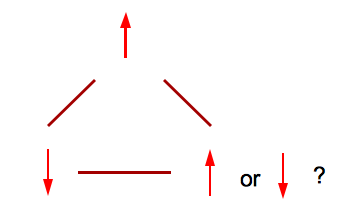
\includegraphics[width=0.4\textwidth]{img/ising-3-spin.png}
  }\hspace{0.5cm}
  \subfigure[Frustration due to randomness. Here $J=-1$ indicates an 
anti-ferromagnetic coupling, while $J=+1$ means ferromagnetic coupling.]{
    \label{fig:frustration_quench}
    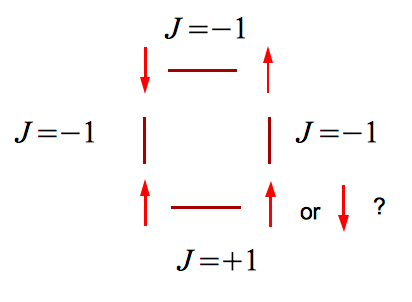
\includegraphics[width=0.4\textwidth]{img/ea-4-spin.png}
  }
  \caption{Frustration in Edwards-Anderson model.}
  \label{fig:frustration}
\end{figure}

The frustration is a key factor that leads to many features which make 
spin glass a complex system.
These features include: the existence of many metastable states; the rugged energy 
landscape; and dynamical behaviors such as slow relaxation, irreversibility, 
memory effects, hysteresis, etc. 


\subsection{Pictures on the Nature of the Spin Glass Phase}
\label{sec:meanfield-model}

An infinite-ranged version of spin glass models 
was proposed by Sherrington and Kirkpatrick (SK) \cite{Sherrington-Kirkpatrick-1975,Sherrington-Kirkpatrick1978}.
\begin{equation}
  \label{eq:SK}
  H=-\frac{1}{\sqrt{N}}\sum_{1\le i\le j\le N}J_{ij}S_iS_j
\end{equation}
Here $J_{ij}$ is chosen from a Gaussian distribution in equation 
\ref{eq:Jij_Gaussian}.
This model has an equilibrium phase transition at $T_c = 1$.
For the spin glass phase below $T_c$, Parisi\cite{Parisi1980,Parisi-1980b,Parisi-1980a} employed a novel ansatz and 
developed a  possible physical interpretation of the nature of spin glass, 
which is now known as the ``Replica Symmetry Breaking'' (RSB) picture. The main
idea behind the picture is that the spin glass phase consists of an infinite 
number of ``pure states'' that form a hierarchy rather than follow simple symmetry
transformation. 
The ultrametric topology of spin glass states can be represented with a 
genealogical tree. Each end point corresponds to a pure state, and branches 
represent clusters, as sketched in Fig. \ref{fig:TreeRSB}. 

%http://lptms.u-psud.fr/membres/Mezard/Pdf/84_MGSTV_PRL.pdf
%insert tree picture here.

\begin{figure}[!h]
  \label{fig:TreeRSB}
  \centering
  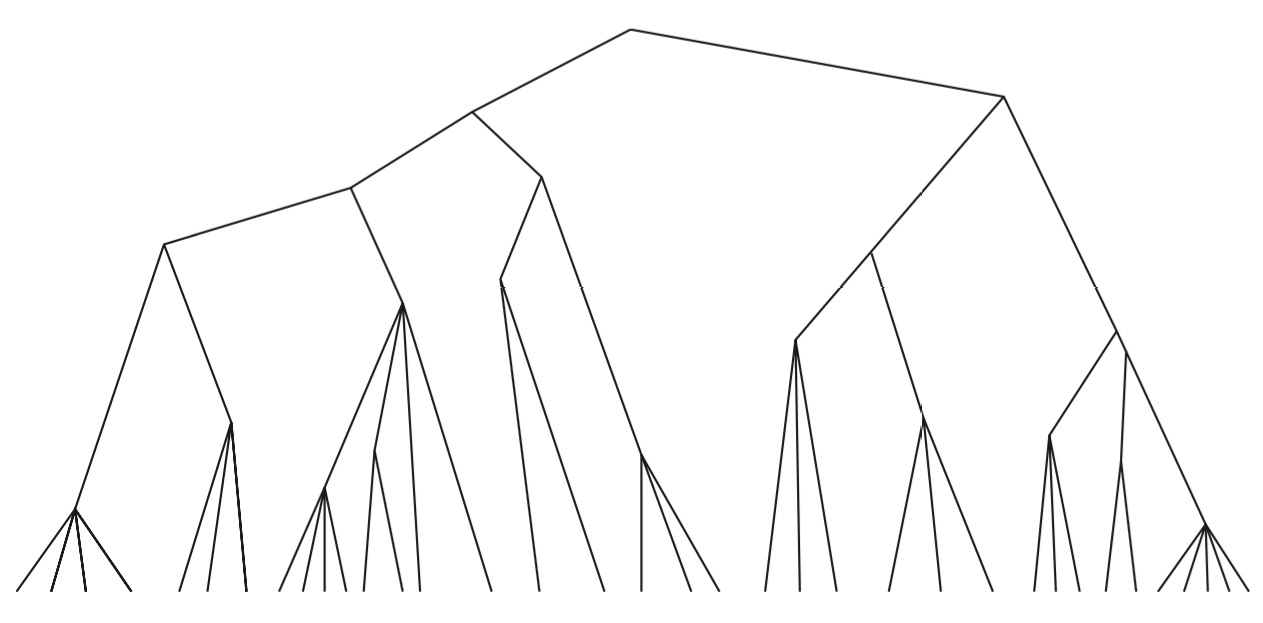
\includegraphics[width=0.6\textwidth]{img/TreeRSB.png}
  \caption{Hierarchical structure of the ensemble of spin-glass states, according
to the replica symmetry breaking picture. The end points represents states; branches (with all their descendents)
represent clusters.}
\end{figure}


Replica symmetry breaking is successful in the description of infinite range models, but whether it 
holds in finite dimensions remains the most prominent open question in the study of spin glass systems. 
A competing picture, known as droplet/scaling\cite{Fisher-Huse-1987,Fisher-Huse-1988}, 
is based on domain-wall 
renormalization group ideas. In this picture, there is only a single of
pure states that are spin-flip-symmetrical at low temperature in any finite 
dimension. The difference between the consequence from these two pictures 
will show up in the order parameters for spin glass as we will define in the following.

%\section{Quantities characterizing spin glass}

The quantity $q$ measures the overlap of the samples after a long time relaxation process. 
It was first studied by the seminal paper by Edwards and Anderson,
\begin{equation}
  \label{eq:q}
  q=\frac{1}{N}\sum_iS_i^\alpha S_i^\beta=\frac{1}{N}\lim_{T\to \infty}\sum_iS_i(t_0)S_i(t_0+T)
\end{equation}
where $\alpha$ and $\beta$ are two copies of lattice with the same disorder 
configuration, but simulated with different random seeds, so they are
statistically independent of each other. The Edwards-Anderson order paremeter, q, 
is the order parameter of measuring the breaking of ergodicity. 

The order parameter defined for the spin glass measuring the change of the systems
when the time goes to infinity. In the thermodynamic limit, if this
is zero, the system is ergodic, if this is finite, the system breaks
the ergodicity. Some parts of the phase space can never be sampled.

In contrast to conventional order parameters which measures the 
spatial pattern, such as magnetization. If the order parameter is non-zero, 
the system is said to undergo spontaneous symmetry breaking, in which the symmetry of 
the states is lower than that of the Hamiltonian. If one calculates
the Edwards-Anderson order parameter, said for the ferromagnet, it will
show a finite value. However, this is not a spin glass transition, a
spin glass transition does not come with a spontaneous symmetry breaking in space.

According to the Parisi solution, for fixed J and (large) N, the structure of 
the overlap is nontrivial, while in droplet picture, in the thermodynamic limit, 
the distribution is just a pair of delta functions at $\pm 1$. 
%insert figure for RSB/droplet overlap here

\begin{figure}
  \centering 
  \subfigure[Replica symmetry breaking picture]{
    \label{fig:overlap_rsb}
    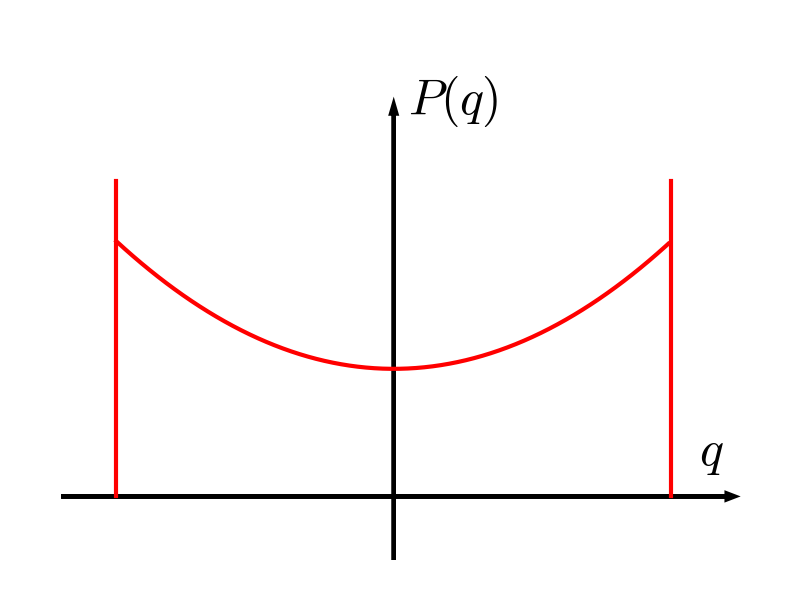
\includegraphics[width=0.4\textwidth]{img/sg/sg_rsb.png}
  }\hspace{0.5cm}
  \subfigure[Droplet picture]{
    \label{fig:overlap_droplet}
    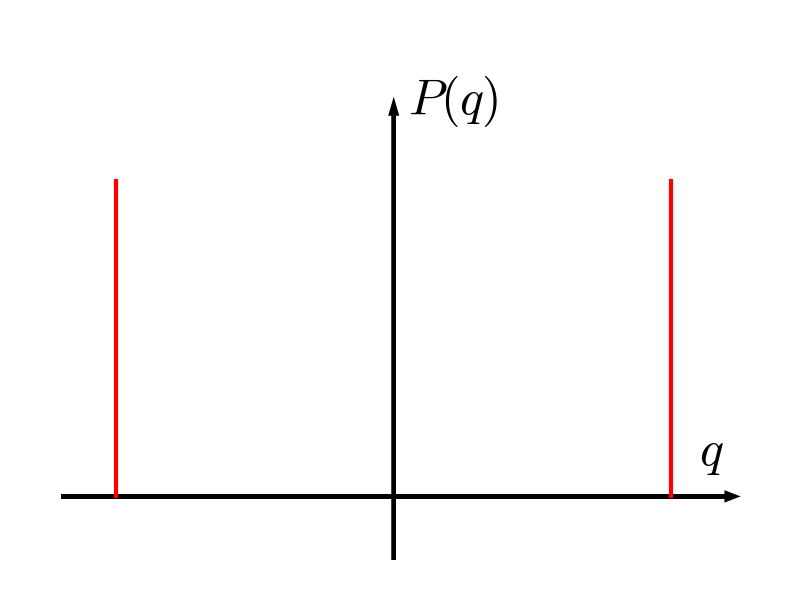
\includegraphics[width=0.4\textwidth]{img/sg/sg_droplet.png}
  }
  \caption{Sketch of the overlap distribution $P(q)$ for the replica symmetry 
breaking picture, and the droplet picture.}
  \label{fig:overlap}
\end{figure}

\section{Finite Size Scaling}
Most phase transitions can be described by an order parameter, which measures
the degree of order in a system. Usually, an order parameter is zero in one phase,
and non-zero in the other. At the critical point, the susceptibility of the order
parameter should diverge at the thermodynamic limit. An example of an order parameter is the 
magnetization in a ferromagnetic system. 
 
Second-order phase transitions, such as the magnetic transition in the Ising model, and 
spin glass transition in the Edwards-Anderson model, can be characterized by their 
power law behaviors for various quantities, such as heat capacity and susceptibility,  
close to the critical point. The systems can be categorized into different universality 
class according to the values of the exponents of these power law behaviors. For example, 
\begin{equation}
  \label{eq:20}
  \begin{array}{lrcl}
    \mathrm{Magnetization}& M& \sim& \left|T-T_c\right|^\beta\\
    \mathrm{Magnetic~susceptibility}& \chi_M& \sim& \left|T-T_c\right|^{-\gamma}\\
    \mathrm{Heat~capacity}& C_V& \sim& \left|T-T_c\right|^{-\alpha}\\
    \mathrm{Correlation~length}& \xi& \sim& \left|T-T_c\right|^{-\nu}
  \end{array}
\end{equation}

Close to the critical temperature, one can use the following ansatzes:
\begin{equation}
  \label{eq:17}
  M=L^{-\beta/\nu}g_M(tL^{1/\nu})
\end{equation}
\begin{equation}
  \label{eq:19}
  \chi=L^{\gamma/\nu}g_\chi(tL^{1/\nu})
\end{equation}
\begin{equation}
  \label{eq:18}
  C_V=L^{\alpha/\nu}g_C(tL^{1/\nu})
\end{equation}
where $t=(T-T_c)/T_c$.

A frequently used method to determine the critical point is to use
the intersection points of the Binder cumulants:
\begin{equation}
  \label{eq:14}
  U_L=\frac{1}{2}\left(3-\frac{\langle M^4\rangle_L}{\langle M^2\rangle^2_L}\right)
\end{equation}

For $T>T_c$, $\langle M^4\rangle_L = 3 \langle M^2\rangle_L^2$. 
For $T<T_c$, $\langle M^4\rangle_L = \langle M^2\rangle_L^2$.

As a result, the binder ratio
\begin{equation}
  \label{eq:16}
  U_L=\frac{1}{2}\left(3-\frac{\langle M^4\rangle_L}{\langle M^2\rangle^2_L}\right)
  =\left\{
    \begin{array}{ccc}
      0 & \mathrm{for} & T>T_c\\
      1 & \mathrm{for} & T<T_c
    \end{array}
  \right.
\end{equation}

At $T_c$, the Binder ratio does not depend on $L$ since
\begin{equation}
  \label{eq:15}
  \frac{\langle M^4\rangle_L}{\langle M^2\rangle^2_L}
  =\frac{L^{-4\beta/\nu}g_{M^4}(tL^{1/\nu})}{\left(L^{-2\beta/\nu}g_{M^2}(tL^{1/\nu})\right)^2}
  =g_c(tL^{1/\nu})
\end{equation}
therefore, $U_L$ tends towards an universal value independent of the system size.

So one can use various system sizes $L$, calculate $U_L$s as functions of $T$,
and find the point where the $U_L(T)$ curve cross to identify $T_c$. The catch
of the finite size scaling is that the power law scaling behavior is valid
only for the system is large, usually one would like to have the system
sizes to be larger than the correlation length. Even though, the finite size
scaling can in principle extract the exponent of the thermodynamic system,
it is still desirable to simulate large system sizes.
  
\section{Difficulties and Outstanding Problems}
The Edwards-Anderson model is a deceptively simple problem. Since it is a classical spin 
model, one may think that its numerical study can be simply carried out by Monte
Carlo methods on conventional hardware. One of the defining signatures of spin glass 
systems is their long relaxation time. 
For sufficiently low temperatures, the system becomes very sluggish and 
equilibration is prohibitively difficult even for modest systems sizes. 
Moreover, it has been shown that finding the ground state of the three-dimensional
Edwards-Anderson model is an NP-hard problem. \cite{Barahona-1982} 
Until recently, there has been no consensus on whether there is a finite spin 
glass critical temperature in the three-dimensional Edwards-Anderson model.

%It also requires a large number of disorder realizations to reach any 
%meaningful result.

Due to the difficulty in the simulation, there is still no general consensus on
which of the two competing pictures is correct. 
An import discriminator between the theories is the predicted behavior of 
the system when the temperature is decreased in the presence of an applied magnetic
field. 
In the mean-field approximation, the de Almeida-Thouless line separates the 
high-temperature paramagnetic phase from the spin glass phase (Fig.\ref{fig:at_rsb}). 
With the droplet/scaling theory, an applied magnetic field is predicted to remove
the phase transition completely (Fig.\ref{fig:at_droplet}).

\begin{figure}
  \centering
  \subfigure[Replica symmetry breaking picture]{
    \label{fig:at_rsb}
    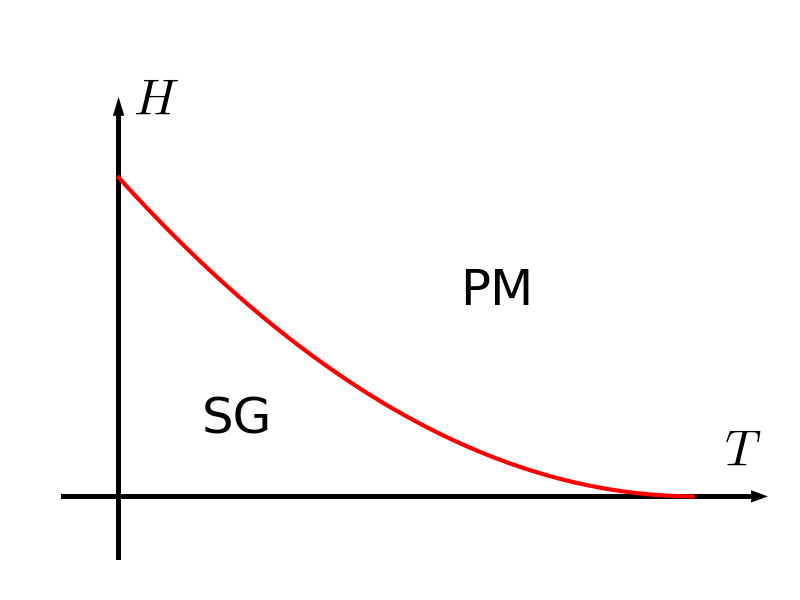
\includegraphics[width=0.4\textwidth]{img/sg/at_rsb.png}
  }\hspace{0.5cm}
  \subfigure[Droplet picture]{
    \label{fig:at_droplet}
    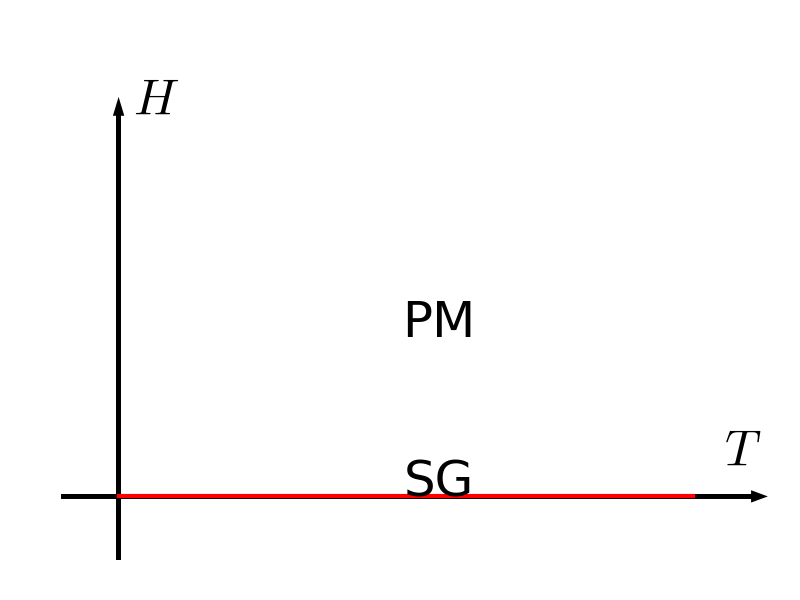
\includegraphics[width=0.4\textwidth]{img/sg/at_droplet.png}
  }
  \caption{Sketch of the de Almeida-Thouless line in the replica symmetry breaking 
picture, and the droplet picture.}
  \label{fig:at_line}
\end{figure}

Recent work supports that there is only a pair of two ground states in two dimensions.
In four dimensions, the JANUS show evidence for the presence of a spin glass
phase transition in a field. In three dimensions, numerical simulations give 
conflicting results.


\section{Algorithms for Spin Glass Simulation}
The breakthrough in the numerical study of spin glass systems came with the 
introduction of the parallel tempering method\cite{Swendsen-Wang-1986,Hukushima-Nemoto1996,Marinari-Parisi1992}. 
Parallel tempering (PT), also known
as replica exchange, is a simulation method aimed at improving the dynamic 
properties of Monte Carlo sampling. Instead of simulating one Markov chain at 
a time, one runs N copies of the system with random seeds at different 
temperatures and exchange configurations based on the detailed balance condition.
By making the configurations at high temperatures available to simulations at 
low temperatures, this method allows better sampling over the entire energy
landscape. We discuss this method further in \ref{sec:PT}.

Simulated annealing\citep{1983Sci...220..671K} is another commonly used algorithm for heuristic optimization,
due to its simplicity and effectiveness. In physics, one usually select the 
energy as the cost function, start the Monte Carlo simulation at a high temperature
and slowly tune down the temperature during the simulation, and in the end, the
configuration of the system would stay in a local minimum. With slow-enough annealing
and multiple repetitions, one would expect to find the global minimum.  

Population annealing\citep{2015PhRvE..92f3307W} combines simulated annealing and Boltzmann weighted 
differential reproduction within a population of replicas to sample equilibrium 
states. Similar to simulated annealing, population annealing involves lowering 
the temperature of the system at a sequence of temperatures. However, population annealing uses a 
population of replicas and this population is resampled at each time step.
By doing this, population annealing aims to ensure that the population always stay close to the 
Gibbs distribution. Population annealing is naturally a massively
parallel algorithm, as realistic spin glass simulation using population 
annealing require population sizes of the order $10^6$ or more.
%http://arxiv.org/pdf/1508.05647v2.pdf

Another possibility to overcome the diverging autocorrelation time problem is the 
multicanonical reweighting method\citep{1998PhyA..254..164J}. Instead of sampling the Boltzmann 
distribution $P=\exp(-\beta Ep)$, multicanonical ensemble uses the 
Metropolis–Hastings algorithm with a sampling distribution given by the inverse 
of the density of states of the system. The density of states has to be known 
a priori or be computed using techniques such as the Wang and Landau algorithm.



%%% Local Variables:
%%% mode: latex
%%% TeX-master: "../thesis"
%%% End:

\chapter{GPU Implementation}


This following chapter is a published work titled {\bf Parallel Tempering Simulation of the three-dimensional Edwards-Anderson Model  with  Compact Asynchronous Multispin Coding on GPU}.
In this paper, we discussed an efficient GPU implementation of Monte Carlo
Simulation of 3D Edwards-Anderson model, with parallel tempering and multispin 
coding technique. 

This paper is written in collaboration with Ye Fang, Ka-Ming Tam, Zhifeng Yun,
Juana Moreno, J. Ramanujam and Mark Jarrell. This work will also appear in 
Ye Fang's doctoral dissertation. 

Ka-Ming proposed this project in the first place. 
Ye Fang and I developed the implementation together. 
During the collaboration, I focused on the validity of the code, including the Monte Carlo
sampling procedures, the parallel tempering movements and the measurements,
and benchmarked the code against published results. Ye Fang dedicates his efforts
 on the efficiency of the code, including introducing and testing various 
multispin coding paradigms, optimizing the kernel organization, the memory access,
and core computation, and profiling the code to evaluate the performance. Ka-Ming
gave us a lot of advices through out the whole process. 

In the writing of this paper, Ye started the first draft. Ka-Ming contributed to
the physics 

\section{Introduction}

Stochastic or Monte Carlo (MC) simulation is one of the most important methods in 
the study of complex interacting systems. However, even with the huge success 
of Monte Carlo methods, many systems remain very difficult to simulate. 
The main obstacle very often is the long required simulation time, while 
the memory demands are quite modest. A prominent example is the Edwards-Anderson (EA) 
model, where the inherent randomness and frustration lead to very long relaxation 
times. Although the EA model has been intensively simulated over the 
past few decades, including implementations using gate-level reconfigurable processors 
\cite{Monaghan-1993} and some dedicated computers designed specifically for solving this model, 
\cite{Ogielski-Morgenstern-1985,Ogielski-1985,Cruz-2001,Condon-Ogielski-1985,Taiji-Ito-Suzuki-1988} 
many aspects are still far from completely understood. Some prominent 
topics, such as the nature of the spin glass phase below the upper critical 
dimension, remain highly debated issues.~\cite{Jorg-Katzgraber-Krzakala-2008,Moore-2005,Young-Katzgraber-2004,Temesvari-2008,Katzgraber-2008,Sasaki-etal-2008,Sasaki-etal-2007,Larson-etal-2013,Banos2012,Katzgraber-2012,Katzgraber-Larson-Young-2009,Leuzzi-2009}

The Graphics Processing Unit (GPU) provides an opportunity to 
significantly improve the computational performance of Monte Carlo simulations 
of classical systems. Massive parallelism and acceleration can be achieved by 
implementing these algorithms on GPUs. In the past few years some GPU accelerated 
simple spin models have been proposed, including the two-dimensional Ising model 
by \citet{CSTN-093} and \citet{2010CoPhC.181.1549B}, and the Ising model in the cubic 
and network lattices by \citet{Preis:2009:GAM:1537305.1537344}.
\citet{doi:10.1142/S0129183112400025,Weigel:2012:PPS:2151219.2151631}
studied the Ising and the Heisenberg models 
in both two- and three-dimensional lattices. These implementations focus 
predominately on unfrustrated systems with large lattice sizes. In this study, we mainly 
focus in the simulation of a random frustrated Ising system in equilibrium. 
Due to its slow relaxation rate, a large number of Monte Carlo 
steps are required, at the same time the system sizes that can be simulated are 
relatively small, in most cases limited to only a few thousands sites. Precisely 
because of these characteristics, Monte Carlo simulations of random frustrated 
systems are a good match for the GPU computing architecture.

Our implementation targets cluster computers with NVIDIA Fermi GPUs.
%and \q{may be} easily modified for other GPUs, e.g., Kepler GPU. 
Using C/CUDA we control and tune details of the program.
We expose the inherent parallelism of the algorithm
to the GPU accelerator, including parallel computation on multiple sites, multiple temperature 
replicas and multiple disorder realizations. The memory requirements are efficiently handled through
memory tiling. In addition, the computation is simplified and
vectorized using table look-ups and the Compact Asynchronous
Multispin Coding (CAMSC). We also substitute all floating point arithmetic
with integer or bit string computations while preserve the same
precision. Combining various tuning techniques, we achieve an average
spin flip time of 33.5 picoseconds. This is the fastest GPU
implementation for the random frustrated Ising system on a $16^3$
cubic lattice, and is comparable to that obtained with a field
programmable gate array (FPGA) hardware \cite{2012arXiv1204.4134J} for
small to intermediate system sizes. We note that a very recent preprint reported a faster speed in
a new FPGA system \cite{Janus2-2013}. 

The paper is organized as follows. In Section 2, we discuss the algorithm. In section 3, 
we present an outline of the code framework. The implementation 
and optimization methods are described in Section 4. Section 5 shows the experimental  
results. Conclusions and future directions are described in Section 6. 



\section{Theoretical Background}


\subsection{Spin Glass}

The discovery of a plethora of unusual magnetic behaviors in disordered materials 
initiated the field of glassy systems.\cite{Binder-Young1986} Spin glasses are 
beyond the conventional description of long range magnetic ordering, e.g., 
ferromagnetic ordering. Some of their features, including their frequency-dependent 
susceptibilities and the discrepancy between zero-field and field cooling measurements, 
suggest that spin glasses have very slow dynamics. Notwithstanding most experimental spin 
glass systems, which exhibit glassy behavior, randomness and frustration 
seem to share some common properties. In real materials, 
dilution introduces randomness and directional or distance-dependent couplings, 
such as dipolar interactions in insulating systems and the Ruderman-Kittel-Kasuya-Yoshida 
coupling in metallic systems, introduce frustration. 

The simplest model that captures the consequences of disorder is an Ising model 
with quenched randomly disordered couplings. This model was first proposed by Edwards 
and Anderson. \cite{Edwards-Anderson1975} The mean field solution of the EA 
model for infinite dimensions was first attempted by Sherrington and Kirkpatrick. 
\cite{Sherrington-Kirkpatrick1978} However, the replica symmetric mean field solution was found to be 
unstable below the Almeida-Thouless line, \cite{Almedia-Thouless1978,Bray-Moore-1978}
a line in the temperature-field plane below which replica symmetry is broken. The difficulty 
of obtaining a stable solution was solved by Parisi with his replica symmetry breaking 
ansatz. \cite{Parisi-1979,Mezard-etal-1984,Parisi-1980a,Parisi-1980b,Parisi-1980c,Parisi-dirac-medal-2002} 
Although the mean field solution has been proven to provide the exact free energy for the spin glass phase 
in infinite dimensions, \cite{Talagrand-2006,Guerra-2003} the spin glass 
physics in finite dimensions, which presumably is more relevant to experiments, is 
still not fully understood. Indeed, it had long been debated whether a spin glass 
phase at finite temperatures exists in three dimensions.

The EA model may be deceptively simple. Since it is a classical spin 
model, one may think that its numerical study can be simply carried out by Monte 
Carlo methods on conventional hardware. One of the defining signatures of 
spin glass systems is their long relaxation time. For sufficiently low temperatures, the 
system becomes very sluggish and equilibration is prohibitively difficult  
even for modest systems sizes.  Moreover, it has been shown
that finding the ground state of the three dimensional EA model is
an NP-hard problem. \cite{Barahona-1982} Until recently, there has been no %universal 
consensus on whether there is a finite spin glass critical temperature in the three 
dimensional EA model.

The breakthrough in the numerical study of spin glass systems came with the 
introduction of the parallel tempering method. It allowed the study of larger 
systems at lower temperatures than the simple single spin flip %Monte Carlo 
method. \cite{Swendsen-Wang-1986,Hukushima-Nemoto1996,Marinari-Parisi1992} Combined with 
improved schemes for finite size scaling, it is now widely believed that the thermodynamic 
finite-temperature spin glass phase does exist in the three dimensional EA 
model~\cite{Ballesteros2000}. As the upper critical dimension of the 
model is six \cite{Harris-Lubensky-Chen-1976,Tasaki-1989,Green-Moore-Bray-1983}, a
prominent remaining question is the nature of the 
spin glass phase below the upper critical dimension~\cite{Young-Katzgraber2004}. 
In particular, if the spin glass can still be described by the replica symmetry 
breaking scenario, there should be an Almeida-Thouless line below the upper 
critical dimension. A possible test of whether the Almeida-Thouless 
line exists is to determine whether a spin glass phase exists under an external 
magnetic field. Correlation length scaling analysis seems to suggest the 
absence of the spin glass phase in cubic lattices when a finite external field is applied.\cite{Young-Katzgraber-2004} 
On the other hand, a recent study in four-dimensional lattices suggests that by using a different quantity for the 
finite size scaling analysis, a spin glass phase can be revealed. \cite{Banos2012} 
Given the relevance of spin glasses and the on-going controversy on the nature 
of the spin glass phase below the upper critical dimension, it is desirable to 
implement an efficient parallel tempering Monte Carlo algorithm using 
graphics processing units to accelerate the simulations. In this work we show that 
using the multispin coding method, \cite{Zorn-Herrmann-Rebbi-1981} an efficient Monte Carlo algorithm can be implemented 
on the GPU. 


\subsection{Edwards-Anderson Model}

We consider the EA Model \cite{Edwards-Anderson1975} on a 
simple cubic lattice. Spins on each lattice site have two states 
$S_i=+1$ or $-1$. The couplings $J_{ij}$ are between nearest neighbors. In this 
study, we focus on a distribution of the couplings which is bimodal with a mean 
value of zero. That is, there are equal numbers of anti-ferromagnetic and ferromagnetic 
couplings. The effect of the distribution is certainly a non-trivial problem. 
We choose to focus on the bimodal distribution  because it is best suited for multispin coding. 
In addition, a constant external field, $h$, is included in our implementation. 
The Hamiltonian is given by 

\begin{equation}
H = - \sum_{i,j} S_i J_{ij} S_j + h \sum_{i} S_i.
\end{equation}


\subsection{Single Spin Flip Metropolis Algorithm}

We implement the Metropolis algorithm as our sampling method. The spins are 
visited and tested for flipping according to the probability $P = \mr{exp}(-\beta\Delta E)$,
where $\beta$ is the temperature and $\Delta E$ is the energy change associated 
with the proposed spin flip. As the algorithm satisfies detailed balance, the sampling 
will generate a distribution according to the partition function provided that the 
simulation is performed long enough.  This type of Monte Carlo simulation is
called a Markov process, because the evolution of the state only depends on the state 
at the current step, and not on its history. 
% Another popular Monte Carlo algorithm for the Ising spin system is the heat bath algorithm

\subsection{Parallel Tempering}

For the simulation of glasses, the local single spin 
update algorithm is very slow in thermalizing the system. This problem is particularly 
severe when the temperature is close to the critical temperature for the second order 
transition. For certain spin glass models where random dilution is sufficiently 
large, some form of cluster algorithm can improve the rate of thermalization. Unfortunately, 
there is no efficient cluster methods for general spin glass systems. The possible exceptions are 
some random diluted systems or systems in low dimension \cite{Houdayer-2001,Liang-1992,Jorg-2005}. Various other methods have been proposed 
in the past to improve the rate of thermalization including the umbrella sampling, 
the multi-canonical method, and rejection-free methods. It is now widely accepted that 
the parallel tempering method is one of the most efficient algorithms for improving 
the thermalization rate of general spin glass systems.

Parallel tempering uses several samples of the system within a range of 
temperatures (Figure \ref{fig-pt}). The low temperature sample is more difficult 
to thermalize due to the larger barriers between low energy 
configurations~\cite{Marinari-Parisi1992,Hukushima-Nemoto1996}.
However, as the probability to swap the configuration between the high and the low temperature samples 
increases, the chance of the system to escape from a local minima in the low temperature sample also 
increases. The efficiency of such a parallel 
tempering move can be measured by the time it takes for a sample to perform a 
round trip along the temperature axis, that is from the lowest to the highest 
temperature and back to the lowest temperature. This largely depends on 
the system being simulated. Fine tuning the range of temperatures and the 
spacing between them is crucial to optimize the performance. Some 
recent proposals have been tested on the non-disorder Ising model \cite{PhysRevLett.101.130603,1742-5468-2006-03-P03018,jcp/124/17/10.1063/1.2186639}.
Models with explicit disorder such as the EA lack an efficient 
general method. For a practical GPU implementation, one also 
needs to consider the effect of the number of replicas on the performance.


\begin{figure}[ht]
  \centering
%  \includegraphics[width=0.4\textwidth] {../img/model/barrier.pdf}
  \includegraphics[width=0.8\textwidth] {img/barrier.pdf}
  \caption{Schematic diagram of the free energy landscape.  At high temperatures 
(small $\beta$) the barriers between configurations are reduced allowing the 
system to search through configurations more efficiently.}
\label{fig-pt}
\end{figure}






\section{The Framework}

\label{section_framework}

The GPU implementation is discussed in this and the following sections. 
In our replica exchange spin glass simulation we exploit three levels of parallelism:
%We discuss three levels of parallelism that we exploit in the replica exchange spin glass simulation: 
\begin{enumerate}
\item Several tens of thousands, or more,  of independent disorder realizations are required to 
obtain good statistics. 
% break long sentences
\item For each disorder realization, usually a few tens of systems at different temperatures   
are needed to study the physics, such as the possibility of a critical point. We 
denote these systems as temperature replicas.   In the parallel 
tempering simulation, different temperature replicas  communicate with each other only during 
the parallel tempering swap; these swaps are performed after every few Metropolis single spin sweeps 
of the lattice. 
\item We are mainly interested in systems on bipartite lattices. These are lattices that can 
be divided in two sub-lattices (A and B) with same sub-lattice spins 
do not directly coupling with each other. As a result, the update of the A sublattice 
is independent of the B sublattice. 
\end{enumerate}
These three levels of inherent parallelism allows an efficient GPU
implementation. In this section we focus on the main
structure of the code, which consists of three parts: (i) distributing
the spin updates into different GPU threads; (ii) distributing 
different disorder realizations into different GPU
blocks; and (iii) integrating and vectorizing the bit computations
of many temperature replicas

\subsection{Map Lattice Sites to GPU Threads}

\label{section_framework_threads}

The spin lattice is represented by a three dimensional primitive cubic system. To update the sites in 
the lattice, we follow the common practice of employing a checkerboard decomposition that 
splits the sites into two sub-lattices shown in blue and red in Figure \ref{fig_checkerboard} . 
Since a blue site is surrounded by red sites and never directly interacts with other 
blue sites and vice-versa, it is permissible to update each sub-lattice in parallel.  
We construct two consecutive stages concentrating 
independently on each of the sub-lattices for parallel computation. The combination of 
the two stages delivers a lattice sweep of Monte Carlo updates. The lattice is assigned 
to a GPU thread block, and sites are split across the threads. Details about the 
lattice site to thread mapping will be discussed in Section \ref{section_memory} 
where we discuss memory optimizations. The total available thread-level parallelism 
is half of the total lattice sites, and specifically, falls into the range between 
$8^3 / 2 = 256$ to $16^3 / 2 = 2048$ since our simulation targets lattices 
between $8^3$ to $16^3$ sites. 


\begin{figure}[ht]
  \centering
  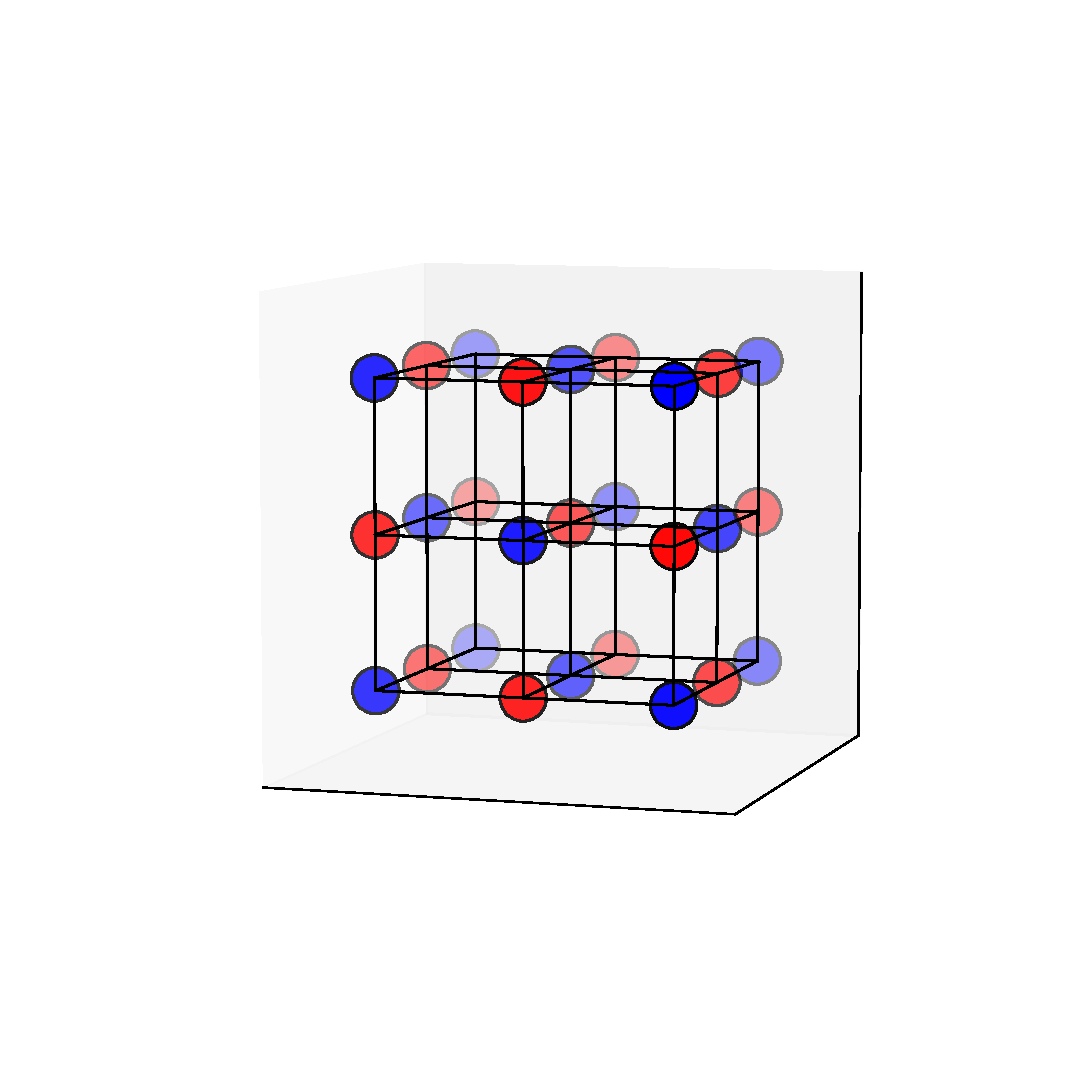
\includegraphics[width=0.6\textwidth] {img/checkerboard.pdf} 
  \caption{A demonstration of the 3D checkerboard decomposition. 
The blue and red sites are on different sub-lattices. 
Since the sites in a sub-lattice never directly interact with each other, 
it is permissible to update different sites in parallel. 
}

\label{fig_checkerboard}
  \end{figure}


\subsection{Map Temperatures Replicas to Bits} 

The parallel tempering technique facilitates the systems to achieve 
equilibrium. We choose the temperature as the tempering parameter and generate systems 
with the same couplings but different temperatures, called temperature replicas. The 
temperature replicas are uncorrelated during the spin-flip process and can therefore
be updated in parallel. However, they communicate and 
swap temperatures (Figure \ref{fig_bits}) after a few Monte Carlo sweeps. To better 
utilize the parallelism of multiple temperature replicas and minimize the communication 
overhead we have developed the Compact Asynchronous Multispin Coding (CAMSC), where 
spins from different temperature replicas at the same position are encoded into 
an integer. This leads to sub-word vectorization and a significant reduction of 
memory transactions. Details of our multispin coding procedure can be found in 
Section \ref{section_msc}. The number of temperature replicas depends on the 
system size and the temperature range. In our simulation we used 24 replicas 
for smaller systems, and 56 temperatures for bigger systems (for example, 
$10^3$ and $12^3$).  


\begin{figure}[ht]
  \centering
%  \includegraphics[width=0.35\textwidth] {../img/skeleton4_.pdf}
  \includegraphics[width=0.5\textwidth] {img/skeleton4_.pdf}
  \caption{Many temperature replicas can be simulated simultaneously, each 
using an independent Monte Carlo process. These replicas may be exchanged
after a configurable steps of updates. 
A single GPU thread block is responsible for updating all the Monte Carlo processes
and manipulating the parallel tempering exchange.
}
 \label{fig_bits}
  \end{figure}


\subsection{Map Realizations to GPU Blocks}


Spin glass simulations usually require a larger number of disorder realizations ($10^4$ or more) for reliable 
disorder averaging.  A realization including all temperature replicas has been designated to 
a thread block.  We launch numerous thread blocks across multiple GPUs of multiple hosts 
until we get the sufficient number of realizations for disorder averaging (Figure \ref{fig_tasks}). To distribute 
these jobs across multiple nodes, we employ a Pthreads/MPI wrapper for the job distribution. 

\begin{figure*}[ht]
  \centering
%  \includegraphics[width=0.95\textwidth] {../img/skeleton1_.pdf}
  \includegraphics[width=0.95\textwidth] {img/skeleton1_.pdf}
  \caption{The outline of the simulation application. Disorder realizations are completely 
independent and can run simultaneously. Each realization contains a unique 
Monte Carlo parallel tempering process as depicted in Fig.~\ref{fig_bits}, and is 
assigned to a GPU thread block. This task level parallelism yields sufficient number of  
thread blocks and can fully occupy a parallel computer system.
}
  \label{fig_tasks}
\end{figure*}
 



\subsection{Discussion}

Some parallel processes are sequentialized for better memory
locality. For example, although the temperature replicas could be
fully parallelized as individual tasks or a lattice may be partitioned
across multiple thread blocks, we avoid these forms of parallelism.
The remaining parallelism is rich enough (with $10^4$ or more 
thread blocks) to fully occupy the cluster. % parallel computer

% add some words to explain that single GPU performance metrics is a fair measurement

To evaluate %"qualify"
the performance, we employ a performance metric of
average time (in picoseconds) per proposed spin flip for a single GPU card:
\begin{equation}
  \label{eq:tsf}
  t=T_\mathrm{total} / N_\mathrm{MCS} / \left( N_\mathrm{spins} \times N_T \times N_\mathrm{samples} \right),
\end{equation}
where $T_\mathrm{total}$ is the total wall time of a simulation;
$N_\mathrm{MCS}$ is the number of Monte Carlo sweeps;
$N_\mathrm{spins}$ is the number of spins within a lattice;
$N_T$ is the number of temperature replicas;
$N_\mathrm{samples}$ is the total number of disorder realizations on one GPU card.
We develop and benchmark the code on a NVIDIA GeForce GTX 580 GPU. Detailed
platform configurations can be found in Section \ref{section_exp}.




\section{Implementation}




\label{section_implementation}

We discuss implementation details in this section, including the
construction of the GPU kernel, memory optimization, and various
techniques used to simplify the computation.


\subsection{Kernel Organization Optimization}

\label{section_korg}

Our simulation starts with the Pthreads/MPI job dispatcher that 
forks many CPU processes across the cluster computer system. Each CPU
process is responsible for initiating a
lattice realization, which is offloaded to its attached GPU 
for simulation until the spin variables or thermal averaged results are 
retrieved from the GPU back to the CPU for analysis. 
%No CPU-GPU communication is needed during this simulation.

The GPU workload has three major components (Figure \ref{fig_korg1}):
\begin{enumerate}
\item {\bf Metropolis moves}: The Metropolis steps for the single spin
  update for each temperature replica. This is done by calculating
  the local energy change and then comparing the acceptance ratio to a
  uniformly distributed random number.
\item {\bf Parallel tempering moves}: Parallel tempering swaps are
  performed after a few complete Monte Carlo sweeps of the
  lattice. This step requires the calculation of total energy for all
  temperature replicas; we use this to evaluate the acceptance ratio
  of parallel tempering swaps.
\item {\bf Measurements}: The spin configurations are dumped to the
  GPU global memory periodically to provide data for the
  measurements. In practice, we perform one measurement for every few
  thousands Metropolis sweeps.
\end{enumerate}


\begin{figure}[ht]
  \centering
%  \includegraphics[width=0.35\textwidth] {../img/skeleton2_.pdf}
  \includegraphics[width=0.6\textwidth] {img/skeleton2_.pdf}
  \caption{Three major components of the GPU program. 
One kernel calls Monte Carlo and parallel tempering, implemented as 
two device functions. Measurement is implemented as a separate GPU kernel.} 
  \label{fig_korg1}
  \end{figure}

The measurement code has little overlap with the Monte Carlo and
parallel tempering codes, and it is called much less frequently. We
implement this part of the code as an separate GPU kernel.

Both Monte Carlo and parallel tempering functions compute spin local
energies. Parallel tempering requires additional steps to sum the
local energies. Since an efficient implementation of sum (a form
of reduction)
consumes a considerable amount of shared memory, it may be efficient
to separate the parallel tempering as a dedicated GPU function
apart from the Monte Carlo. We denote this scheme {\bf MC-PT
  separated}. Alternatively, the {\bf MC-PT integrated} scheme
combines both the Monte Carlo and parallel tempering in a single GPU
kernel. Benchmarks (Figure \ref{fig_korg}) show that the 
{\bf MC-PT separated} scheme always performs better regardless of the frequency of
parallel tempering. However, we find that roughly 10 full Monte Carlo
sweeps of the lattice between parallel tempering attempts is a
speed/effectiveness sweet point.

\begin{figure}[ht]
%  \includegraphics[width=0.5\textwidth] {../img/perf/korg.pdf}
  \centering
  \includegraphics[width=0.8\textwidth] {img/korg.pdf}
  \caption{A comparison of the performance of the {\bf MC-PT integrated} and the {\bf MC-PT separated} schemes
with different numbers of Monte Carlo sweeps between an attempted parallel tempering swap.
The test is conducted with a $16^3$ cubic lattice, shared memory probability table of integers, CURAND, 
and CAMSC. }
  \label{fig_korg}
  \end{figure}

%We measure and collect data every 1000 Monte Carlo sweeps. The GPU kernel performs 1000 Monte 
%Carlo sweeps and attempts 100 parallel tempering swaps between measurements. The lifespan of a GPU 
%kernel call is around 200 milliseconds, which is large enough comparing with the launch overhead. 


\subsection{Memory Optimization}

\label{section_memory}


Each spin interacts with its six nearest neighbors (Figure
\ref{fig_stencil}) as a seven-point 3D stencil
\cite{Nguyen:2010:BOS:1884643.1884658, Datta:2008:SCO:1413370.1413375} with periodic boundary
conditions.  Unlike some stencil problems, e.g., the Jacobi finite
difference solver for partial differential equations, in which the
data for the new time step is completely based on the previous time
step, the checkerboard decomposition allows the spin glass simulation
to proceed with two consecutive update phases. Only half of the spins are
updated in each of the phases. This unconventional stencil, associated
with the checkerboard decomposition, leads to a stride-2 memory
reference pattern and presents a more challenging memory optimization
problem compared to the stride-1 pattern of typical stencils problems.



\begin{figure}[ht]
  \centering
%  \includegraphics[width=0.25\textwidth] {../img/model/near.pdf}
  \includegraphics[width=0.4\textwidth] {img/near.pdf}
  \caption{The memory access pattern for a single spin update where in
    addition to the state of the local spin, we also need the states
    of its 6 neighbors. Periodic boundary conditions are used.}
\label{fig_stencil}
\end{figure}



\subsubsection{Allocation}

%We use a form of the multispin coding method to represent many replicas of spins lattices in an integer array the m Compact Asynchronous Multispin coding (CAMSC) (section \ref{section_msc})) 

We propose three different schemes to address this problem.
\begin{enumerate}
\item The {\bf Unified} allocation (Figure \ref {fig_alloc12}(a))
  stores the checkerboard lattice in its native way as a single piece.
\item The {\bf Separated} allocation (Figure \ref{fig_alloc12}(b))
  breaks the sub-lattices into two chunks stored separately.
\item The {\bf Shuffled} allocation \cite{2008CoPhC.178..208B} (Figure
  \ref{fig_alloc3}) mixes and integrates two temperature replicas,
  so that the memory access pattern is now identical to the
  conventional stencil.  This is done by mixing the two temperature
  lattices in such a way that all the A sublattice spins from
  temperature 1 and the B sublattice spins from temperature 2 are
  packed together in the memory associated with one lattice. When the
  spins are being updated on this lattice, they are all independent
  of each other. They can be considered sequentially and
  continuously written into memory. Since there is no gap between each
  memory write, this should theoretically enhance the memory access
  speed.
\end{enumerate}

The performance comparison on Table \ref{table_allocation} suggests that the
separated allocation is inferior due to its significantly lower memory
performance. This is because of the more complicated control flows in
the code. 
%Between the other two memory allocation schemes, although
%shuffled allocation offers a higher memory bandwidth than unified
%allocation, fewer spins can be served per memory transaction (see
%multispin coding of Section \ref{section_msc}). 
Overall, the unified allocation provides the best memory performance
in terms of time spent for each spin and is used in our
implementation.

\begin{figure}[!h]
  \centering
%  \subfigure[Unified]{\includegraphics[width=0.15\textwidth]{../img/memory/check_2_shared.pdf}}\hspace{1.4cm}
\subfigure[Unified]{\includegraphics[width=0.3\textwidth]{img/check_2_shared.pdf}}\hspace{1.4cm}
%  \subfigure[Separated]{\includegraphics[width=0.173\textwidth]{../img/memory/check_2_separated.pdf}}
\subfigure[Separated]{\includegraphics[width=0.346\textwidth]{img/check_2_separated.pdf}}
  \caption{Unified and separated memory allocation schemes.  The unified scheme stores the entire checkerboard
  lattice together. The separated scheme breaks the memory associated with each sublattice into
  separate continuous blocks of memory.}
\label{fig_alloc12}
\end{figure}



\begin{figure}[!h]
  \centering
%  \includegraphics[width=0.4\textwidth] {../img/memory/check_2_shuffled_.pdf}
  \includegraphics[width=0.7\textwidth] {img/check_2_shuffled_.pdf}
\iffalse
  \caption{The shuffled allocation mixes and integrates the lattice of spins from 
two temperature replicas so that the memory access pattern is now identical to the 
conventional stencil.  The two original temperate replicas are show on the top and
bottom left.  To form the to middle lattice we take the spins from the A sublattice
on the top (large orange circles) and the B sublattice on the bottom (large blue
circles).  The bottom middle lattice is formed similarly from the small circles).
The memory pattern on the transformed lattices (right) is close to that of a 
conventional stencil. We integrated two transformed lattices in different bit 
positions of the compact multiSpin coding scheme (Section \ref{section_msc}), to 
avoid doubling the amount of memory consumed. }
\fi

  \caption{The shuffled allocation mixes and integrates two lattices,
shown on the top of the figure. The first transformation is taking
the A sublattice on the left (blue dots) and the B sublattice
on the right (blue circles) to construct an intermediate lattice
(middle left figure of blue color).
Another intermediate lattice of red color is constructed similarly.
We then integrate these two intermediate lattices together, which
occupy different bit positions under the compact multispin coding scheme (Section \ref{section_msc}).
By using one integer lattice instead of two, we avoid doubling the memory consumption.
Also, the memory access pattern is identical to that of the 7-point 3D Jacobi stencil.
}



\label{fig_alloc3}
\end{figure}


\begin{table}[h]
\begin{small}
  \begin{tabular*}{\hsize}{@{\extracolsep{\fill}}lccc@{}}
    \hline
                                 & Unified       & Separated     & Shuffled\\
    \hline
    Bandwidth(GB/s)              & 645.1         & 279.0         & 832.6\\
    Time per transaction (ps)    & 49.608        & 107.756       & 38.432\\
    Spins per transaction        & 24            & 24            & 16\\
    Time per spin (ps)           & 2.067         & 4.345         & 2.402\\
    \hline
  \end{tabular*}
\end{small}
  \caption{Performance comparison of the unified/separated/shuffled storage allocation schemes for
  a $16^3$ lattice. The definition of  a transaction is a sequence of  7 loads and a store that serve the spin update.}
\label{table_allocation}
  \end{table}



\subsubsection{Tiling for the Multispin Coding Lattice}
The basic idea of multispin coding (MSC) is to present many binaries or short vectors in a longer 
packed word. For example, Ising spins may be stored with a single bit per spin, with 0 being spin 
down and 1 being up.  In our particular implementation, we also encode the 4 bit string of one site's 
spin-flip probability table's row index (section \ref{section_prob}) into an integer word. 
MSC \cite{PhysRevLett.42.1390,Zorn-Hermann-Rebbi-1981} yields a more efficient way of calculating local energies 
($E$) and reduces the memory required for the spin configurations.  This packing prevents the Arithmetic 
Logic Unit, which performs integer arithmetic and logical operations, and the memory bandwidth from 
being under utilized. Also, a memory transaction (7 loads and 1 store) can serve the calculation of 
multiple spins, which helps improve the relative memory performance.

The usual practice for a single lattice MSC is integrating a line of
spins into an integer. We denote this conventional method as
Synchronous Multispin Coding ({\bf SMSC}). For the simulation of spin
glass models, the temperature replicas provide an alternative approach
with a different memory layout.  One can pack the spins at a
specific site but at different temperature replicas into an integer;
we call this the Asynchronous Multispin Coding ({\bf AMSC}). The main
idea of these two multispin coding schemes are:
\begin{itemize}
\item {SMSC}: A packed word stores the spins from a single replica, but
  different sites.
\item {AMSC}: A packed word stores the spins belonging to different
  temperature replicas of the same site.
\end{itemize}
We find the ASMC scheme to be more efficient. Its storage consumption
is small enough to fit in the GPU shared memory. Furthermore, AMSC's
index system is more straightforward, thereby simplifying
optimization.  The performance of these different MSC schemes is
described below.  Here, we briefly discuss how the words
associated with either scheme are organized into memory.

Three levels (Figure \ref{fig_tile}) of the memory hierarchy are employed
that reflect the GPU memory architecture of global memory, shared
memory and registers:
\begin{itemize}
\item {\bf Level 1:} The main data resides in the GPU global
  memory. Due to the limitation that a 32 bit integer represents at
  most 32 spins, we may need multiple integer cubes (with an integer
  cube including one integer per site on the cubic lattice) if there
  are more than 32 temperature replicas.

\item {\bf Level 2:} The shared memory scratchpad holds the working
  set of an entire integer cube (no larger than $4 \times 16^3 =
  16KB$).  The data transfer between global and shared memory is quite
  modest because we do not need to switch to another integer cube
  until the Monte Carlo and parallel tempering swaps within the
  temperature replicas contained within the current cube are
  exhausted.

\item {\bf Level 3:} The GPU threads scan the shared memory scratchpad
  for two consecutive sublattices and load the data into
  registers. The threads are organized as multiple layers of 2D
  plates.  We observe the optimal thread configurations are two or
  four layers ($16^2/2 \times 2 = 256$ or $16^2/2 \times 4 = 512$).
\end{itemize}

\begin{figure}[!h]
  \centering
%  \subfigure[Global Memory]{\includegraphics[width=0.19\textwidth]{../img/memory/tiling4_1.pdf}}\hspace{0.2cm}
%  \subfigure[Shared Memory]{\includegraphics[width=0.12\textwidth]{../img/memory/tiling4_2.pdf}}\hspace{0.2cm}
%  \subfigure[Registers]{\includegraphics[width=0.1\textwidth]{../img/memory/tiling4_3.pdf}}
  \subfigure[Global Memory]{\includegraphics[width=0.38\textwidth]{img/tiling4_1.pdf}}\hspace{0.2cm}
  \subfigure[Shared Memory]{\includegraphics[width=0.24\textwidth]{img/tiling4_2.pdf}}\hspace{0.2cm}
  \subfigure[Registers]{\includegraphics[width=0.2\textwidth]{img/tiling4_3.pdf}}

  \caption{Memory tiling.  The global memory may hold several integer cubes (including one integer
per lattice site) if there are more than 32 temperature replicas.  The shared memory scratchpad holds 
the working set of an entire integer cube (no larger than $4 \times 16^3 = 16KB$).  The registers hold the
data needed for local spin updates.}
  \label{fig_tile}
\end{figure}



\subsection{Optimizing the Computation}

\label{section_compute}
%We look into the computation behaviors of GPU threads, try to transfer the data representations, simplify computations and employ sub-word vectorizations.

We may take advantage of the MSC mapping of the spins onto bits to
dramatically reduce the number of floating point operations needed by
the Monte Carlo parallel tempering calculations.  
For example, we may use a bitwise XOR ($\oplus$) as
opposed to multiplication to calculate the energy. In the equations
below, we denote the variables in the original notation with a
superscript $^o$, and variables without superscripts are used in the
transformed notation. The variables $S$,
$J$, $e$ and $E$ stand for
spin, spin coupling, bound energy and local energy respectively.


%The variables is mapped from their original notations to a computational optimizaed notation. This dramatically 
%simplifies the operations, for example, used bitwise XOR ($\oplus$)as apposed to the multiplication. We denote 
%the variables in the original notation with a superscript ``$^o$'', and without supscripts for transformed notation. 
%$\boldsymbol{S}$, $\boldsymbol{J}$, $\boldsymbol{e}$ and $\boldsymbol{E}$ stand for spin, spin coupling, bound 
%energy and local energy respectively.

\[
S^o \in \{-1, 1\}, J^o \in \{-1, 1\}
\]
\[
E^o_{i} = \sum_{j} S^o_i \times J^o_{ij} \times S^o_j, E^o_{i} \in \{-6, -4, -2, 0, 2, 4, 6\}.
\]
\[
S \in \{0, 1\}, J \in \{0, 1\}
\]
\[
E_{i} = \sum_{j} S_i \oplus J_{ij} \oplus S_j, E_{i} \in \{0, 1, 2, 3, 4, 5, 6\}.
\]
Note that local energy $E^o_{i} $, the energy of a spin $i$ in the field of its nearest neighbors, can only take 
one of seven values as indicated.  
%(\oplus \textrm{ represents bit wise XOR})

The computation is composed of four steps:
\begin{enumerate}
\item Energy:
Compute the bound energy ($e$) and the spin's local energy ($E$).
\begin{align}
\label{eq:e}
\begin{split}
e_{ij} = S_i \oplus J_{ij} \oplus S_j\\
E_{i} = \sum_{j} e_{ij}
\end{split}
\end{align}

\item Probability:
Compute the flip probability ($P$) for the Metropolis Monte Carlo,
where the temperature ($T$) is an input parameters.
% alternative:
% where using Temperature ($T$) as an input parameters.
\begin{align}
\begin{split}
\label{eq:p}
E^o = 2 \times E - 6 \\
S^o = 2 \times S - 1 \\
P = \mr{exp} (2 \times (\frac{1}{T} \times E^o + h \times S^o))
\end{split}
\end{align}

\item Rand:
Generate a random number ($R$).

\item Compare:
Compare and update spins.
\begin{equation}
\label{eq:r}
S = (P < R) \oplus S.
\end{equation}
\end{enumerate}





\subsubsection{Probability Look-up Table}

\label{section_prob}

Eq. \ref{eq:p} expresses the straightforward yet expensive method to generate the spin flip 
probabilities. However, since the number of input/output values is finite (i.e., combinations of 7 
possible local energies $E$, 2 spins $S$, and no more than 32 temperatures $T$), a better solution 
is to deploy a pre-calculated look-up table. The table is a two-dimensional matrix (Figure \ref{fig_table}), 
with $T$ as the row index and $(E \times 2 + S)$ as the column index.  The column index, as the 
combination of $E$ and $S$, requires 4 bits for the address space. The maximum storage consumption 
of the table is 16 KB, assume that we have 32 rows times 14 columns times 4 bytes per entry (again, 
assume 32 temperature replicas).  When a parallel tempering swap between two replicas at temperatures 
$T_{i}$ and $T_{j}$ is accepted, the two corresponding rows in the table are swapped. 




\begin{figure}[!h]
  \centering
%  \includegraphics[width=0.45\textwidth]{../img/table1.pdf}
  \includegraphics[width=0.6\textwidth]{img/table1.pdf}
  \caption{The organization of the probability look-up table.}
\label{fig_table}
\end{figure}

We evaluate four different ways to calculate the probability in Eq.~\ref{eq:p} (Figure \ref{fig_perf_prob}): 
(a) using the floating point exponential function from the math library, 
(b) using a less accurate GPU specialized exponential intrinsic function, 
(c) using the texture memory to store a table, and 
(d) a shared memory table. 
The result shows that an optimal table look-up saves close to half of the total computation time
%up to 73\% %(94.929 - 54.661) / 54.661 
compared to direct computation of the probabilities. In addition, 
the shared memory table outperforms the texture memory table. This is
because GPU threads are simultaneously computing on the same
temperature replica, and are therefore accessing the same row of the
table. This avoids bank conflicts, so that the high bandwidth and low
latency performance potential of the shared memory is fully exploited. 
% is utilized -> delivers its maximum performance potentia


\begin{figure}[!h]
  \centering
%  \includegraphics[width=0.45\textwidth]{../img/perf/prob1.pdf}
  \includegraphics[width=0.8\textwidth]{img/prob1.pdf}
  \caption{A comparison of the overall time consumed per spin flip 
using four different methods to compute the exponential probability in 
Eq.~\ref{eq:p} as described in the main text. 
The experiment is done for a $16^3$ lattice, fp32 CURAND and AMSC1. 
  No parallel-tempering is performed.}
  \label{fig_perf_prob}
\end{figure}
% regenerate the performance chart, remove integer table.


\subsubsection{Random Number Generator}

\label{section_rng}

The simulation requires uniformly distributed random numbers between
zero and one. However, due to the fact that pseudo random number
generators (RNGs) manipulate integer values internally, directly using integer
return values from the RNG provides higher performance and preserves identical
precision.  As a consequence, we convert the pre-generated
probabilities from single precision floating point numbers to 32 bit
unsigned integers.

We evaluated three random number generators: (i) NVIDIA CURAND library
of XORWOW algorithm \cite{curand}, (ii) rand123
\cite{Salmon:2011:PRN:2063384.2063405} philox4x32\_7 (version 1.06),
and (iii) our implementation of a multi-threaded 32 bit linear
congruential generator (LCG).  We decide to adopt CURAND due to its
higher performance (Figure \ref{fig_rng}) and quality
\cite{2012arXiv1204.6193M}.

%For Ising model without parallel-tempering, it is legal to update a spin among all temperature replicas using the same random number. That is, we just need one random number for all AMSC/CAMSC bits. This approach has impressive benefits on average update time per spin. However it does not shorten the wall-clock time needed for a simulation, \q{as it does not improve the time needed to follow the history of one system. Also, it provides fewer advantages as the system size increases, since single-system simulation time increases, while the required number of samples decreases due to the self-averaging property.}

\begin{figure}[!ht]
  \centering
%  \includegraphics[width=0.45\textwidth]{../img/perf/rng.pdf}
  \includegraphics[width=0.8\textwidth]{img/rng.pdf}
  \caption{A comparison of the overall time required per spin flip using different random number generators. 
  The experiment used a $16^3$ lattice, a shared memory probability table and CAMSC. No 
  parallel-tempering is performed. The loop that consumes random numbers has been unrolled four 
  times to match the four return values of rand123 philox4x32\_7.} 
  \label{fig_rng}
\end{figure}







\subsubsection{Multispin Coding}

\label{section_msc}

\begin{figure*}[ht]
  \centering
  %\includegraphics[width=\textwidth]{../img/msc/new_amsc1344.pdf}
%  \subfigure[AMSC1]{\includegraphics[width=0.267\textwidth]{../img/msc/new_amsc1.pdf}}\hspace{2.0cm}
%  \subfigure[AMSC3]{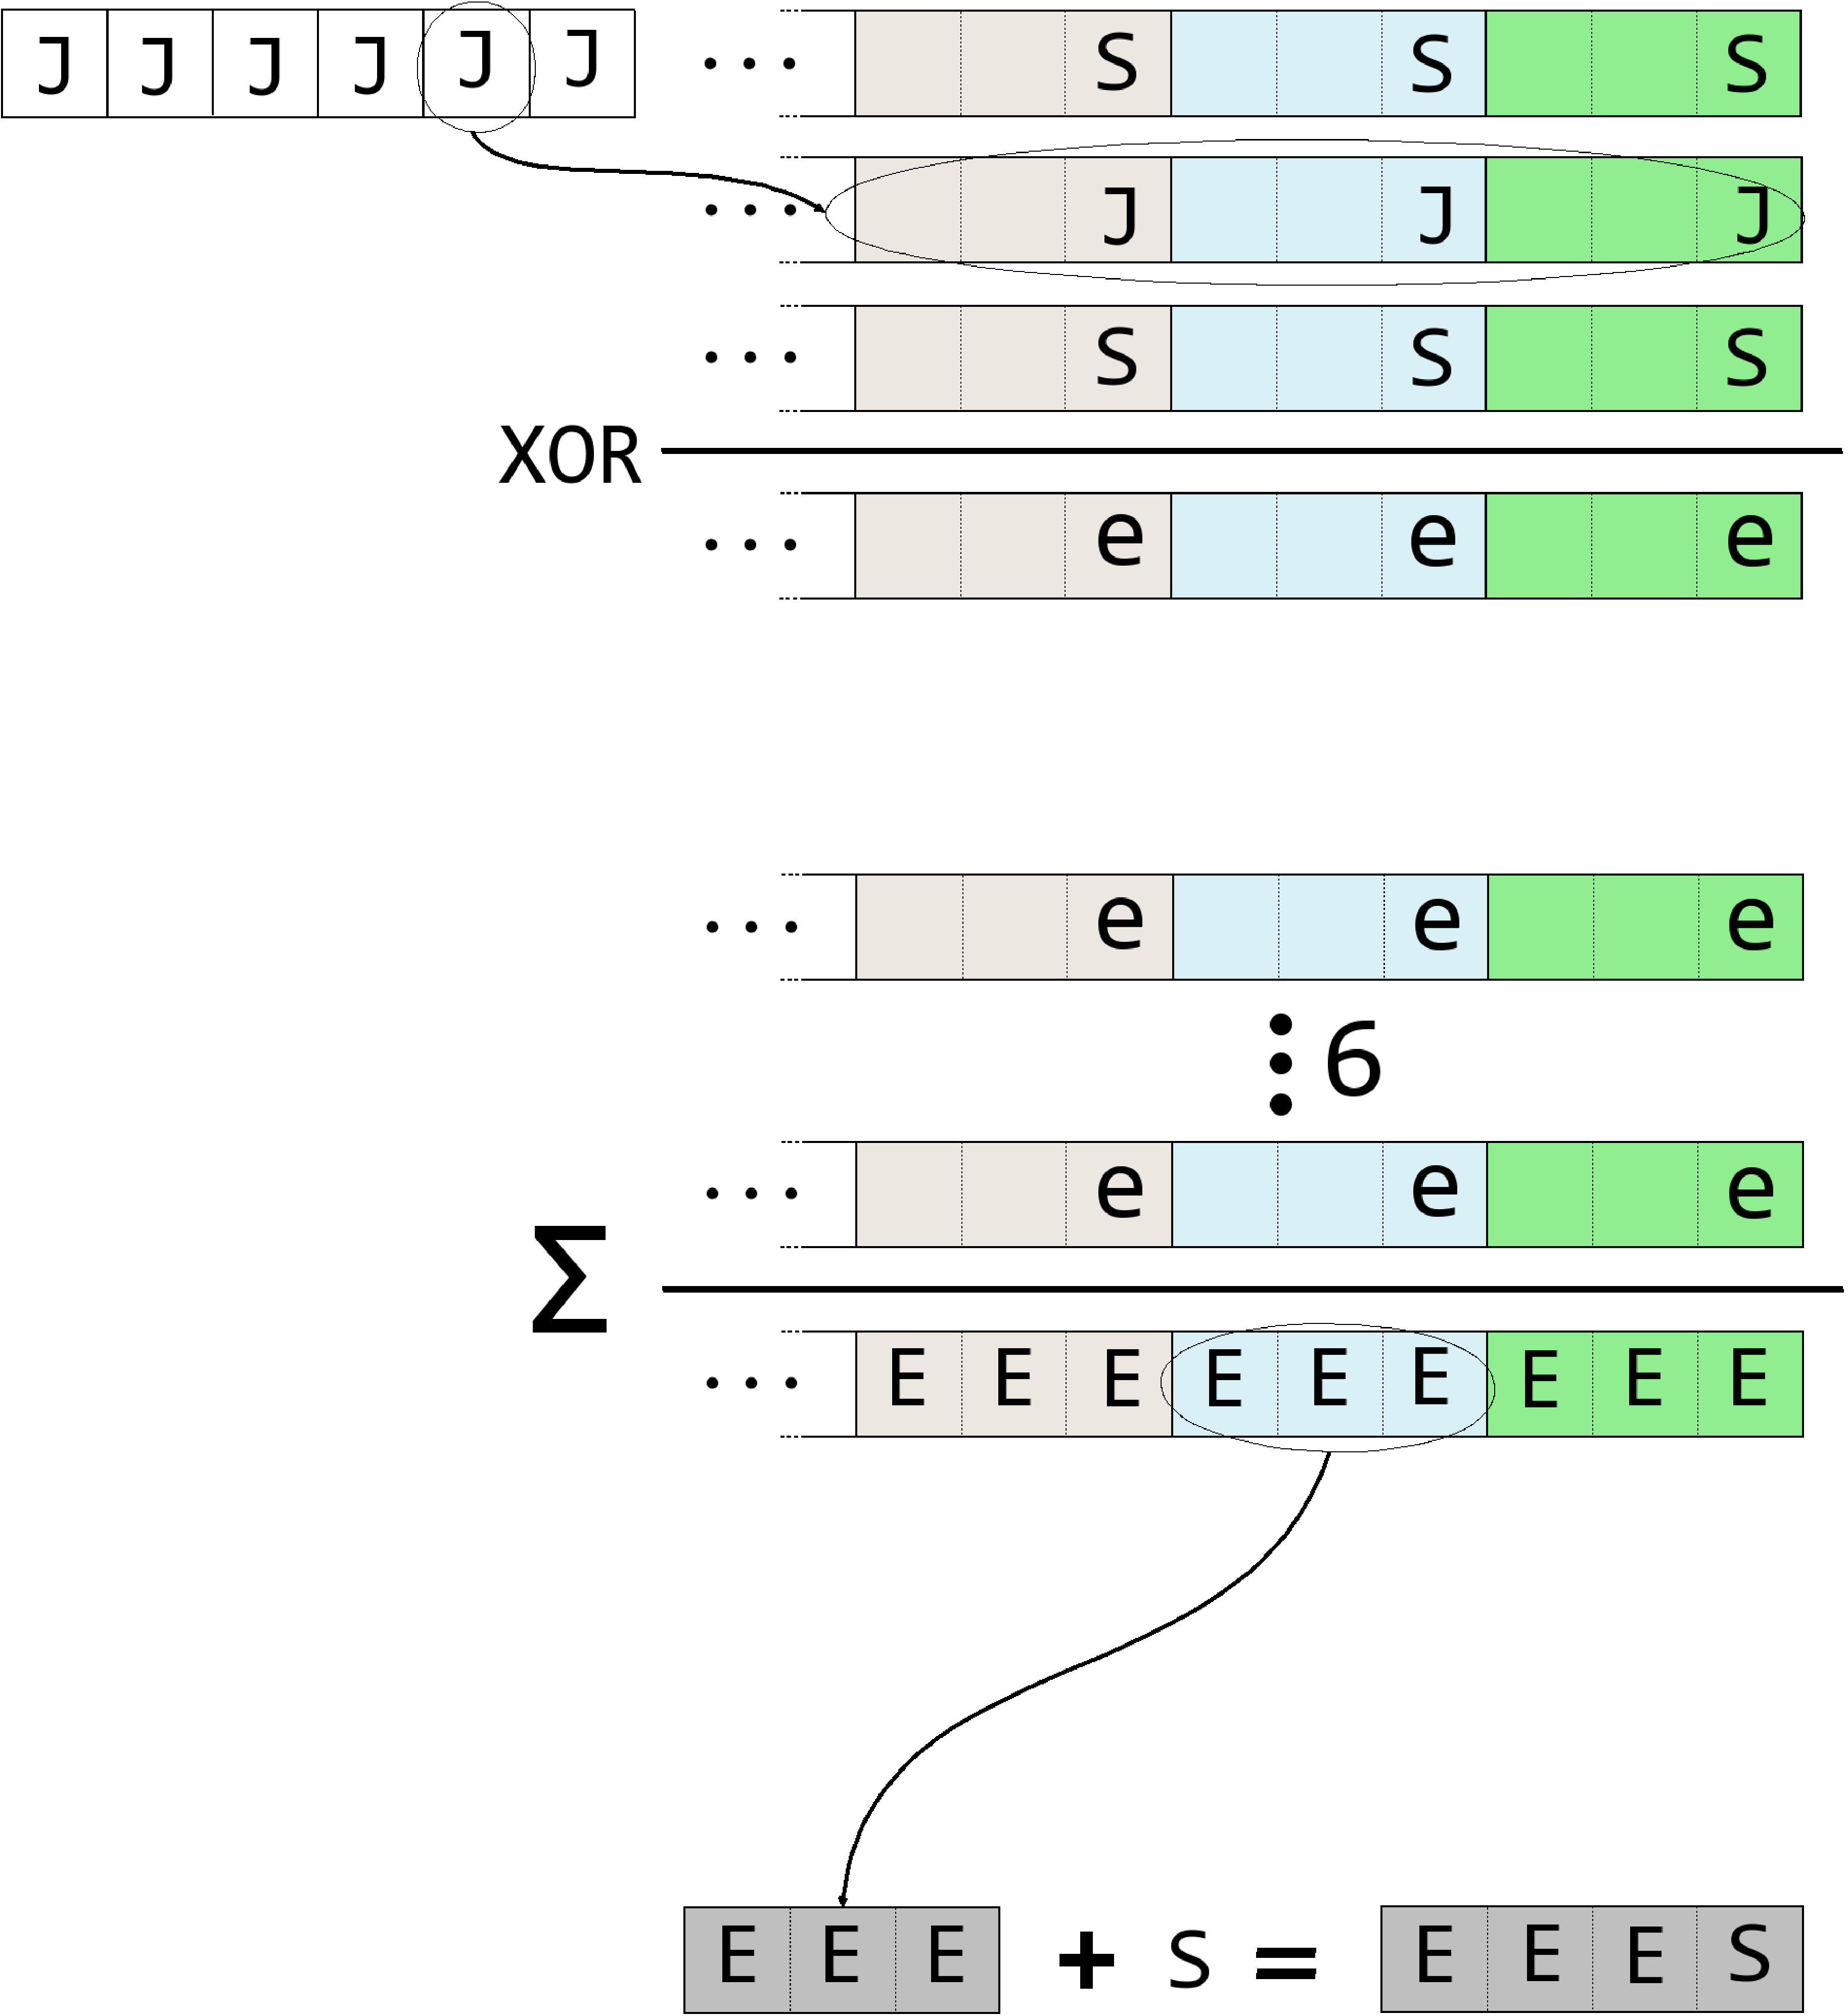
\includegraphics[width=0.31\textwidth]{../img/msc/new_amsc3.pdf}}\\
  \subfigure[AMSC1]{\includegraphics[width=0.4\textwidth]{img/new_amsc1.pdf}}\hspace{0.5cm}
  \subfigure[AMSC3]{\includegraphics[width=0.465\textwidth]{img/new_amsc3.pdf}}\\
\caption{This figure demonstrates the computation of $(E \times 2 +
  S)$ for the purpose of accessing the probability look up table with
  the deployment of two variations of Asynchronous Multispin Coding
  (AMSC).  Each line in the figure represents an integer, each box of
  a line represents a bit, and boxes of the same color represent a
  segment that hold a variable from one of the temperature replicas.
  We give the name AMSC1 and AMSC3 for these two AMSC schemes
  according to their segment width.  Unlike the AMSC1, the AMSC3
  scheme reserves three bits for each segment, and is a less dense
  storage format.  For the calculation of the local energy, we need
  two spins ($S$) and the coupling ($J$) between them. The $J$ bits
  and $S$ bits are integrated in the same integer, so that we can
  fetch both the coupling and the spins using only one memory
  transaction. The local energy ($e$) of each bond 
  can be calculated by performing two XOR operations. The
  total local change of energy ($EEE$) is the sum of the contributions
  from all six nearest neighbors. Since $EEE$ requires three bits for
  storage, the AMSC1 scheme compute each segment sequentially to
  avoid overflow, while the AMSC3 scheme can compute multiple segments in
  parallel.  After we obtain $EEE$ in three-bit format, we combine it
  with the spin state ($S$) by doing string concatenation.}
\label{fig_msc1}
\end{figure*}


\begin{figure*}
\centering
% \subfigure[AMSC4]{\includegraphics[width=0.284\textwidth]{../img/msc/new_amsc4.pdf}}\hspace{2.0cm}
% \subfigure[CAMSC]{\label{fig_camsc}\includegraphics[width=0.28\textwidth]{../img/msc/new_camsc.pdf}}
 \subfigure[AMSC4]{\includegraphics[width=0.426\textwidth]{img/new_amsc4.pdf}}\hspace{0.5cm}
 \subfigure[CAMSC]{\label{fig_camsc}\includegraphics[width=0.42\textwidth]{img/new_camsc.pdf}}
\caption{This figure demonstrates how the AMSC4 and CAMSC schemes help
  exploit bit-level parallelism in computing $(E \times 2 + S)$.
  Similar to that of the AMSC1 and AMSC3 (see the text and the caption
  of Fig.~\ref{fig_msc1}), the XOR operations and summation over six
  nearest neighbors produces the total local energy ($EEE$).  However,
  since we reserve four bits for each segment, and is capable of
  holding one more bit over $EEE$, the string concatenation of $EEE$
  with $S$ can now be vectorized.  The difference between CAMSC and
  AMSC4 is that $S$ and $J$ are stored in a more compact format. With
  such a design, CAMSC avoids waste of space and provides much better
  parallelism in computing $e$. }
  \label{fig_msc2}
\end{figure*}


We have briefly described the Multispin Coding (MSC). We have developed the 
Asynchronous Multispin coding (AMSC) as a more efficient
alternative to the conventional Synchronous Multispin Coding (SMSC)
for calculating the local energies ($E$), generating the 4 bit string
for the column index of the spin-flip probability table (section
\ref{section_prob}), and optimizing the memory bandwidth
utilization. In our particular GPU implementation, we use four byte
unsigned integers, which hold up to 32 bits, as a packed word. Each
spin, denoted as 0 or 1, takes only one bit of this packed word. Thus, the
calculations in Eq. \ref{eq:e} can be vectorized via bit-wise
operations. We integrate the $J$ bits with the $S$ bits in the same
integer, so that we can fetch both the coupling and the spins in only
one memory transaction. We then multiply the coupling with a bit-mask
to match the pattern of $S$, and calculate the bond energy with
bit-wise XOR operation. The next step is to add the six bond energies
around a spin to obtain the local energy.  To vectorize this process
we need to reserve empty bits to avoid overflow, since the local
energy takes 3 bits of storage. In this way, each spin, together with
the empty bits reserved for calculation, constitute a virtual segment.
%These 32 bits are conceptually partitioned into many segments.  
%Picking up each segment and compute sequentially is always feasible.  However, if the segment length is long 
%enough to cover the range of its resident, we can safely vectorize the computations (such as addition, 
%subtraction and bit-wise operations) for multiple segments.  
We derived three variations of AMSC with different segment width of 1, 3 and 4, denoted as 
AMSC1, AMSC3 and AMSC4 respectively. In AMSC1 and AMSC3, some calculations are 
sequentialized to avoid overflow. Figures \ref{fig_msc1} and \ref{fig_msc2} demonstrate how the  
the different variations of MSC parallelize the computations in Equations~\ref{eq:e}, \ref{eq:p} 
and~\ref{eq:r}. 

%Experiments(Figure \ref{fig_msc_perf}) confirm the effectiveness of AMSC,
%especially those with wider segments. 
Figure \ref{fig_msc_perf} illustrates that AMSC3 and AMSC4 are favored over AMSC1 due to improved 
overall performance.  However, we also observe proportionally longer times for
the memory transactions. %Meanwhile, the computational performance of AMSC4 does not improve much over AMSC3.
This demonstrates the limitation of the AMSC scheme: there does not exist an optimal segment width
that simultaneously provides the highest memory density, and the richest vectorization opportunities in computation.

%It is due to the fact that the effective memory density drops in proportion with the segment width, 
%and thus an increasing amount of memory transactions are required.
%increasingly amount of memory transactions that the effective memory density drops in proportion with the segment width.

To overcome the intrinsic limitation of AMSC, we propose a new scheme named Compact Asynchronous Multispin 
Coding (CAMSC).  We dynamically change the segment width to match the data range. % whenever profitable.
Longer width is adopted for larger data to qualify the vectorization of computing multiple segments. 
For small range data, we use shorter width to avoid blank bits reservations. 
For example, we allocate 1 bit per segment for $S$ and $e$, and then expand to 4 bits when calculating $E$. 
The segment width expansion is implemented with shift and mask operations. 
Figure \ref{fig_camsc} demonstrates the procedures of CAMSC and how it differs from traditional AMSCs.
Our experiment (Figure \ref{fig_msc_perf}) shows 28.4\% performance improvement 
when we switch from AMSC3 (46.8 ps/spin) to CAMSC (33.5 ps/spin).

% variable precision representation
% adapt the best segment width for values


\begin{figure}[!h]
  \centering
%  \includegraphics[width=0.45\textwidth]{../img/perf/percentage3b.pdf}
  \includegraphics[width=0.8\textwidth]{img/percentage3b.pdf}
  \caption{Comparing the performance using different multispin coding schemes. The experiment 
is done for a $16^3$ lattice, a shared memory probability table with integers and CURAND.
A parallel-tempering move is performed every 10 Metropolis single spin sweeps.}
  \label{fig_msc_perf}
\end{figure}






\section{Experimental Results}
\label{section_exp}

\subsection{The Platform Settings}
\label{section_platform}

Our development and performance evaluations are carried out on a
workstation with an Intel Core i7 x990 CPU and an NVIDIA GeForce GTX
580 GPU card. The GeForce GTX 580 is equipped with a Fermi architecture
GPU of 512 stream processors. We use Linux 2.6.32 x86-64, CUDA toolkit version 4.1
and gcc 4.4.6, and optimization flag -O2. We always configure the
GPU on-chip memory as 48KB shared memory plus 16KB L1 cache.

 
\subsection{Performance Evaluation}
\label{section_compare}
To evaluate the performance we use the time spent (in picoseconds) per spin flip proposal,
abbreviated as ps/spin (See eq. \ref{eq:tsf}).

When we study the equilibrium properties of a spin glass, the system
sizes that can be equilibrated within a reasonable time are not very
large. Therefore, we used $L=16$, or $N_\mathrm{spins}=4096$ as the
maximum system size. Meanwhile, to achieve efficient parallel
tempering moves, we set the number of temperature replicas to $N_T=24$ or $56$, 
and perform frequent parallel tempering moves (one parallel tempering move after
every $5$ to $10$ Monte Carlo sweeps). The typical number of Monte
Carlo steps required to equilibrate such a system is approximately
$10^7$.  Due to the huge sample-to-sample variation, a large number of
disorder realizations ($10^4$ or more) are usually required. However, since there is no
correlation among different realizations, we can scatter the jobs to
different GPU cards or nodes on a cluster.  On each of the cards we
only need $16$ to $64$ realizations to fully utilize all the
multiprocessors.

For benchmarking, we simulate 64 disorder realizations of the
EA model on a $16^3$ lattice with 24 temperature
replicas, and propose to swap adjacent temperatures every 10 Monte
Carlo sweeps.  We are able to complete $10^7$ Monte Carlo sweeps in 40 minutes. 
% the wall time speed is 38PS/s
% 38 * 10e-12 * (16 * 16 * 16 *  24 * 64 * 10e7 ) / 60 = 3984.5887999999995 minutes
This wall time consists of the single spin flip Monte Carlo time,
the parallel tempering swap time, and the measurement time.
Discarding the measurements, the average computational speed is 33.5
ps/spin, for a single GPU device.
% energy cost: 8.174 nJ/spin flip, given that maximum GPU power for a GTX 580 is 244W
If we simulate without parallel tempering and serve all
temperature replicas with the same random number, we could obtain 17.6
ps/spin.  Generating random numbers consumes about one third of the
total simulations time, as shown in Figure~\ref{fig_msc_perf}.  We
believe we are approaching the limit of performance optimization. For
reference, our single thread CPU code (using AMSC4 without parallel tempering on a $16^3$ cubic lattice) runs at the speed of 14737
ps/spin; this represents a speed up of almost 440 for the GPU code over
the CPU code.

Figure \ref{fig_perf} compares our implementation with similar
existing codes, where not all reference programs target at the
random frustrated Ising systems, present the external magnetic field, and feature parallel tempering.
Our program is substantially faster than any other GPU implementation
\cite{CSTN-093,2010CoPhC.181.1549B,doi:10.1142/S0129183112400025,Weigel:2012:PPS:2151219.2151631} for
small to intermediate system sizes. We are comparable to the
performance achieved by special-purpose FPGA
implementations\cite{2012arXiv1204.4134J}.


\begin{figure}[!ht]
  \centering
%  \includegraphics[width=0.5\textwidth]{../img/perf/compare.pdf}
  \includegraphics[width=0.8\textwidth]{img/compare.pdf}
  \caption{Performance comparison with other heterogeneous Ising model simulation programs.
\citet{CSTN-093} reports 4360.1 million Monte Carlo hits per second,
which equals to 229 ps/spin.
\citet{2010CoPhC.181.1549B} reports 7977.4 spin flips per microsecond,
which equals to 125 ps/spin.
}
  \label{fig_perf}
\end{figure}
 



\subsection{Simulation Results}
\label{section_result}

We test the code by simulating  both the simple ferromagnetic
Ising and the EA spin glass models.  In Figure
\ref{fig:energy-ising}, our results from the GPU code are found to be
consistent with the results from our CPU code for the ferromagnetic
Ising model, at various external magnetic fields. We also compare the
results with and without parallel tempering as a check to determine
whether the parallel tempering swap is performed correctly. We find
that the results with and without the parallel tempering swap are
consistent with each other. In Figure \ref{fig:corr-ising} we plot
the correlation length for the ferromagnetic Ising model in three
dimensions; here, the crossing point for the correlation length coincides
with the known critical temperature for the ferromagnetic
ordering. \cite{PhysRevB.44.5081}
For the EA model we calculate the Binder ratio
of the system at zero external magnetic field as shown in Figure
\ref{fig:binder-ea}. The results match reasonably well with the
published data. \cite{Katzgraber-Korner-Young-2006} Figure \ref{fig:qvst} demonstrates the effectiveness
of parallel tempering for the EA spin glass. The
parallel-tempering simulation reaches equilibrium after $10^5$ Monte
Carlo sweeps, while without parallel tempering, the system did not
reach equilibrium even with 100 times more iterations. This further
supports that we have implemented the parallel tempering swapping
correctly.

\begin{figure}[ht!]
 % \begin{minipage}[b]{0.45\textwidth}
    \centering
   % \includegraphics[width=0.5\textwidth]{../img/result/energy_compare.pdf}
    \includegraphics[width=0.8\textwidth]{img/energy_compare.pdf}
    \caption{Comparing the total energy of the $16^3$ sites Ising model with nearest neighbors coupling $J=-1$, to CPU generated results. At each value of 
      the external field, the GPU results are nearly identical to the CPU results. }
    \label{fig:energy-ising}
    \end{figure}
  %\end{minipage}

  %\begin{minipage}[b]{0.45\textwidth}
  \begin{figure}[ht!]
    \centering
%    \includegraphics[width=0.5\textwidth]{../img/result/ising_corr.pdf}
    \includegraphics[width=0.8\textwidth]{img/ising_corr.pdf}
    \caption{Correlation length vs.\ inverse temperature for the Ising model. The lines from different system sizes cross
    close to $1/T=0.2217$, which is in agreement with the published result for the critical temperature.~\cite{PhysRevB.44.5081}}
    \label{fig:corr-ising}
    \end{figure}
  %\end{minipage}

  %\begin{minipage}[b]{0.45\textwidth}
  \begin{figure}[ht!]
    \centering
   % \includegraphics[width=0.5\textwidth]{../img/result/binder_compare.pdf}
    \includegraphics[width=0.8\textwidth]{img/binder_compare.pdf}
    \caption{Binder Ratio for the 3D Edwards-Anderson model. The data generated by our GPU code is compared 
    with the data extracted from the paper by Katzgraber {\it et al.} \cite{Katzgraber-Korner-Young-2006}}
    \label{fig:binder-ea}
    \end{figure}
  %\end{minipage}

  %\begin{minipage}[b]{0.45\textwidth}
  \begin{figure}[ht!]
    \centering
    %\includegraphics[width=0.5\textwidth]{../img/result/qvst.pdf}
    \includegraphics[width=0.8\textwidth]{img/qvst.pdf}
    \caption{The convergence of the Binder ratio vs.\ number of Monte Carlo steps for the Edwards-Anderson
      model in a system with $8^3$ sites, 
    with and without parallel tempering for  $1/T=2.0$.  Parallel tempering dramatically improves 
    the convergence to equilibrium.}
    \label{fig:qvst}
    \end{figure}
  %\end{minipage}

%\end{figure}







\section{Conclusion and Future Works}

We design and implement a CUDA code for simulating the random frustrated
three-dimensional Edwards-Anderson Ising model on GPUs. 
For small to intermediate system sizes, our code runs faster than other
GPU implementations, and its speed is close to that of the specially built FPGA
computer. We note a very recent	preprint has reported an improvement in FPGA system. \cite{Janus2-2013}
Our performance tuning strategies include constructing three
levels (tasks, threads, bits) of parallel workloads for GPU;
optimizing the memory access via a proper data layout and tiling; 
speeding up the computation by translating time consuming floating point
operations to integer point operations and table look-ups; and finally,
vectorizing bit computations with our binary format, the Compact Asynchronous Multispin coding.

Our program can be extended for other models such as the Potts models and models with different random coupling distributions.
The structure of our code may adapt well to upcoming GPUs and future massive parallel accelerators.


\section*{Acknowledgments}

This work is sponsored by the NSF EPSCoR LA-SiGMA project under award number EPS-1003897. 
Portions of this research were conducted with high performance computational resources provided by 
Louisiana State University (http://www.hpc.lsu.edu).  Part of this work was done on the Oakley 
system at the Ohio Supercomputer Center. We thank Helmut Katzgraber and Karen Tomko for useful discussions. 
We thank the following collaborators: Bhupender Thakur, 
Ariane Papke, Sean Hall and Cade Thomasson. We thank Samuel Kellar for his careful reading of the manuscript.

%%% Local Variables:
%%% mode: latex
%%% TeX-master: "../thesis"
%%% End:

\chapter{Results for Three-Dimensional Edwards Anderson Model in 
an Externel Field}
\label{chap:sg_result}
This following chapter is a work titled {\bf Three Dimensional Edwards-Anderson 
Spin Glass Model in an External Field}, 
submitted for review to appear in Physics Review E.

In this paper, we discussed the results for Monte Carlo
Simulation of 3D Edwards-Anderson model.

This paper is written in collaboration with Ye Fang, Ka-Ming Tam, Zhifeng Yun, 
Juana Moreno, J. Ramanujam and Mark Jarrell. 

The idea of the project was first proposed by Ka-Ming Tam. 
Ye Fang and I developed the implementation together. With the code, I ran simulations
on the GPU clusters, accumulated and analyzed all the data. 

This paper is written in collaboration with Ye Fang, Ka-Ming Tam, Juana Moreno, 
and Mark Jarrell. I started a first draft, including the introduction, the 
simulation methods, the measured quantities and the conclusions. I also plotted 
all the figures from the data obtained in the simulation. 
Ka-Ming contributed to the introduction and conclusions. Juana Moreno
and Mark Jarrell also reviewed the paper and improved the conclusions.


\section{Introduction} 
Most spin systems order when the temperature is sufficiently low. 
Conventional magnetic orderings break the spin symmetry, and the moments align 
in a pattern with long range order. However, magnetic 
systems with random frustrated couplings can avoid conventional 
ordering by breaking ergodicity. Typical spin glass systems with 
such competing magnetic couplings include localized spins in metals coupled 
via the oscillating Rudermann-Kittel-Kasuya-Yosida 
exchange as CuFe and CuMn, and in insulators with competing interactions 
as in LiHoYF and EuSrS \cite{Binder-Young-1986,Mydosh-1993,Diep-2004}. These 
systems do not display long range order for a wide range of diluted spin 
concentrations.

A widely studied model to describe spin glass physics is the Edwards-Anderson 
(EA) model\cite{Edwards-Anderson1975}. It is composed of spins interacting
with their nearest neighbors via random couplings. The mean-field variant of the 
Edwards-Anderson model, the Sherrington-Kirkpatrick (SK) model\cite{Sherrington-Kirkpatrick1978,Sherrington-Kirkpatrick-1975},
was solved by the replica technique in 1975 with the striking observation that 
the entropy can be negative at low temperature\cite{Sherrington-Kirkpatrick-1975,Sherrington-Kirkpatrick1978}. 
A cavity mean field method was proposed by Thouless, Anderson 
and Palmer (TAP) in which the local magnetization of each site is considered as 
an independent order parameter\cite{Thouless-Anderson-Palmer-1977}. The hope was to 
obtain a more physical mean field solution without involving the replica technique. 
However, multiple solutions were found\cite{Bray-Moore-1980}.

Motivated by the deficits of previous approaches, de Almeida and Thouless
further studied the replica symmetric mean field solution and found a line 
in the temperature--magnetic field plane where the replica symmetry
solution is unstable towards replica symmetry breaking (RSB) \cite{Almedia-Thouless1978,Bray-Moore-1978}
The replica overlap has more structure than simply a constant. The way to 
characterize this structure for a stable mean field solution was developed 
by Parisi \cite{Parisi-1980a,Parisi-1980b,Parisi1980}.  There is a hierarchy 
of the replica overlap, and this can be described in terms of an ultra-metric tree. 
The replica symmetry breaking scheme resolved the negative entropy crisis and naturally 
explained the many solutions found in the TAP approach.

The replica symmetry breaking theory is accepted to be the correct description of the Sherrington-Kirkpatrick model; indeed 
it provides the exact free energy \cite{Talagrand-2006,Guerra-2003}. 
However, its applicability to low dimensional spin glass systems has been intensively debated 
over the last three decades, especially in the three dimensions case. For systems 
below the upper critical dimension \cite{Harris-Lubensky-Chen-1976,Tasaki-1989,Green-Moore-Bray-1983} 
the most prominent competing theory is the droplet model elaborated by 
Huse and Fisher \cite{Fisher-Huse-1988,Fisher-Huse-1987} and based on the idea of 
domain wall scaling by Moore, Bray and McMillan \cite{McMillan-1984,Bray-Moore-1987}. 
In this theory, there exists a finite characteristic length scale where droplets of 
excitations can lose energy by aligning with the field. The spin glass phase is thus 
destroyed by any finite external field. Moreover, those excitations are assumed to 
be compact and with fractal dimension smaller than the spacial dimension, in contrast 
with the space-filling excitations in the mean field theory. 

Thus a possible scheme to discern between the replica symmetry breaking and the droplet theories is to determine
whether a spin glass phase exists at a finite external field \cite{Young-Katzgraber2004}. 
There are other schemes based on the differences in the overlap and the excitations in these two theories. 
For example, the distribution of the overlap and the parameters that characterize it \cite{Hatano-Gubernatis-2002, 
Marinari-etal-1998,Marinari-etal-1999,Bokil-etal-1999,Moore-etal-1998,Monthus-Garel-2013}, 
the existence of the ultra-metric structure in the overlap \cite{Hed-Young-Domany-2004,Contucci-etal-2007}, 
and the nature of the ground state and its 
excitations \cite{Palassini-Young-2000a,Palassini-Young-2000b,Aspelmeier-Moore-Young-2003,Marinari-Parisi-2001,
Houdayer-Martin-1999,Marinari-Parisi-Zuliani-2000,Marinari-etal-1999}.
Unfortunately, the conclusions drawn from different studies are often controversial.  
This is mostly due to two factors, the limitation in the system sizes that can be 
simulated and the interpretation of the data. 

Using the same techniques on the three dimensional Edwards-Anderson model under an external field, no signal of 
a crossing of the scaled correlation length for different system sizes can be 
detected\cite{Young-Katzgraber2004}.  We will show this is also 
the case for the Binder ratio.  The absence of crossing is powerful evidence that a spin
glass phase is absent in the presence of an external field. However, it has been 
argued that the system sizes studied may be too small and far from the scaling 
regime. To remedy this problem, one dimensional models with long range power-law 
decaying interactions \cite{Kotliar-Anderson-Stein-1983} which mimic the short range models 
at higher dimensions have been intensively studied over the last few years \cite{Katzgraber-Young-2003a,Katzgraber-Young-2003b,
Leuzzi-1999}. In these models much larger systems can be studied \cite{Katzgraber-Larson-Young-2009,
Katzgraber-Hartmann-2009,Leuzzi-etal-2008,Larson-etal-2013}. It is worthwhile to mention that
the studies using Migdal-Kadanoff approximations for hierarchical lattice
tend to support the droplet picture \cite{Moore-Bokil-Drossel-1998,Migliorini-Berker-1998}. 

On top of these controversies, it has been recently argued that the scaled correlation length 
is not a good parameter for the spin glass transition in a field since its calculation involves 
the susceptibility at zero momentum \cite{Leuzzi-etal-2008}.
The latest proposal is to study the ratio of susceptibilities at the 
two smallest non-zero momenta, denoted it as $R_{12}$ \cite{Banos-2012}. It has 
been shown that in four dimensions this quantity displays a crossing
at finite temperature which is an important clue that the spin glass can still 
exist without time reversal symmetry below the upper critical dimension \cite{Banos-2012}. 
Giving the success of using $R_{12}$ to capture the spin glass phase
at four dimensions, we reexamine the three dimensional Edwards-Anderson model on a simple cubic lattice using 
a new development in computer architecture, and the recently proposed $R_{12}$. 
We will demonstrate that graphic card computing is particularly well suited for 
equilibrium simulations of spin glass systems, in particular for cases where a huge number 
of realizations is required such as the model we study in this work. 

The paper is organized as follows: The simulation methods and the quantities we measured 
are introduced in the Section II. In the section III, we show the data from our simulations.
We conclude our results and discuss the possible directions for the future study in the
section IV.


\section{Method and Measured Quantities} 
The Hamiltonian for the Edwards-Anderson model is given as
\begin{eqnarray}
H=-\sum_{<i,j>} J_{ij} S_{i}S_{j}-h\sum_{i}S_{i},
\label{Hamiltonian}
\end{eqnarray}
where $S_i$ indicates Ising spins on a simple cubic lattice with $N=L^3$ sites and periodic boundary conditions. 
The coupling $J_{ij}$ is bimodal distributed with probability %function 
$P(J_{ij}) = \frac{1}{2}(\delta(J_{ij}-1) + \delta(J_{ij}+1))$, and $h$ is an external field.

The spin glass overlap is defined as 
\begin{equation}
  \label{eq:overlap}
  q(\vec{k})=\frac{1}{N}\sum_{j}S_j^{(\alpha)} S_j^{(\beta)}\exp^{i\vec{k} \cdot \vec{r}_j},
\end{equation}
where $\alpha$ and $\beta$ are two independent realizations of the same disorder model.
We calculate the overlap kurtosis or the Binder ratio from the overlap as \cite{Ciria-etal-1993,Marinari-etal-1998}
\begin{equation}
  \label{eq:binder}
  g=\frac{1}{2}\left(3-\frac{\overline{\left<\left(q(0)-\overline{\left<q(0)\right>}\right)^4\right>}}{\overline{\left<\left(q(0)-\overline{\left<q(0)\right>}\right)^2\right>}^2}\right).
\end{equation}
Note that $\overline{(\cdots)}$ indicates averaging over different disorder realizations,
and $\left<\cdots\right>$ denotes thermal averaging.


The wave vector dependent spin glass susceptibility is defined as \cite{Marinari-etal-1998}
\begin{equation}
  \label{eq:chi}
  \chi(\vec{k})= N(\overline{\left<q^2(\vec{k})\right>}-\overline{\left<q(\vec{k})\right>}^2),
\end{equation}
and the correlation length as 
\begin{equation}
  \label{eq:corr}
  \xi_L=\frac{1}{2\sin(\vec{k}_{\mathrm{min}}/2)}\left[\frac{\chi(0)}{\chi(\vec{k}_{\mathrm{min}})}-1\right]^{1/2},
%\label{eq:corrlength}
\end{equation}
where $\vec{k}_{\mathrm{min}}=(2\pi/L,0,0)$. 

We define $R_{12}$ as the ratio between the susceptibilities with the two smallest non-zero wave 
vectors \cite{Banos-2012}
\begin{equation}
  \label{eq:r12}
  R_{12}=\frac{\chi(\vec{k}_1)}{\chi(\vec{k}_2)},
\end{equation}
where $\vec{k}_1=(2\pi/L,0,0)$, $\vec{k}_2=(2\pi/L,2\pi/L,0)$.


Parallel tempering\cite{Hukushima-Nemoto1996,Marinari-Parisi1992} is used to accelerate the thermalization, 
in which $N_T$ samples of the same disorder coupling are simulated in parallel within a range 
of temperatures. In order to compute 
the spin glass overlap (Eq.\ref{eq:overlap}) we simulate two replicas 
of the system with the same bonds $J_{ij}=\pm 1$ and field $h$ at each temperature. 

We implement the Monte Carlo simulation with parallel tempering on graphics 
processing units using the CUDA programming language \cite{Nickolls:2008:SPP:1365490.1365500}. 
Multispin coding\cite{PhysRevLett.42.1390,Zorn1981337} is used 
to pack the $N_T$ replicas into the small but extremely fast shared 
memory. We achieve a performance of 33ps per spin flip attempt on a GTX 580 card.
We use the CURAND implemented XORWOW generator to generate random numbers \cite{curand}.
Since the GPU is a commodity hardware and widely available in large
computer clusters, it is now easy to greatly accelerate these 
simulations. 
The details of the implementation can be found in 
Ref \cite{Fang-Feng-Tam-etal-2013}. 
%\cite{Zhang:2012:AAS:2259016.2259037,Weigel:2012:PPS:2151219.2151631,preis2011gpu,Preis:2009:GAM:1537305.1537344,Nguyen:2010:BOS:1884643.1884658,Micikevicius:2009:FDC:1513895.1513905,Maruyama:2011:PIP:2063384.2063398,doi:10.1142/S0129183112400025,DBLP:journals/ijpp/HawickLP11,CSTN-093,2012JCoPh.231.1209K,2012arXiv1204.6193M,2012arXiv1204.6192Y,2011CoPhC.182.1833W,2011arXiv1107.5463W,2010CoPhC.181.1549B,2010arXiv1006.2566B}


\begin{table}[ht]
  \centering
  \caption{Parameters of the simulations.  $L$ is the linear system size.
$N_{\mathrm{samp}}$ is the number of samples, 
$N_{\mathrm{sweep}}$ is the total number of Monte Carlo sweeps for each of the 2$N_T$ replicas 
for a single sample, $\beta_{\mathrm{max}}$ and $\beta_{\mathrm{min}}$ show the temperature 
region simulated, and $N_T$ is the number of temperatures used in the parallel tempering method. 
The temperature set in each simulation follows a geometric distribution, 
i.e. $\beta_n=\beta_{\rm min}\alpha^{n-1}$, where $\alpha=(\beta_{\rm max}/\beta_{\rm min})^{1/(N_T-1)}$, $n\in [1,N_T]$.
The first half of the Monte Carlo sweeps are used for thermalization and the second half are used for measurement.}
% \begin{ruledtabular}
 \begin{tabular}{lrrrrr}
    $L$&$N_{\mathrm{samp}}$&$N_{\mathrm{sweep}}$& $N_T$  &$\beta_{\mathrm{max}}$ &  $\beta_{\mathrm{min}}$  \\
\hline
%    4&190,000&2,000,000&24&2.0&0.7\\
6&500,000&2,000,000&56&1.8&0.1\\
8&350,000&2,000,000&56&1.8&0.1\\
10&240,000&2,000,000&56&1.8&0.1\\
%12&30,000&20,000,000&0.7&1.8&24\\
%16&30,000&20,000,000&0.7&1.5&24\\
  \end{tabular}
%\end{ruledtabular}
  \label{tab:parameters}
\end{table}

We list the parameters of our simulation in Table \ref{tab:parameters}. We 
benchmarked the code against existing results at $h=0$.  The smallest 
$\beta$ used in the parallel tempering is well below the critical temperature ($1/\beta_{c} = T_{c} \approx 1.1019 \pm 0.0029$) \cite{Baity-Jesi-etal-2013} of 
the spin glass transition at zero field\cite{PhysRevB.62.14237,Baity-Jesi-etal-2013}, while the largest $\beta$ 
is about two times larger.  The estimated critical field at zero temperature is around $h \approx 0.65$ for 
the model with zero mean and unit variance Gaussian distributed couplings\cite{Krzakala-etal-2001}. 
We choose to work in a relatively small field, $h=0.1$. 
%All the data we show use this strength of field. 
The jackknife method is used to estimate the statistical errors from disorder averaging. 



\section{Results} 
We plot the spin glass susceptibility in Fig. \ref{fig:Chi}. As in the 
zero field case, the susceptibility increases as the temperature is lowered, however there is
no obvious asymptotic scaling behavior. In particular, for temperatures below  
the zero-field critical temperature, the
slope of the curves decreases and they begin to bend downward. This result is similar to the one obtained for
the one dimensional model\cite{Larson-etal-2013}, but in contrast with the results of the four dimensional lattice 
which displays asymptotic divergent susceptibilities \cite{Marinari-etal-1998}.

\begin{figure}[ht]
\centering
  \includegraphics[width=0.6\textwidth]{img/chi.pdf}% 
  \caption{\label{fig:Chi} Spin glass susceptibility at zero momentum, $\chi(0)$, as a function of inverse temperature 
for system sizes $L=6,8,10$.}
\end{figure}


As the susceptibility does not show a behavior in accordance with the conventional 
finite size scaling theory for a second order transition, we move to study various 
cumulants and ratios of susceptibilities of the overlap parameter. We show the Binder ratio in Fig.~\ref{fig:Binder}. It does not display any signal of crossing. 
Indeed, the curves for different system sizes do not even tend to merge as the temperature 
is lowered.  Note that the Binder ratio corresponds to the fourth-order cumulant of the 
distribution, and 
%spin glass susceptibility at zero momentum. 
the possible issues related with the soft mode  
contributing to the zero momentum susceptibility should likely be canceled in the Binder ratio.

\begin{figure}[ht]
\centering

\centering
  \includegraphics[width=0.6\textwidth]{img/binder.pdf}% Here is how to import EPS art
  \caption{\label{fig:b-h0} Binder ratio as a function of inverse temperature in the
range  $\beta=0.1\sim1.8$ for system sizes $L=6,8,10$.}
\label{fig:Binder}
\end{figure}

Fig.~\ref{fig:c-h0} displays the scaled correlation length. This is now a standard 
diagnosis for the detection of a spin glass transition. The correlation length is 
extracted from the Ornstein-Zernike form (Eq.~\ref{eq:corr}), and thus essentially given by the ratio 
between the zero and the smallest finite momentum susceptibilities. 
Similar to the Binder ratio, and consistent with other results in the literature, 
there is no crossing or even merging down to a rather low temperature~\cite{Young-Katzgraber2004}.

\begin{figure}[ht]
\centering

  \includegraphics[width=0.6\textwidth]{img/corr.pdf}% Here is how to import EPS art
  \caption{\label{fig:c-h0} Scaled correlation length $\xi/L$ as a function of inverse temperature for system sizes $L=6,8,10$.  }
\end{figure}

From now on we focus on $R_{12}$. We performed simulations in zero field
where $R_{12}$ shows a crossing close to the expected critical temperature found from
the Binder ratio and the correlation. Therefore, the crossing in $R_{12}$ should 
be a viable indicator for the phase transition. Unfortunately, we find that $R_{12}$ is in 
general much noisier than other quantities. This is due to the fact that the sampling 
of higher momentum quantities is almost always characterized by larger statistical 
fluctuations. Taking the ratio between two susceptibilities at finite momenta clearly further
harms the quality of the data. To reduce the error bars we generate long runs and larger 
pools of disorder realizations (see Table \ref{tab:parameters}). This is the main reason we have generated a rather large number ($2.4 \times 10^5$) of realizations 
for the largest systems size we present here, and even more for smaller sizes. To further reduce the 
fluctuations, we impose all point group symmetries. For example, when we calculate 
$\chi(2\pi/L,0,0)$ we average the susceptibility at three different directions 
($\chi(2\pi/L,0,0)$, $\chi(0,2\pi/L,0)$, and $\chi(0,0,2\pi/L)$). This averaging implicitly assumes 
that the point group symmetry is restored which is justified only when the number of realizations
is rather large. 
 
\begin{figure}[ht]
\centering

\includegraphics[width=0.6\textwidth]{img/r12.pdf}% Here is how to import EPS art
\caption{\label{fig:r12} $R_{12}$ as a function of inverse temperature for different system sizes. 
An intersection can be seen at around $T \approx 0.6$. We use the jackknife method to estimate 
the error bar from sample-to-sample variation.  
}
\end{figure}

Fig.~\ref{fig:r12} displays $R_{12}$. In contrast to other quantities, $R_{12}$ shows an intersection 
at about $T \approx 0.6$. We do not think we have sufficient data to perform a reasonably accurate finite size 
scaling analysis to report the exponent or even to quantify the correction \cite{Hasenbusch-etal-2008}.
Moreover, the data for $L=6$ does not seem to fit into a finite size scaling form with the curve bending downward.
Unfortunately, parallel tempering Monte Carlo is not robust enough for simulating larger lattices in a reasonable 
amount of time; this can be related to the temperature chaos \cite{Ritort-1994,Fernandez-etal-2013,Katzgraber-etal-2007}. The number of replicas needed to equilibrate the system also 
increases substantially as the system size increases, we already used $56$ temperature 
replicas for $L=10$ simulations. We plot $R_{12}$ versus the number of Monte 
Carlo sweeps in Fig.~\ref{fig:MCsteps}. We believe the data is sufficiently equilibrated for averaged quantities.
The major contribution to the error is from the limited number of disorder realizations. Fig.~\ref{fig:R12_l10_samples} shows $R_{12}$ 
for $L=10$ for different numbers of realizations. We clearly see that the data converges only when the number of realizations is fairly large.
This is one of the prominent hurdles of using higher momentum susceptibility as a diagnosis. 
We note that the effective one dimensional model also shows crossing behavior,
albeit the crossing points do not show a systematic trend\cite{Larson-etal-2013}.


\begin{figure}[ht]
\centering

  \includegraphics[width=0.6\textwidth]{img/eq_l10.pdf}
  \caption{\label{fig:MCsteps} $R_{12}$ for $L=10$ at $\beta=1.8$, as a function of the 
number of Monte Carlo sweeps.  We believe the averaged data is equilibrated 
for $10^6$  sweeps, and it passes the logarithm binning 
test \cite{Alvarez-etal-2010}. The main contribution to the error is from the realization 
averaging.}
\end{figure}


\begin{figure}[ht]
\centering
  \includegraphics[width=0.6\textwidth]{img/R12_l10_samples.pdf}
  \caption{$R_{12}$ for $L=10$ and low temperatures ($\beta \geq 1.0$). We show five different numbers of 
realizations from fifteen thousand to two hundred forty thousand.}
\label{fig:R12_l10_samples}
\end{figure}


We studied the distribution of the susceptibilities. We calculated the susceptibility
for each disorder realization, and plotted the histogram at the lowest temperature,
$\beta=1.8$.
The distribution of susceptibilities are highly skewed. 
The mean of the distribution is dominated by rare
events, as suggested in Fig \ref{fig:hist_chi}. 
The non-Gaussian nature of the distribution suggests that the mean value might 
not be a good indicator. 


\begin{figure}[ht]
  \centering
  \includegraphics[width=0.7\textwidth]{img/chi_1_dist.pdf}
  \caption{Histogram for $\chi_1$ at low temperature.}
\label{fig:hist_chi}
\end{figure}

Here, we used the geometrical average \cite{PhysRevB.88.134204} over the susceptibilities to find $R_{12}$,
as shown in Fig \ref{fig:r12_gmean}.
We see that the lines are quite different from those obtained with arithmetic 
mean, and the crossings appear at different temperatures. 


\begin{figure}[ht]
  \centering
  \includegraphics[width=0.7\textwidth]{img/r12_gmean_h01.pdf}
\caption{\label{fig:r12_gmean} $R_{12}$ calculated from the geometrical average
of susceptibilities, 
as a function of inverse temperature, for different system sizes. 
}
\end{figure}


\section{Discussions and Conclusions}
In summary, we perform Monte Carlo simulations of the three-dimensional
Edwards-Anderson model in a finite external field. The goal is to reexamine the 
long-standing problem of whether mean field behavior, specifically a spin glass phase, can
exist in such a model without time-reversal symmetry. We focus on the equilibrium quantities
of this notoriously difficult system. By taking advantage of the new commodity multi-threaded 
graphic computing units architecture we drastically reduce the computation time. The results 
for the Binder ratio and correlation length for different cluster sizes show no signal of an 
intersection, thus they point to the absence of a spin glass transition
as found in  previous studies. On the other hand, the ratio of susceptibilities 
$R_{12}$ does show an intersection for relatively small system sizes ($L=6,8,10$). 
We did perform simulations for larger system sizes, but this data 
is too noisy in particular for $R_{12}$ to draw a conclusion.
With the present system sizes and the statistical error bar, a rigorous data 
analysis does not seem to deliver unbiased information. 
This situation is rather discouraging, as simulations at this low temperature 
for much larger system sizes using the present method are daunting. 
Although we can not reach a definitive conclusion on whether a spin glass phase 
transition exists under a finite magnetic field,
we showed that the susceptibilities are not normally distributed and mean is 
dominated by rare events.
This motivated us to study the geometric average of the distribution. 
We showed that for different system sizes, there is similar crossing behavior 
in the $R_{12}$ calculated from the geometric average. 


The results are obtained with a very small external field, $h=0.1$. It is possible
that a larger field, such as $h=0.25$, would give us a stronger signal of crossing.
While this may give us a slightly clearer signal on the phase transition, should 
the transition exist at h=0.25, it would likely occur at a significantly lower temperature
which further jeopardizes the quality of the simulation data. As the result stands now, 
we cannot find a clear phase transition in h=0.1, and if there were no phase transition, 
it would also rule out the possibility of the transition occurring in a larger field. 
On the other hand, if we found evidence for the absence of a transition at h=0.25, we 
cannot determine if the spin glass phase would survive a smaller field like h=0.1. 
There is no simple rule of thumb which can be used to determine what value of h is 
the best for the purpose of answering the question on the existence of the transition 
under an external magnetic field. But we believe that the possible advantage of using  
a larger field does not outweigh the disadvantages, both in term of the difficultly
of the simulation, and its predictive power. 

 
Due to our efficient GPU implementation, we were able to leverage the computing
power of supercomputing clusters with GPU accelerators, and study a large number of disorder
realizations.
Our results show that with current numerical methods and computing capability obtainable 
results are still not robust enough to provide dispositive insight into the nature 
of a spin glass in 3D, and that we need either a different method to study the 
distribution of the data, or an exponential increase in computing power to gain 
more knowledge for this problem. 
We also think that any previous research based on the susceptibilities may 
suffer from the same problem, and the results from these work may be improved
by including a much larger of samples.

%This calls for a more thorough study on the model with different approaches.
%Possible directions include: 1) using models with continuous random distribution which are 
%easier to thermalize than that with bimodal distribution; 2) analyzing the
%data for the distribution of the overlap parameter, instead of average quantities. 

We notice a preprint before
we finished the present paper where the conditioning variate method
is used to expose the silent features from the data \cite{Baity-Jesi-etal-2014}. 


%\appendix

\section{System with L=16}

We further tested with a bigger system size, $L=16$. We used 11,200 realizations,
and divide them into four batches, each containing 2800 samples. We then calculated
the $R_{12}$ for the four batches, and compared them, as shown in Fig \ref{fig:l16_r12}. 
The results shows that a few thousand realizations is not enough, even for a 
system size of L=16. 


\begin{figure}[ht]
  \centering
  \includegraphics[width=0.7\textwidth]{img/l16_r12.pdf}
  \caption{$R_{12}$ for a larger system with $L=16$. We used four batches of samples,
each batch contains 2800 disorder realizations. The results shows that for
different batches $R_{12}$ is quite different, especially at low temperatures.
}
\label{fig:l16_r12}
\end{figure}


This work is sponsored by the NSF EPSCoR Cooperative Agreement No. EPS-1003897 with additional support 
from the Louisiana Board of Regents. This research were conducted with high 
performance computational resources provided by 
Louisiana State University (http://www.hpc.lsu.edu). We thank Helmut Katzgraber and Karen 
Tomko for useful conversations. We thank the following collaborators: Bhupender Thakur, Ariane Papke, Sean Hall, and Cade Thomasson. 


%%% Local Variables:
%%% mode: latex
%%% TeX-master: "../thesis"
%%% End:


%%% Local Variables:
%%% mode: latex
%%% TeX-master: "../thesis"
%%% End:

\chapter{Strongly correlated materials}
\label{chap:cthyb}
\section{Introduction}

Many interesting phenomena in materials can be simply described in term
of a picture in which particles are independent of each others. For a periodic
system, Bloch's theorem provides the basis for the description of materials
in term of band structure. The energy eigenstates can be expanded in term
of the periodic function with definite momentum number. Even such a seemingly
simple independent particle picture harbors a vast amount of interesting phenomena.
Nine decades have passed after the Bloch's theorem, the physics of non-interacting electrons are
still being investigated intensively today. The exotic physics, such as 
the topological structure of the band theory still have not been exhausted,
typical examples include quantum hall effect and topological insulators.

Effects from the interaction among particles cannot be completely ignored in many
interesting systems. The physics can quickly become very complicated when
the interaction becomes a dominating factor in the system. Unlike the simple
single particle picture, there is no generic efficient method for the study 
of quantum interacting systems. From a computational point of view, the size
of the quantum system, Hilbert space, grows exponentially as the number of 
particles. It is in general very difficult to analyze such systems by simple numerical mean.

However if one can reduce the systems into a somewhat single particle like systems,
the analysis can be greatly simplified. The Landau Fermi liquid theorem, a landmark
achievement in the study of correlated systems, tells us that in many
circumstances the interacting system can be reduced into a single particle system with
some modifications. The non-interacting particle can be adiabatically deformed
into quasi-particle with a finite lifetime. This important prediction by Landau
can only be explained few decades later when the concepts of renormalization group
of fermion systems are applied in the condensed matter physics.

Although the Fermi liquid theorem can satisfactory explained a lot of metallic
systems, its limitation is obvious. It fails in the low-dimensional
cases, by now, we know that this is invalid in one dimension. However, the question 
of its validity in two dimensions is more subtle. As many of the interesting systems, their
physics are believed to be largely dictated by the correlation in two dimensions.
This is also the main battlefield of strongly correlated systems. In one dimension, 
various rather accurate numerical methods are available; in higher dimensions, 
mean field theory is presumably a good starting point. At two dimension, there is 
usually no good control on analytical calculations, and numerical methods for lattice
models are hindered by the minus sign problem in Quantum Monte Carlo or the lack
of good renormalization of the Hilbert space. Another clear deficit of the Fermi liquid 
theory is its inability to describe the quantum criticality, It is obvious that the 
criticality involves collective behaviors. An independent particle picture is 
doomed to fail in describing critical points. Further increase the interaction, 
the independent particle picture in the momentum space has to be replaced by the Mott 
picture in the real space, and there is no adiabatic continuation which can tune
the single particle metallic system into a real space picture of Mott insulator.

Thus, a systematic, even though approximated, method is sought for the study of strong correlation. 
The method which can describe the physics from metallic, to critical, to insulating phase as 
the interaction is cranked up is crucial for the study of strongly correlated systems. 
We will discuss in the following that the dynamical mean field method and its cluster extension, 
dynamical cluster approximation, fulfilled such a request. Combining with the density functional theory,
semi-quantitative numerical results can sometimes be obtained for strongly correlated materials. 


In a sense, from the above discussion, the term strong correlation refers to the behavior of electrons
that cannot be well-described by simple one-electron theories. Materials
which naturally have a tendency to strong correlation are those involved
unfilled d or f orbitals. This is due to the small orbital radius of
$d$ and $f$ orbitals and so does the overlap of orbitals.
This reduces the kinetic energy of the system, the electrons are said to be living 
in the narrow band, and thus the interaction becomes more important. Many interesting materials discovery which host
a range of interesting experimental observations, the most prominent example is the
high-temperature conductivity, pseudogap behaviors, quantum
criticality, in the past few decades involve transition
metal or inner transition metal. This is precisely because of the effective
strong correlation due to the $d$ or $f$ orbitals.

Understanding those exotic behaviors is extremely challenging. There is a major
obstacle. Once the single particle picture fails, there
is no good starting point for many perturbative calculations. It renders
into a regime almost all analytical methods will fail. In the following we 
will discuss two majors progress in attacking correlated systems. The first one 
is Density Functional Theory (DFT)\cite{PhysRev.136.B864,PhysRev.140.A1133} , 
a many-site single particle treatment; 
and the other one is Dynamical Mean Field Theory (DMFT) \cite{RevModPhys.68.13,PhysRevB.45.6479}, 
a single site many-body treatment. 

\section{Numerical approaches in strongly correlated materials}
Numerical calculation in strongly correlated fermion systems is a major 
challenge in condensed matter physics. In real world, materials consist of 
$10^{23}$ interacting particles, which is impossible to solve at first glance. 
Fortunately, not all the particles contribute to the property of materials. For 
example, in a metal only the electrons close to the Fermi level can be excited 
and contribute ,e.g., to the transport and magnetic properties. In a lattice, 
lattice excitations are few at low T, but they are responsible for inelastic 
neutron scattering. Even though, the remaining problem is still hard. 

Density functional theory (DFT)\cite{PhysRev.136.B864,PhysRev.140.A1133} 
provides a framework to solve the 
electron structure problem. Using this theory, the properties of a many-electron
system can be described by a functional of election density. Combined with 
approximations that address the exchange-correlations such as the local density 
approximation (LDA) \cite{lundqvist1983}, DFT produces satisfactory data that agrees well the 
experiments for many cases. However, despite the success in weakly correlated 
materials, there are still difficulties in applying this method to other 
cases, such as systems with strongly correlation \cite{0953-8984-9-35-010}. 
The accuracy of DFT has seen gradually improve over the year, the continual
development in functional to include correction from beyond local density 
plays an important part. However, it seems to be quite
difficult to handle such strong correlation by simple improvements of the 
DFT. A promising direction is to combine other methods which can treat
strong correlation with the DFT method. A popular choice is to employ 
the Dynamical Mean Field Theory\citep{RevModPhys.68.13,PhysRevB.45.6479} (DMFT)
to include the effect from the electron-electron
correlation on top of the single particle dispersion obtained from the DFT. 

%DFT, ab inito

%maybe mention other numerical methods here?

DMFT has been widely used on a range of strongly correlated systems. 
It is a method well suited for strongly correlated systems, in particular, it 
captures the Mott transition, a hallmark of strong correlation, of the Hubbard 
model. In this approach, the solution of the lattice model is mapped to a 
quantum impurity model with self-consistency conditions. 
%intro to impurity
%mention other impurity solvers
A quantum impurity problem describes an atom embedded in a host medium. 
The impurity consists of a set of orbitals with different parameters, populated
with electrons that interact with each other. The orbitals are hybridized to 
bath orbitals representing the degrees of freedom of the host materials. 
The solution of impurity problem can be obtained in a few different ways. 
We will focus on the different variants of Monte Carlo methods.

A commonly used technique is the Hirsch-Fye method \cite{1986PhRvL..56.2521H}, in which a 
Hubbard-Stratonovich transformation is used to decouple the interaction part,
leading to determinants which give the weights associated with the 
configurations of the auxiliary fields, which are then sampled by a Monte Carlo 
procedure. One issue is that Hirsch-Fye cannot be easily applied to complicated
interaction that includes more than just density-density interaction, due to the
lack of simple ansatz to decouple the interacting terms. 
The matrix size scales to the interaction as well as the inverse of 
temperature, which makes the calculation inefficient at low temperatures.
This method also requires discretization of the imaginary time interval,
which introduce systematic errors, and may not be optimal for the multi-orbital 
case with complicated off-diagonal couplings.

The Trotter error in Hirsch-Fye algorithm can be eliminated by using the 
Continuous Time Monte Carlo algorithms. For example, one can solve the problem 
exactly in non-interacting limit, and treat the interaction with a Taylor-series
 expansion. By doing stochastic sampling of diagrams in the weak-coupling 
expansion of partition function, the interaction expansion (CT-INT) algorithm
\cite{2005PhRvB..72c5122R}
provides a discretization error free alternative Hirsch-Fye algorithm.
Still, in the CT-INT algorithm, it is difficult to treat non-Hubbard-type 
interactions. Also, the size of the matrix used in the CT-INT method grows
quickly with the interaction, making the calculation very time-consuming at 
very strong interactions.

Another way to treat the impurity problem is the hybridization expansion (CT-HYB)
approach \cite{RevModPhys.83.349, PhysRevB.75.155113, PhysRevB.80.235117,
PhysRevB.74.155107}. 
The fact that the order of expansion decreases with increasing 
interaction makes this method favorable for strong interaction systems. 
The algorithm is also found to work at very low temperatures and is applicable
to a wider class of impurity models including those with complicated 
off-diagonal couplings since the local problem is treated exactly. 

\section{Algorithm}
\label{sec:hyb-alg}
\subsection{Hybridization Expansion CTQMC algorithm}
A quantum impurity model may be represented as a Hamiltonian $H_\text{QI}$

\begin{equation}
H_\text{QI}=H_\text{loc}+H_\text{bath}+H_\text{hyb}
\end{equation}
\begin{eqnarray}
H_\text{loc}&=& H_\text{loc}^0+H_\text{loc}^I=
                \sum_{ab} E^{ab}d^\dagger_a d_b + 
                \sum_{pqrs}I^{pqrs}d^\dagger_p d^\dagger_q d_r d_s \\
H_\text{bath}&=&\sum_{k\alpha} 
                 \varepsilon_{k\alpha}c^\dagger_{k\alpha}c_{k\alpha} \\
H_\text{hyb}&=&\sum_{k\alpha b} ({V}_k^{\alpha b}c^\dagger_{k\alpha}d_b 
                +\text{h.c.})
\end{eqnarray}

$H_\text{loc}$ describes the ``impurity'' (a system
with a finite (typically small) number of degrees of freedom), 
$H_\text{bath}$ describes the non-interacting system, 
and $H_\text{hyb}$ gives the coupling between the impurity and bath.

The Anderson impurity model describes a localized electronic level, subject to 
a local Coulomb interaction, which is coupled to a band of non-interacting 
conduction electrons. In the  single-impurity single-orbital case, its 
Hamiltonian is given by
\begin{equation}
H_\text{AIM}= \underbrace{\sum_{k\sigma}
  \varepsilon_k c^\dagger_{k\sigma}c_{k\sigma}}_{H_\text{bath}} 
+  \underbrace{\sum_\sigma \varepsilon_0d^\dagger_\sigma d_\sigma 
  + Un_\uparrow n_\downarrow}_{H_\text{loc}}
+ \underbrace{\sum_{k\sigma}\Big(V_kc^\dagger_{k\sigma}d_\sigma+h.c.\Big)}
_{H_\text{hyb}}
\end{equation}


In Hybridization Expansion Continuous Time Quantum Monte Carlo (CT-HYB)
\cite{RevModPhys.83.349,PhysRevB.75.155113,PhysRevB.80.235117,
PhysRevB.74.155107}, 
we take the hybridization term as a perturbation, i.e.
\begin{equation}
H_b=H_\text{hyb} = \sum_{pj} (V_p^j c_{p}^\dagger d_j
+ \sum_{pj} V_p^{j*}d_j^\dagger c_{p})
\end{equation}
and thus the partition function becomes
\begin{align}
Z &=\sum_{k=0}^\infty\int_0^\beta d\tau_1 \ldots \int_{\tau_{k-1}}^\beta d\tau_k 
    \int_0^\beta d\tau_1' \ldots  \int_{\tau_{k-1}'}^\beta d\tau_k' 
\sum_{\substack{j_1, \cdots j_k\\j_1', \cdots j_k'}}\sum_{\substack{p_1, \cdots p_k\\p_1',\cdots p_k'}} V^{j_1}_{p_1}V^{j_1'*}_{p_1'} \cdots V^{j_k}_{p_k}V^{j_k'*}_{p_k'}  \nonumber\\
&\times\Tr_d\left[T_\tau e^{-\beta H_\text{loc}} d_{j_k}(\tau_k) d_{j_k'}^\dagger(\tau_k')\cdots d_{j_1}(\tau_1)d_{j_1'}^\dagger(\tau_1')\right] \nonumber\\
&\times\Tr_c\left[T_\tau e^{-\beta H_\text{bath}} c^\dagger_{p_k}(\tau_k)c_{p_{k'}}(\tau_k')\cdots c_{p_1}^\dagger(\tau_1) c_{p_1'}(\tau_1')\right]
\end{align}
The bath partition function could be integrated out
\begin{align}
Z_\text{bath} = \Tr e^{-\beta H_\text{bath}} = \prod_\sigma \prod_{p} (1+e^{-\beta \varepsilon_{p}}),
\end{align}
With the anti-periodic hybridization function $\mathbf{\Delta}$,
\begin{align}
\Delta_{lm}(\tau) = \sum_p \frac{V^{l*}_p V^m_p}{e^{\varepsilon_p\beta}+1} \times 
\left\{ 
\begin{array}{ll}-e^{-\varepsilon_p(\tau-\beta)},& 0<\tau<\beta \\ 
e^{-\varepsilon_p\tau},&  -\beta<\tau<0\end{array}
\right.,
\end{align}
and by separating the contributions from each spin, we obtain
\begin{equation}
\label{partition_function}
Z =  Z_\text{bath}\prod_j \sum_{k_j=0}^\infty \int_0^\beta d\tau^j_1 \ldots \int_{{\tau'}^j_{k_j-1}}^\beta d{\tau'}^j_{k_j} 
\times \Tr_d\Big[T_\tau e^{-\beta H_\text{loc}} d_j(\tau^j_{k_j}) d_j^\dagger(\tau'^j_{k_j})\ldots d_j(\tau^j_{1})d_j^\dagger(\tau'^j_1)\Big] \det \mathbf{\Delta}_j
\end{equation}

Where 
\begin{equation}
  \label{eq:hyb-matrix}
  \Delta=\left[
    \begin{array}{cccc}
      \Delta(\tau_0'-\tau_0) & \Delta(\tau_0'-\tau_1) & \cdots & \Delta(\tau_0'-\tau_n)\\
      \Delta(\tau_1'-\tau_0) & \Delta(\tau_1'-\tau_1) & \cdots & \Delta(\tau_1'-\tau_n)\\
      \cdots & \cdots & \cdots & \cdots \\
      \Delta(\tau_n'-\tau_0) & \Delta(\tau_n'-\tau_1) & \cdots & \Delta(\tau_n'-\tau)\\
    \end{array}
  \right]
\end{equation}


We can sample the partition function above using Monte Carlo method. To 
determine the weight of each configuration, we need to calculate the contribution
from the local part (the trace) and the hybridization part (the determinant).
We would discuss both in the following sections \ref{sec:trace_segment},
\ref{sec:trace}, and introduce scalable 
algorithms in \ref{sec:cthyb_krylov} and \ref{sec:cthyb_fmu}.

\subsection{Evaluation of the trace using the segment picture}
\label{sec:trace_segment}
The trace factor represents the impurity with particles hopping in and out at 
imaginary times $\tau'$ and $\tau$, and the determinant sums up all compatible 
hybridization events with the bath. 
In the impurity basis ($\ket{0}$,$\ket{\uparrow}$,$\ket{\downarrow}$,
$\ket{\uparrow\downarrow}$) the Hubbard Hamiltonian is diagonal, 
and the creation and annihilation operators for given spin have to alternate 
for the trace to be finite. This allows the configuration of the operators to be
represented in a segment picture, where each pair of neighboring creation/annihilation 
operators are represented by a segment on the imaginary time axis, as shown in 
figure~\ref{fig:seg}.

%put segment picture here.
\begin{figure}[ht]
  \centering
  \includegraphics[width=0.8\textwidth] {img/segment.png}
  \caption{A segment picture showing a possible configuration of the two spin 
    channels. 
    The blue section indicates the overlap between two spin channels, 
    $l_\textrm{overlap}$ in eq.\ref{eq:weight_local}.}
\label{fig:seg}
\end{figure}


In the said basis, the contribution of the local Hamilton can be evaluated as:
\begin{equation}
\label{eq:weight_local}
W_{\textrm{loc}} = s_\uparrow s_\downarrow e ^{\mu(l_\uparrow+l_\downarrow)-Ul_{\textrm{overlap}}}
\end{equation}
Where $l_\sigma$ is the total length of segments on spin channel $\sigma$,
$l_{\textrm{overlap}}$ is the total overlap between two spin channels. The sign 
$s_\sigma$ is $-1$ when one of the segments winds around from $\beta$ to $0$, 
and $+1$ otherwise.

\subsection{Evaluation of the trace for non-diagonal Hamiltonian}
\label{sec:trace}
In models such as Dynamical Hubbard Model, the local part of Hamiltonian is not
diagonal in the occupation number basis, and, therefore, we cannot use the segment
picture to evaluate the trace easily. In this case, we need to evaluate the 
trace of this term:
\begin{equation}
  \label{eq:1}
  e^{-H*(\beta-t_n)}F_{t_n}e^{-H*(t_n-t_{n-1})}F_{t_{n-1}}\ldots F_{t_0}e^{-Ht_0}  
\end{equation}
Where $H$ is the Hamiltonian, and $F_{t_{i}}$ is a Fermion operator at time $t_i$.

To evaluate the exponential terms, we diagonalize the Hamiltonian with
\[
H=UVU^T
\]
where $V$ is a diagonal matrix with eigenvalues of $H$, each column of $U$ is an
eigenvector of $H$.
Using
\[
UU^T=I
\]
we have 
\[
e^{-Ht}=e^{-UVU^Tt}=Ue^{-Vt}U^T
\]
 the term becomes
\[
Ue^{-V*(\beta-t_n)}U^TF_{t_n}Ue^{-V*(t_n-t_{n-1})}\ldots F_{t_0}Ue^{-Vt_0}U^T
\]
define 
\[
D_t=U^TF_tU
\]
The term is then
\begin{equation}
  \label{eq:2}
  Ue^{-V*(\beta-t_n)}D_{t_n}e^{-V*(t_n-t_{n-1})}\ldots D_{t_0}e^{-Vt_0}U^T  
\end{equation}

We can then evaluate the full trace of the matrix above, using a series of 
matrix multiplications.


\subsection{Monte Carlo sampling}
\label{sec:cthyb_mcs}
To sample the configuration space with Monte Carlo procedures, one can propose 
a new configuration by:
\begin{itemize}
\item Adding a new segment to the existing configuration;
\item Removing a segment to the existing configuration;
\item Shifting an end of a segment in the existing configuration;
%\item Adding a new anti-segment to the existing configuration;
%\item Removing a anti-segment to the existing configuration;
\end{itemize}


To satisfy the detailed balance condition, we must make sure that 
\begin{equation}
W_{AB}/W_{BA}=W[B]W[A]
\end{equation}
where $A$ and $B$ are two configurations, and $W_{AB}$ is the transition
probability from configuration $A$ to configuration $B$, and vice versa.

In the case of adding a segment, one can first randomly choose a starting point 
for a segment, say $\tau'$ in $(\beta,0]$. If $\tau'$ falls on one of the 
existing segments, the proposal is rejected. Otherwise if $\tau'$ is located
between two segments $\tau_j$ and $\tau_{j+1}'$, we pick the end point from 
$[0,l_\textrm{max}]$, where 
$l_\textrm{max}=\mathrm{mod}(\tau_{j+1}'-\tau+\beta,\beta)$.
\begin{figure}[ht]
  \centering
  \includegraphics[width=0.8\textwidth] {img/segment.png}
  \includegraphics[width=0.8\textwidth] {img/segment_add.png}
  \caption{A segment picture showing the addition of a segment ($\tau_3',\tau_3$)
(red line) to the $\left|\downarrow\right\rangle$ channel. The red shade shows the
change of overlap from this addition.
}
\label{fig:seg_add}
\end{figure}
Assuming there is an infinitesimal grid with grid size $d\tau$ on the imaginary
time axis, the proposal probability can be found as:
\begin{equation}
P_\mathrm{prop:k\rightarrow k+1}=\frac{d\tau^2}{\beta\l_\mathrm{max}}
\end{equation}

\begin{figure}[ht]
  \centering
  \includegraphics[width=0.8\textwidth] {img/segment.png}
  \includegraphics[width=0.8\textwidth] {img/segment_remove.png}
  \caption{A segment picture showing the removal of a segment ($\tau_3',\tau_3$)
(red line) from the $\left|\uparrow\right\rangle$ channel.
}

\label{fig:seg_remove}
\end{figure}
In the case of removing a segment, one can randomly pick a segment from $k_\sigma$ 
existing segments, and thus the proposal probability is 
\begin{equation}
P_\mathrm{prop:k\rightarrow k-1}=\frac{1}{k_\sigma}
\end{equation}

Combined with the detailed balance condition and previous weight calculations, 
we have the probability of accepting an addition as:
\begin{equation}
P_\mathrm{accpt:k\rightarrow k+1}=\min\left(1,\mathrm{sign}(\tau-\tau')
  \frac{\beta l_\mathrm{max}}{k_\sigma +1} \frac{\det\Delta^{k+1}}{\det\Delta^k}
  e^{\mu l}e^{-U \Delta l_\mathrm{overlap}}
\right)
\end{equation}
where $l$ is the length of segment to be added, and $\Delta l_\mathrm{overlap}$
is the change in overlap between two spin channels. 

Similarly, the acceptance ratio for removing a segment is:
\begin{equation}
P_\mathrm{accpt:k\rightarrow k-1}=\min\left(1,\mathrm{sign}(\tau-\tau')
  \frac{k_\sigma}{\beta l_\mathrm{max}} \frac{\det\Delta^{k-1}}{\det\Delta^k}
  e^{-\mu l}e^{U \Delta l_\mathrm{overlap}}
\right)
\end{equation}

\begin{figure}[ht]
  \centering
  \includegraphics[width=0.8\textwidth] {img/segment.png}
  \includegraphics[width=0.8\textwidth] {img/segment_shift.png}
  \caption{A segment picture showing shifting the end of a segment ($\tau_1',\tau_1$)
(red line) on the $\left|\downarrow\right\rangle$ channel. The red shade shows the
change of overlap from this shift.
}

\label{fig:seg_shift}
\end{figure}

The probability for accepting a shifting move is:
\begin{equation}
P_\mathrm{accpt:k\rightarrow k}=\min\left(1,
  \mathrm{sign}(\tau_k-\tau_k')\mathrm{sign}(\tau_{k'}-\tau_{k'}')
  \frac{\det\Delta^{k}_{\mathrm{new}}}{\det\Delta^{k}}
  e^{\mu\Delta l}e^{-U \Delta l_\mathrm{overlap}}
\right)
\end{equation}

In the case where one or more channels have no segments, we need to evaluate the trace
from the Hamiltonian. Here $k$ refers to the number of segments on the channel
where the move is proposed, and $k'$ refers to the number of segments on the
channel with opposite spin direction.

\begin{enumerate}
  \item Adding a segment to channel $\sigma$.

    \begin{equation}
      P_\mathrm{accpt:k\rightarrow k+1}=\min\left(1,\mathrm{sign}(\tau-\tau')
        \frac{\beta l_\mathrm{max}}{k_\sigma +1} \frac{\det\Delta^{k+1}}{\det\Delta^k}
        *Q
      \right)
\end{equation}
where $Q$ is the ratio of the new trace verses the old trace. 

    \begin{enumerate}
    \item{$k=0,k'\neq 0$}

      \begin{equation}
        \label{eq:8}
        Q=
        \frac{e^{-l'_\sigma\epsilon_f}e^{-l_{ov}U}}
        {1+e^{-\beta\epsilon_f}e^{-l_{\bar\sigma} U}}
      \end{equation}
      Where $l'_\sigma$ is the length of the segment to be added, 
      $l_{ov}$ is the overlap between the new segment and the segments on channel $\bar\sigma$,
      and $l_{\bar{sigma}}$ is the total length of segments on channel $\bar\sigma$.

    \item{$k\neq 0,k'=0$}
      \begin{equation}
        \label{eq:9}
        Q=
        \frac{e^{-l'_{\sigma}\epsilon_f}(1+e^{-\beta\epsilon_f}e^{-(l_\sigma+l'_{\sigma})U)})}
        {1+e^{-\beta\epsilon_f}e^{-l_{\sigma} U}}
      \end{equation}
      Where $l'_\sigma$ is the length of the segment to be added, 
      and $l_{sigma}$ is the total length of segments on channel $\sigma$.
    
    
  \item{$k=0,k'=0$}
    \begin{equation}
        \label{eq:10}
        Q=
        \frac{e^{-l'_{\sigma}\epsilon_f}(1+e^{-\beta\epsilon_f}e^{-l'_{\sigma} U)})}
        {1+2e^{-\beta\epsilon_f}+e^{-\beta(2\epsilon_f+U)}}
      \end{equation}
      Where $l'_\sigma$ is the length of the segment to be added.
   
    \end{enumerate}

  \item Removing a segment.
    \begin{equation}
      P_\mathrm{accpt:k\rightarrow k-1}=\min\left(1,\mathrm{sign}(\tau-\tau')
        \frac{k_\sigma}{\beta l_\mathrm{max}} \frac{\det\Delta^{k-1}}{\det\Delta^k}
        *Q^{-1}
      \right)
    \end{equation}
    where $Q$ is calculated in Equations \ref{eq:8} $\sim$ \ref{eq:10}, in
    corresponding situations.
 
  \item Shift a segment.
    In the case of shifting, $k$ cannot be zero. Therefore the only special case
    is $k\neq 0, k'=0$. In this case,
    \begin{equation}
      \label{eq:9}
      Q=\frac{e^{-(l'_\sigma-l_\sigma)\epsilon_f}(1+e^{-\beta\epsilon_f}e^{-l'_\sigma U})}{1+e^{-\beta\epsilon_f}e^{-l_\sigma U}}
    \end{equation}
    Here $l_\sigma$ is the length of the chosen segment before the shift 
    operation, $l'_\sigma$ is the length after the operation.


 \end{enumerate}


When adding/removing/shift a segment on a channel, the hybridization matrix
needs to be updated accordingly.
\begin{enumerate}
\item Shifting

One can shift either the beginning or the end of a segment, which corresponds to
modifying a column/row in the hybridization matrix. For example, when shifting 
the end of segment $i$ from $\tau_i'$ to ${\tau_{new}'}$, the $i$th row of the matrix is updated:
\begin{equation}
  \small
  \label{eq:hyb-matrix-shift}
  \left[
    \begin{array}{cccc}
      \Delta(\tau_0'-\tau_0) & \Delta(\tau_0'-\tau_1) & \cdots & \Delta(\tau_0'-\tau_n)\\
      \Delta(\tau_1'-\tau_0) & \Delta(\tau_1'-\tau_1) & \cdots & \Delta(\tau_1'-\tau_n)\\
      \cdots & \cdots & \cdots & \cdots \\
      \Delta(\tau_i'-\tau_0) & \Delta(\tau_i'-\tau_1) & \cdots & \Delta(\tau_i'-\tau_n)\\
      \cdots & \cdots & \cdots & \cdots \\
      \Delta(\tau_n'-\tau_0) & \Delta(\tau_n'-\tau_1) & \cdots & \Delta(\tau_n'-\tau)\\
    \end{array}
  \right]\\
\Rightarrow
  \left[
    \begin{array}{cccc}
      \Delta(\tau_0'-\tau_0) & \Delta(\tau_0'-\tau_1) & \cdots & \Delta(\tau_0'-\tau_n)\\
      \Delta(\tau_1'-\tau_0) & \Delta(\tau_1'-\tau_1) & \cdots & \Delta(\tau_1'-\tau_n)\\
      \cdots & \cdots & \cdots & \cdots \\
      \textcolor{red}{\Delta({\tau_{new}'}-\tau_0)} & \textcolor{red}{\Delta({\tau_{new}'}-\tau_1)} & \textcolor{red}{\cdots} & \textcolor{red}{\Delta(\tau_{new}'-\tau_n)}\\
      \cdots & \cdots & \cdots & \cdots \\
      \Delta(\tau_n'-\tau_0) & \Delta(\tau_n'-\tau_1) & \cdots & \Delta(\tau_n'-\tau)\\
    \end{array}
  \right]
\end{equation}

\item Adding
Adding a segment $(\tau,\tau')$ between the original $i-1$ and $i$th segment 
corresponds to adding a row and column in the hybridization matrix. 
\begin{equation}
\small
  \label{eq:hyb-matrix-add}
  \left[
    \begin{array}{cccccccc}
      \Delta(\tau_0'-\tau_0) & \Delta(\tau_0'-\tau_1) & \cdots & \Delta(\tau_0'-\tau_{i-1}) &\textcolor{red}{\Delta(\tau_0'-\tau)} & \Delta(\tau_0'-\tau_i)&\cdots & \Delta(\tau_0'-\tau_n)\\
      \Delta(\tau_1'-\tau_0) & \Delta(\tau_1'-\tau_1) & \cdots & \Delta(\tau_1'-\tau_{i-1}) &\textcolor{red}{\Delta(\tau_1'-\tau)} & \Delta(\tau_1'-\tau_i)&\cdots & \Delta(\tau_1'-\tau_n)\\
      \cdots & \cdots & \cdots & \cdots  & \textcolor{red}{\cdots} & \cdots & \cdots & \cdots\\
      \Delta(\tau_{i-1}'-\tau_0) & \Delta(\tau_{i-1}'-\tau_1) & \cdots & \Delta(\tau_{i-1}'-\tau_{i-1}) &\textcolor{red}{\Delta(\tau_{i-1}'-\tau)} & \Delta(\tau_{i-1}'-\tau_i)&\cdots & \Delta(\tau_{i-1}'-\tau_n)\\
      \textcolor{red}{\Delta(\tau'-\tau_0)} &\textcolor{red}{\Delta(\tau'-\tau_1)} & \textcolor{red}{\cdots} & \textcolor{red}{\Delta(\tau'-\tau_{i-1})} &\textcolor{red}{\Delta(\tau'-\tau)} & \textcolor{red}{\Delta(\tau'-\tau_i)}&\textcolor{red}{\cdots} & \textcolor{red}{\Delta(\tau'-\tau_n)}\\
      \Delta(\tau_i'-\tau_0) & \Delta(\tau_i'-\tau_1) & \cdots & \Delta(\tau_i'-\tau_{i-1}) &\textcolor{red}{\Delta(\tau_i'-\tau)} & \Delta(\tau_i'-\tau_i)&\cdots & \Delta(\tau_i'-\tau_n)\\
      \cdots & \cdots & \cdots & \cdots  & \textcolor{red}{\cdots} & \cdots & \cdots & \cdots\\
      \Delta(\tau_n'-\tau_0) & \Delta(\tau_n'-\tau_1) & \cdots & \Delta(\tau_n'-\tau_{i-1}) &\textcolor{red}{\Delta(\tau_n'-\tau)} & \Delta(\tau_n'-\tau_i)&\cdots & \Delta(\tau_n'-\tau_n)\\
    \end{array}
  \right]\end{equation}

\item Removing
Removing a segment $(\tau_i,\tau_i')$ also removes the corresponding row and 
column in the hybridization matrix. 

\end{enumerate}
 
\section{Measurement}
\label{sec:cthyb_measurement}
\subsection{Single Particle Green's Function}
The imaginary time green's function can be found by:
\[
G(\tau)=-\left\langle\frac{1}{\beta}\sum_{ij}^k
\left(\Delta^{(k)}\right)^{-1}_{ji}\delta(\tau,\tau_i'-\tau_j)\right\rangle_{MC}
=-\left\langle\frac{1}{\beta}\sum_{ij}^k
M^{(k)}_{ji}\delta(\tau,\tau_i'-\tau_j)\right\rangle_{MC}
\]
To reduce noise and save memory, we split $\beta$ in to fine grids \verb|N_TAU| 
and bin data. 

We can also find the Matsubara frequency Green's function by 
Fourier transform:
\[
G(i\omega)=-\langle\frac{1}{\beta}\sum_{i,j}\exp^{i\omega(\tau_j'-\tau_j)}M_{ji}\rangle_{MC}
\]

Note that for a small number of \verb|N_TAU|,
the Fourier transform back to Matsubara frequency may be inaccurate. 

%When compiling, define \verb|-DMEASURE_GIO| to enable this measurement.

\subsection{Susceptibilities}

The charge susceptibility is defined 
\begin{equation}
  \label{eq:chi-charge}
  \chi_\mathrm{c}(\tau)=\left\langle[n_\uparrow+n_\downarrow](\tau)  [n_\uparrow+n_\downarrow](0)\right\rangle=\frac{1}{\beta}\int_0^\beta d\tau_0[n_\uparrow+n_\downarrow](\tau+\tau_0)  [n_\uparrow+n_\downarrow](\tau_0)
\end{equation}
Here $[n_\uparrow+n_\downarrow](\tau)$ stands for $n_\uparrow+n_\downarrow$ 
at the imaginary time $\tau$.

The spin susceptibility is defined 
\begin{equation}
  \label{eq:chi-spin}
  \chi_\sigma(\tau)=\left\langle[n_\uparrow-n_\downarrow](\tau)  [n_\uparrow-n_\downarrow](0)\right\rangle=\frac{1}{\beta}\int_0^\beta d\tau_0[n_\uparrow-n_\downarrow](\tau+\tau_0)  [n_\uparrow-n_\downarrow](\tau_0)
\end{equation}

In CY-HYB, the terms can be easily evaluated by shifting all of the segments on one
channel, and measure the overlap between the shifted channel and the other channel.



\section{DMFT Loop}

A commonly used method to solve lattice problems is to use the Dynamical Mean
Field Theory (DMFT) to approximate the original problem by an impurity problem
plus a self-consistency condition.

The impurity problem is solved by the 
CT-HYB impurity solver described above, and an impurity Green's function 
$G_f(i\omega)$
is obtained. The impurity Green's function is used to produce the lattice
Green's function $\mathcal{G}(i\omega)$ by the coarse-graining process.
The impurity Green's function and the lattice Green's function should obey 
Dyson's equation:
\begin{equation}
  \label{eq:3}
  G_f(i\omega)=\frac{1}{\mathcal{G}^{-1}(i\omega)+\Sigma(k,i\omega)}
\end{equation}

For next-neighbor hopping $t_∗$ on the Bethe lattice with density of states 
\begin{equation}
  \label{eq:bethe_dos}
  \rho_{Bethe}(\epsilon)=\left\{
    \begin{array}{ll}
      \frac{\sqrt{4t_*^2-\epsilon^2}}{2\pi t_*^2}&\mathrm{for} |\epsilon|\leq 2|t∗|  \\
      0&\mathrm{otherwise}
    \end{array}
  \right.
\end{equation}
,
the self-consistency equation yields a simple relation
\begin{equation}
  \label{eq:5}
  \mathcal{G}(i\omega)=i\omega+\mu-t_*^2G_f(i\omega)
\end{equation}
or 
\begin{equation}
  \label{eq:6}
  \Delta(i\omega)=t_*^2G_f(i\omega)
\end{equation}

This also allows us to do the Fourier transform from Matsubara frequency to imaginary
time easily. 

Overall, the DMFT loop is implemented as following:
\begin{enumerate}
\item Initialize the hybridization function $\Delta(\tau)$.
\item Call the impurity solver and get $G_f(i\omega)$.
\item Obtain the new hybridization function by $\Delta'(i\omega)=t_*^2G_f(i\omega)$
\item Linearly mix the new hybridization function with the old 
  by 
  \begin{equation}
    \label{eq:7}
    \Delta(i\omega) = m * \Delta'(i\omega)+ (1-m) \Delta_\mathrm{old}(i\omega)    
  \end{equation}
\item Fourier transform $\Delta(i\omega)$ to $\Delta(\tau)$.
\item Goto 2, and iterate till converge.

\end{enumerate}

\begin{figure}
  \centering
\smartdiagramset{%
 circular distance=30mm,
 text width=20mm,
 module minimum width=20mm,
 module minimum height=20mm,
 module shape=diamond,
 arrow tip=to,
 uniform arrow color=true,
 arrow color=gray!50!black,
 border color=black,
 uniform color list=white for 6 items, % new key to make colors uniform easily
% circular final arrow disabled=true, % new key to remove the final arrow
 additions={
   additional item offset=15mm,
   additional item shape=circle,
   additional item border color=black,
   additional item shadow=drop shadow,
   additional arrow color=gray!50!black,
 }
}
\smartdiagramadd[circular diagram]{$\Delta(i\omega)$,$\Delta(\tau)$, $G_f(i\omega)$, Converge?}
{left of module2/Start,right of module4/End}
\smartdiagramconnect{-to}{additional-module1/module2}
\smartdiagramconnect{-to}{module4/additional-module2}
  \caption{A diagram for the DMFT loop.}
\end{figure}

\section{Implementation}
\label{ssec:hyb-implementation}
We implement an impurity solver based the CT-HYB algorithm for 
Intel Many Integrated Core Architecture, or Intel MIC. Intel MIC is an 
x86-compatible multiprocessor architecture that can utilize existing 
parallelization software tools, such as OpenMP, OpenCL, etc. The x86 
compatibility makes it easy to execute the program on coprocessor with little
code modification. The Xeon Phi 7120P is capable of 1.2 teraFLOPS of double 
precision floating point instructions with 352 GB/sec memory bandwidth at 300W.
The current top supercomputer on TOP500 list, Tianhe-2, uses Intel Ivy Bridge
processors and Xeon Phi coprocessors to achieve 33.86 petaFLOPS.

\subsection{OpenMP parallelization}
We use a straightforward OpenMP approach to parallelizing our code. By deploying
multiple Markov chains on each processor/coprocessor, we have an embarrassingly 
parallel program, where each of the processes is independent of another, thus, no
communication overhead is required. Next, we discuss how we speed up the 
computation and optimize our performance. 

\subsection{Fast Matrix Update}
\label{sec:cthyb_fmu}
The most time-consuming part of the algorithm is the update of the hybridization
matrix. For each proposed update, the determinant of the new matrix is required
to compute the accepting probability. A straight forward determinant computation
scales to $k^3$, where $k$ is the expansion order. Due to the fact that in each
update move, only one row and one column are changed, one can use the 
Sherman-Morrison formula to update the matrix determinant and the inverse 
matrix in $k^2$, thus making the update process much more efficient, especially 
at low temperatures.

Suppose $\mathbf A$ is an invertible square matrix, and $\vec{u}$ and $\vec{v}$
are column vectors that describe the update to the matrix, then the determinant
of the new matrix is
\begin{equation}
\det({\mathbf A}+\vec{u}\vec{v}^T)=(1+\vec{v}^T\vec{A}^{-1}\vec{u})\det(\vec{A})
\end{equation}
To update the inverse of the matrix, one can use
\begin{equation}
(\vec{A}+\vec{u}\vec{v}^T)^{-1}=\vec{A}^{-1}-
\frac{\vec{A}^{-1}\vec{u}\vec{v}\vec{A}^{-1}}{1+\vec{v}^T\vec{A}^{-1}\vec{u}}
\end{equation}

In practice, the update of the inverse includes a few more steps, such as 
inserting/removing empty rows/columns, to ensure the size of the matrix 
reflects the change in the number of segments. Each Monte Carlo move requires two
updates to the matrix and its inverse, one for the column, and one for the row.

With the vectorization on Intel CPUs and MIC coprocessors, this procedure can 
be done efficiently on both platforms.

%\subsubsection{Update rows and columns}

%\subsubsection{Adding/removing rows and columns}

\subsection{Krylov method}
\label{sec:cthyb_krylov}
When the Hamiltonian is not diagonal, the update of the trace can be very expensive.
 The complexity of the method described in \ref{sec:trace}
 is $O(m^3n)$, where $m$ is the size of the 
matrix, and $n$ is the number of fermion operators in the series. Since $m$ 
scales exponentially with the number of orbitals, this can be 
very expensive even for a moderate number of orbitals (say 5). Instead, we can 
use the Krylov method\cite{PhysRevB.80.235117} to find the trace.

First, we find the few lowest eigenstates of the Hamiltonian $|i\rangle$, since 
they are usually more relevant at low temperatures. Then the trace is 
approximately
\[
\sum_i\langle i|  e^{-H*(\beta-t_n)}F_{t_n}e^{-H*(t_n-t_{n-1})}F_{t_{n-1}}
\ldots F_{t_0}e^{-Ht_0}  |i\rangle
\]

Then each of the term in the summation become of a series of the following 
operations:
\begin{itemize}
\item $e^{-Ht}|v\rangle$
\item $F|v\rangle$
\end{itemize}

The second operation is $O(m^2)$, so we'll ignore it for now. For the first term,
we can generate a Krylov space using the following method: 
%\footnote{ANALYSIS OF SOME KRYLOV SUBSPACE APPROXIMATIONS TO THE MATRIX 
%EXPONENTIAL OPERATOR, Y. SAAD , section 2.1}
\begin{enumerate}
\item $v_1=v/||v||$,
\item Iteration: do $j=1,2,\ldots,k$ 
  \begin{enumerate}
  \item $w=Hv_j$
  \item Iteration: do $i=1,2...,j$
    \begin{enumerate}
    \item $h_{i,j}=w\cdot v_i$
    \item $w=w-h_{i,j}v_i$
    \end{enumerate}
  \item  $h_{j+1,j}=||w||$, $v_{j+1}=w/h_{j+1,j}$
  \end{enumerate}

\end{enumerate}

With these iteration, we generate a orthonormal basis 
$V_k=[v_1,v_2,\ldots, v_k]$
and a $k\times k$ matrix $H_k$, where $H_k(i,j)=h_{i,j}$.

The exponential term can be just evaluated by:
\[
e^{-Ht}v \approx ||v|| V_m e^{-H_k t}e_1
\]
where $e_1 = [1, 0, 0, \ldots 0]^T$ . 

The complexity of this operation is $O(k^3+mk^2+m^2k)$. Usually a small value ($\sim 3$)
of $k$ is needed, thus, the complexity of the computation is reduced. 
Overall the complexity scales as $O(m^2kn)$.


\subsection{Using Legendre Polynomials}

To reduce high-frequency noise in the measurements of Green's function, 
one can use a set of Legendre polynomials\citep{2011PhRvB..84g5145B} as basis and measure the coefficients. 
%See arxiv:1104.3215.
\[
G_l=\sqrt{2l+1}\int_0^\beta d\tau P_l(x(\tau))G(\tau)
\]

In CTHYB:
\[
G_l=-\frac{\sqrt{2l+1}}{\beta}\left\langle\sum_{ij}M_{ji}\tilde{P}_l(\tau_i'-\tau_j)\right\rangle_{MC}
\]
Where
\[
\tilde{P}(\tau)=\left\{
\begin{array}{ll}
  P_l(x(\tau))& \tau >0\\
  -P_l(x(\tau+\beta))&\tau<0
\end{array}
\right.
\]
and \[
x(\tau)=2\tau/\beta-1
\]

To restore $G(\tau)$ or $G(i\omega)$ from the measured set of coefficients,
\[
G(\tau) = \sum_{l\ge 0}\frac{\sqrt{2l+1}}{\beta}P_l(x(\tau))G_l
\]
and
\[
G(i\omega) = \sum_{l\ge 0} G_l\frac{\sqrt{2l+1}}{\beta}\int_0^\beta\exp^{i\omega_n\tau}P_l(x(\tau))=\sum_{l\ge 0}T_{nl}G_l
\]
Where
\[
T_{nl}=(-1)^ni^{l+1}\sqrt{2l+1}j_l\left(\frac{(2n+1)\pi}{2}\right)
\]
and $j_l(z)$ are spherical Bessel functions. Note that in the procedure, no model-guided Fourier transform is used.

By setting an appropriate cut-off at the number of Legendre series, high-frequency noise is filtered. 
One can measure the error in the Legendre polynomials to determine where the cutoff should be.
%TRIQS used 80. 

%When compiling the code, use \verb|-DMEASURE_LEG| to enable this measurement.



\subsection{Optimization}
We use Intel Vtune Amplifier to benchmark the code and identify the bottlenecks.
The Intel Vtune Amplifier provides a set of performance insight into CPU and
Xeon Phi performance, threading performance, etc. We use Command Line Interface (CLI)
of Intel Vtune Amplifier, and inspected metrics such as:
\begin{itemize}
\item Walltime of application
\item Hotspot, tells the time consumption 
\item Cycles per instruction, or CPI rate %, tells the average number of CPU cycles 
%required to retire an instruction, and therefore is an indicator of how much latency 
%in the system affected the running application;
\item L1 Hit Ratio
\item Estimated Latency Impact
\item Vectorization Intensity
\item L1 Compute to Data Access Ratio
\item L2 Compute to Data Access Ratio
\end{itemize}

Several techniques are used to eliminate the bottlenecks and improve overall
performance, including:
\begin{itemize}
\item Random number generators
    The Monte Carlo sampling technique we use requires multiple random numbers 
generated on each thread with every update step, and we use pseudo-random generators (random number generator)
to produce them. 

  The most commonly used random number generator in C is the \texttt{rand()} function, which 
returns a pseudo-random integer using a hidden state. The \texttt{srand()} set 
its argument as the seed for a new sequence of pseudo-random number to be returned
by \texttt{rand()}. The function rand() is not thread-safe, since the hidden 
state it uses is modified on each call. When called from multiple threads,
this cause congestion, and the performance penalty is even worse for a massively 
parallel platform like Xeon Phi comparing to CPUs.

In order to get thread-safe behavior in
our multi-threaded application, we can use the function \texttt{rand\_r()}. Unlike
\texttt{rand()}, \texttt{rand\_r()} uses a pointer to an unsigned int to store state
between calls, so each different thread can use its own state. 
Therefore, \texttt{rand()} calls should be replaced with thread-safe \texttt{rand\_r()}
to avoid performance penalty and ensure code correctness.

\begin{figure}
  \centering
  \includegraphics[width=0.8\textwidth] {img/mic/perf_rand_r.png}
  \caption{Performance using different random number generators.}
\end{figure}

  We also tested other more advanced random number generators in our code, such as Mersenne Twister, 
and PCG. They offer better statistical quality in the pseudo-random number sequence,
and also have great multi-threading efficiency. However, the overall performance
gain is not significant, since the thread-safe random number generator itself is not very time consuming
comparing to other parts of the code. 

\item Move memory allocation out of the OpenMP region
 In our implementation, the hybridization matrix needs to be updated for each 
accepted Monte Carlo move, and the size of the matrix depends on the number of 
segments in each channel. In addition to the old and updated matrices, temporary
storage for the intermediate matrices used in the fast update process are also
required. 

We find that the repeated allocation and free of memory used for the
said matrices poses a huge performance penalty. A better practice would be 
allocating all the space for the matrices before the OpenMP region, and free 
after the threads join. This sets a limit on the max size of the matrices. For
a low temperature, more segments are expected, which means the size of the matrices
would be bigger, and thus a larger space needs to be assigned. 

\begin{figure}
  \centering
  \includegraphics[width=0.8\textwidth] {img/mic/memory.png}
  \caption{Performance before and after memory allocation optimization for MIC.}
\end{figure}


\item Improve data access pattern in kernel by
\begin{itemize}
  \item Separating loops to avoid cache bank conflict
  \item Interchanging loops to guarantee Unit-Stride Access
  \item Aligning elements in array
  \item Enhancing matrix storage
\end{itemize}
\end{itemize}
With these optimization methods, we improved CPI rate, L1 hit ratio, and 
vectorization intensity. We achieved more than two times speedup comparing to 
original CPU code.


%\section{Dynamic Hubbard Models}
%\label{ssec:hyb-mod}

\section{Preliminary results}
We benchmark our CTQMC solver with another Hirsch-Fye code and compare the results,
as shown in Fig.\ref{fig:u2}. This verifies that we can match the results of 
other impurity solvers.

\begin{figure}
  \centering
  \label{fig:u2}
  \includegraphics[width=0.8\textwidth] {img/U=2.png}
  \caption{Results for $G(\tau)$ on Anderson Model, from our code comparing with
weak coupling results.
Here $\beta = 50, U = 2, \mu = −1, v^2 = 0.156, D = 1, \Delta = v^2(log(i\omega + D) − log(i\omega − D))$}
\end{figure}



\section{Discussion\label{sec:hyb-concl}}

Although the formalism shown in \ref{sec:hyb-alg} is derived for single 
impurity Anderson model, the CT-HYB algorithm can be extended to more orbitals,
or other models easily, by changing the $H_\textrm{loc}$ term in the Hamiltonian 
and treating the term exactly. For example, we can easily extend the code to two or more
orbitals, and use exact diagonalization to calculate the contribution of the 
local term. For more orbitals, a Krylov solver\cite{PhysRevB.80.235117} can be used to reduce the cost of
trace computation, as discussed in section \ref{sec:cthyb_krylov}.

One of the possible application of the solver is the Dynamical Hubbard Models. 
The Dynamical Hubbard models contain the idea of break the electron-hole 
symmetry, due to the insufficiency of conventional Hubbard model in describing 
some scenarios in real materials, where important physics happens in transport 
and other processes. With the new methods applied, we hope one can answer the question 
about superconductivity in the dynamical Hubbard model. 

%%% Local Variables:
%%% mode: latex
%%% TeX-master: "../thesis"
%%% End:

%\chapter{Hybridization Expansion Continuous Time Quantum Monte
Carlo Solver}% and Application on Dynamic Hubbard Models

\label{sec:hyb}
\section{Algorithm}
\label{sec:hyb-alg}
\subsection{Hybridization Expansion CTQMC algorithm}
A quantum impurity model may be represented as a Hamiltonian $H_\text{QI}$

\begin{equation}
H_\text{QI}=H_\text{loc}+H_\text{bath}+H_\text{hyb}
\end{equation}
\begin{eqnarray}
H_\text{loc}&=& H_\text{loc}^0+H_\text{loc}^I=
                \sum_{ab} E^{ab}d^\dagger_a d_b + 
                \sum_{pqrs}I^{pqrs}d^\dagger_p d^\dagger_q d_r d_s \\
H_\text{bath}&=&\sum_{k\alpha} 
                 \varepsilon_{k\alpha}c^\dagger_{k\alpha}c_{k\alpha} \\
H_\text{hyb}&=&\sum_{k\alpha b} ({V}_k^{\alpha b}c^\dagger_{k\alpha}d_b 
                +\text{h.c.})
\end{eqnarray}

$H_\text{loc}$ describes the ``impurity'' (a system
with a finite (typically small) number of degrees of freedom), 
$H_\text{bath}$ describes the non-interacting system, 
and $H_\text{hyb}$ gives the coupling between the impurity and bath.

The Anderson impurity model describes a localized electronic level, subject to 
a local Coulomb interaction, which is coupled to a band of non-interacting 
conduction electrons. In the  single-impurity single-orbital case, its 
Hamiltonian is given by
\begin{equation}
H_\text{AIM}= \underbrace{\sum_{k\sigma}
  \varepsilon_k c^\dagger_{k\sigma}c_{k\sigma}}_{H_\text{bath}} 
+  \underbrace{\sum_\sigma \varepsilon_0d^\dagger_\sigma d_\sigma 
  + Un_\uparrow n_\downarrow}_{H_\text{loc}}
+ \underbrace{\sum_{k\sigma}\Big(V_kc^\dagger_{k\sigma}d_\sigma+h.c.\Big)}
_{H_\text{hyb}}
\end{equation}


In Hybridization Expansion Continuous Time Quantum Monte Carlo (CT-HYB)
\cite{RevModPhys.83.349,PhysRevB.75.155113,PhysRevB.80.235117,
PhysRevB.74.155107}, 
we take the hybridization term as a perturbation, i.e.
\begin{equation}
H_b=H_\text{hyb} = \sum_{pj} (V_p^j c_{p}^\dagger d_j
+ \sum_{pj} V_p^{j*}d_j^\dagger c_{p})
\end{equation}
and thus the partition function becomes
\begin{align}
Z &=\sum_{k=0}^\infty\int_0^\beta d\tau_1 \ldots \int_{\tau_{k-1}}^\beta d\tau_k 
    \int_0^\beta d\tau_1' \ldots  \int_{\tau_{k-1}'}^\beta d\tau_k' 
\sum_{\substack{j_1, \cdots j_k\\j_1', \cdots j_k'}}\sum_{\substack{p_1, \cdots p_k\\p_1',\cdots p_k'}} V^{j_1}_{p_1}V^{j_1'*}_{p_1'} \cdots V^{j_k}_{p_k}V^{j_k'*}_{p_k'}  \nonumber\\
&\times\Tr_d\left[T_\tau e^{-\beta H_\text{loc}} d_{j_k}(\tau_k) d_{j_k'}^\dagger(\tau_k')\cdots d_{j_1}(\tau_1)d_{j_1'}^\dagger(\tau_1')\right] \nonumber\\
&\times\Tr_c\left[T_\tau e^{-\beta H_\text{bath}} c^\dagger_{p_k}(\tau_k)c_{p_{k'}}(\tau_k')\cdots c_{p_1}^\dagger(\tau_1) c_{p_1'}(\tau_1')\right]
\end{align}
The bath partition function could be integrated out
\begin{align}
Z_\text{bath} = \Tr e^{-\beta H_\text{bath}} = \prod_\sigma \prod_{p} (1+e^{-\beta \varepsilon_{p}}),
\end{align}
With the anti-periodic hybridization function $\mathbf{\Delta}$,
\begin{align}
\Delta_{lm}(\tau) = \sum_p \frac{V^{l*}_p V^m_p}{e^{\varepsilon_p\beta}+1} \times 
\left\{ 
\begin{array}{ll}-e^{-\varepsilon_p(\tau-\beta)},& 0<\tau<\beta \\ 
e^{-\varepsilon_p\tau},&  -\beta<\tau<0\end{array}
\right.,
\end{align}
and by separating the contributions from each spin, we obtain
\begin{equation}
\label{partition_function}
Z =  Z_\text{bath}\prod_j \sum_{k_j=0}^\infty \int_0^\beta d\tau^j_1 \ldots \int_{{\tau'}^j_{k_j-1}}^\beta d{\tau'}^j_{k_j} 
\times \Tr_d\Big[T_\tau e^{-\beta H_\text{loc}} d_j(\tau^j_{k_j}) d_j^\dagger(\tau'^j_{k_j})\ldots d_j(\tau^j_{1})d_j^\dagger(\tau'^j_1)\Big] \det \mathbf{\Delta}_j
\end{equation}

We can sample the partition function above using Monte Carlo method. To 
determine the weight of each configuration, we need to calculate the contribution
from the local part (the trace) and the hybridization part (the determinant).
We would discuss both in the following sections \ref{sec:trace_segment},
\ref{sec:trace},\ref{sec:hyb_matrix}, and introduce scalable 
algorithms in \ref{sec:cthyb_krylov} and \ref{sec:cthyb_fmu}

\subsection{Evaluation of the trace using the segment picture}
\label{sec:trace_segment}
The trace factor represents the impurity with particles hopping in and out at 
imaginary times $\tau'$ and $\tau$, and the determinant sums up all compatible 
hybridization events with the bath. 
In the impurity basis ($\ket{0}$,$\ket{\uparrow}$,$\ket{\downarrow}$,
$\ket{\uparrow\downarrow}$) the Hubbard Hamiltonian is diagonal, 
and the creation and annihilation operators for given spin have to alternate 
for the trace to be finite. This allows the configuration of the operators to be
represented in a segment picture, where each pair of neighboring creation/annihilation 
operators is represented by a segments on the imaginary time axis, as shown in 
figure~\ref{fig:seg}.

%put segment picture here.
\begin{figure}[ht]
  \centering
  \includegraphics[width=0.8\textwidth] {img/segment.png}
  \caption{A segment picture showing a possible configuration of the two spin 
    channels. 
    The blue section indicates the overlap between two spin channels, 
    $l_\textrm{overlap}$ in eq.\ref{eq:weight_local}.}
\label{fig:seg}
\end{figure}


In the said basis, the contribution of the local Hamilton can be evaluated as:
\begin{equation}
\label{eq:weight_local}
W_{\textrm{loc}} = s_\uparrow s_\downarrow e ^{\mu(l_\uparrow+l_\downarrow)-Ul_{\textrm{overlap}}}
\end{equation}
Where $l_\sigma$ is the total length of segments on spin channel $\sigma$,
$l_{\textrm{overlap}}$ is the total overlap between two spin channels. The sign 
$s_\sigma$ is $-1$ when one of the segments winds around from $\beta$ to $0$, 
and $+1$ otherwise.

\subsection{Evaluation of the trace for non-diagonal Hamiltonian}
\label{sec:trace}
In models such as Dynamical Hubbard Model, the local part of Hamiltonian is not
diagonal in the occupation number basis, and therefore we cannot use the segment
picture to evaluate the trace easily. In this case We need to evaluate the 
trace of this term:
\begin{equation}
  \label{eq:1}
  e^{-H*(\beta-t_n)}F_{t_n}e^{-H*(t_n-t_{n-1})}F_{t_{n-1}}\ldots F_{t_0}e^{-Ht_0}  
\end{equation}
Where $H$ is the Hamiltonian, and $F_{t_{i}}$ is a Fermion operator at time $t_i$.

To evaluate the exponential terms, we diagonalize the Hamiltonian with
\[
H=UVU^T
\]
where $V$ is diagonal matrix with eigenvalues of $H$, each column of $U$ is a
eigenvector of $H$.
Using
\[
UU^T=I
\]
we have 
\[
e^{-Ht}=e^{-UVU^Tt}=Ue^{-Vt}U^T
\]
 the term becomes
\[
Ue^{-V*(\beta-t_n)}U^TF_{t_n}Ue^{-V*(t_n-t_{n-1})}\ldots F_{t_0}Ue^{-Vt_0}U^T
\]
define 
\[
D_t=U^TF_tU
\]
The term is then
\begin{equation}
  \label{eq:2}
  Ue^{-V*(\beta-t_n)}D_{t_n}e^{-V*(t_n-t_{n-1})}\ldots D_{t_0}e^{-Vt_0}U^T  
\end{equation}

We can then evaluate the full trace of the matrix above, using a series of 
matrix multiplications.


\subsection{The hybridization matrix}
\label{sec:hyb_matrix}
The contribution of the hybridization part can be calculated from the 
determinant of the hybridization matrix. 
\begin{equation}
  \label{eq:4}
  \Delta=\left[
    \begin{array}{cccc}
      \Delta(\tau_0'-\tau_0)& \Delta(\tau_1'-\tau_1) & \cdots& \Delta
    \end{array}


  \right]
\end{equation}

\subsection{Monte Carlo sampling}
\label{sec:cthyb_mcs}
To sample the configuration space with Monte Carlo procedures, one can propose 
a new configuration by:
\begin{itemize}
\item Adding a new segment to the existing configuration;
\item Removing a segment to the existing configuration;
\item Shifting an end of a segment in the existing configuration;
%\item Adding a new anti-segment to the existing configuration;
%\item Removing a anti-segment to the existing configuration;
\end{itemize}


To satisfy the detailed balance condition, we must make sure that 
\begin{equation}
W_{AB}/W_{BA}=W[B]W[A]
\end{equation}
where $A$ and $B$ are two configurations, and $W_{AB}$ is the transition
probability from configuration $A$ to configuration $B$, and vice versa.

In the case of adding a segment, one can first randomly choose a starting point 
for a segment, say $\tau'$ in $(\beta,0]$. If $\tau'$ falls on one of the 
existing segments, the proposal is rejected. Otherwise if $\tau'$ is located
between two segments $\tau_j$ and $\tau_{j+1}'$, we pick the end point from 
$[0,l_\textrm{max}]$, where $l_\textrm{max}=\mathrm{mod}(\tau_{j+1}'-\tau+\beta,\beta)$.
\begin{figure}[ht]
  \centering
  \includegraphics[width=0.8\textwidth] {img/segment.png}
  \includegraphics[width=0.8\textwidth] {img/segment_add.png}
  \caption{A segment picture showing the addition of a segment ($\tau_3',\tau_3$)
(red line) to the $\left|\downarrow\right\rangle$ channel. The red shade shows the
change of overlap from this addition.
}
\label{fig:seg_add}
\end{figure}
Assuming there is an infinitesimal grid with grid size $d\tau$ on the imaginary
time axis, the proposal probability can be found as:
\begin{equation}
P_\mathrm{prop:k\rightarrow k+1}=\frac{d\tau^2}{\beta\l_\mathrm{max}}
\end{equation}

\begin{figure}[ht]
  \centering
  \includegraphics[width=0.8\textwidth] {img/segment.png}
  \includegraphics[width=0.8\textwidth] {img/segment_remove.png}
  \caption{A segment picture showing the removal of a segment ($\tau_3',\tau_3$)
(red line) from the $\left|\uparrow\right\rangle$ channel.
}

\label{fig:seg_remove}
\end{figure}
In the case of removing a segment, one can randomly pick a segment from $k_\sigma$ 
existing segments, and thus the proposal probability is 
\begin{equation}
P_\mathrm{prop:k\rightarrow k-1}=\frac{1}{k_\sigma}
\end{equation}

Combined with the detailed balance condition and previous weight calculations, 
we have the probability of accepting an addition as:
\begin{equation}
P_\mathrm{accpt:k\rightarrow k+1}=\min\left(1,\mathrm{sign}(\tau-\tau')
  \frac{\beta l_\mathrm{max}}{k_\sigma +1} \frac{\det\Delta^{k+1}}{\det\Delta^k}
  e^{\mu l}e^{-U \Delta l_\mathrm{overlap}}
\right)
\end{equation}
where $l$ is the length of segment to be added, and $\Delta l_\mathrm{overlap}$
is the change in overlap between two spin channels. 

Similarly, the acceptance ratio for removing a segment is:
\begin{equation}
P_\mathrm{accpt:k\rightarrow k-1}=\min\left(1,\mathrm{sign}(\tau-\tau')
  \frac{k_\sigma}{\beta l_\mathrm{max}} \frac{\det\Delta^{k-1}}{\det\Delta^k}
  e^{-\mu l}e^{U \Delta l_\mathrm{overlap}}
\right)
\end{equation}

\begin{figure}[ht]
  \centering
  \includegraphics[width=0.8\textwidth] {img/segment.png}
  \includegraphics[width=0.8\textwidth] {img/segment_shift.png}
  \caption{A segment picture showing shifting the end of a segment ($\tau_1',\tau_1$)
(red line) on the $\left|\downarrow\right\rangle$ channel. The red shade shows the
change of overlap from this shift.
}

\label{fig:seg_shift}
\end{figure}

The probability for accepting a shifting move is:
\begin{equation}
P_\mathrm{accpt:k\rightarrow k}=\min\left(1,
  \mathrm{sign}(\tau_k-\tau_k')\mathrm{sign}(\tau_{k'}-\tau_{k'}')
  \frac{\det\Delta^{k}_{\mathrm{new}}}{\det\Delta^{k}}
  e^{\mu\Delta l}e^{-U \Delta l_\mathrm{overlap}}
\right)
\end{equation}

In the case where one channel has no segments, we need to evaluate the trace
from the Hamiltonian. Here $k$ refers to the number of segments on the channel
where the move is proposed, and $k'$ refers to the number of segments on the
channel with opposite spin direction.

\begin{enumerate}
  \item Adding a segments to channel $\sigma$.

    \begin{equation}
      P_\mathrm{accpt:k\rightarrow k+1}=\min\left(1,\mathrm{sign}(\tau-\tau')
        \frac{\beta l_\mathrm{max}}{k_\sigma +1} \frac{\det\Delta^{k+1}}{\det\Delta^k}
        *Q
      \right)
\end{equation}
where $Q$ is the ratio of the new trace verses the old trace. 

    \begin{enumerate}
    \item{$k=0,k'\neq 0$}

      \begin{equation}
        \label{eq:8}
        Q=
        \frac{e^{-l'_\sigma\epsilon_f}e^{-l_{ov}U}}
        {1+e^{-\beta\epsilon_f}e^{-l_{\bar\sigma} U}}
      \end{equation}
      Where $l'_\sigma$ is the length of the segment to be added, 
      $l_{ov}$ is the overlap between the new segment and the segments on channel $\bar\sigma$,
      and $l_{\bar{sigma}}$ is the total length of segments on channel $\bar\sigma$.

    \item{$k\neq 0,k'=0$}
      \begin{equation}
        \label{eq:9}
        Q=
        \frac{e^{-l'_{\sigma}\epsilon_f}(1+e^{-\beta\epsilon_f}e^{-(l_\sigma+l'_{\sigma})U)})}
        {1+e^{-\beta\epsilon_f}e^{-l_{\sigma} U}}
      \end{equation}
      Where $l'_\sigma$ is the length of the segment to be added, 
      and $l_{sigma}$ is the total length of segments on channel $\sigma$.
    
    
  \item{$k=0,k'=0$}
    \begin{equation}
        \label{eq:10}
        Q=
        \frac{e^{-l'_{\sigma}\epsilon_f}(1+e^{-\beta\epsilon_f}e^{-l'_{\sigma} U)})}
        {1+2e^{-\beta\epsilon_f}+e^{-\beta(2\epsilon_f+U)}}
      \end{equation}
      Where $l'_\sigma$ is the length of the segment to be added.
   
    \end{enumerate}

  \item Removing a segment.
    \begin{equation}
      P_\mathrm{accpt:k\rightarrow k-1}=\min\left(1,\mathrm{sign}(\tau-\tau')
        \frac{k_\sigma}{\beta l_\mathrm{max}} \frac{\det\Delta^{k-1}}{\det\Delta^k}
        *Q^{-1}
      \right)
    \end{equation}
    where $Q$ is calculated in Equations \ref{eq:8} $\sim$ \ref{eq:10}, in
    corresponding situations.
 
  \item Shift a segment.
    In the case of shifting, $k$ cannot be zero. Therefore the only special case
    is $k\neq 0, k'=0$. In this case,
    \begin{equation}
      \label{eq:9}
      Q=\frac{e^{-(l'_\sigma-l_\sigma)\epsilon_f}(1+e^{-\beta\epsilon_f}e^{-l'_\sigma U})}{1+e^{-\beta\epsilon_f}e^{-l_\sigma U}}
    \end{equation}
    Here $l_\sigma$ is the length of the chosen segment before the shift 
    operation, $l'_\sigma$ is the length after the operation.


 \end{enumerate}
 
\section{Measurement}
\label{sec:cthyb_measurement}
\subsection{Single Particle Green's Function}
\begin{enumerate}
\item{$G(\tau)$}

%See akiss notes 2.4.

\[
G(\tau)=-\left\langle\frac{1}{\beta}\sum_{ij}^k
\left(\Delta^{(k)}\right)^{-1}_{ji}\delta(\tau,\tau_i'-\tau_j)\right\rangle_{MC}
=-\left\langle\frac{1}{\beta}\sum_{ij}^k
M^{(k)}_{ji}\delta(\tau,\tau_i'-\tau_j)\right\rangle_{MC}
\]
To reduce noise and save memory, we split $\beta$ in to fine grids \verb|N_TAU| 
and bin data. 
Note that for small number of \verb|N_TAU|,
the Fourier transform back to Matsubara frequency may be inaccurate. 

\item{$G(i\omega)$}

Fourier transform each contribution to Green's function:
\[
G(i\omega)=-\langle\frac{1}{\beta}\sum_{i,j}\exp^{i\omega(\tau_j'-\tau_j)}M_{ji}\rangle_{MC}
\]


%When compiling, define \verb|-DMEASURE_GIO| to enable this measurement.



\end{enumerate}
\subsection{Susceptibilities}

The charge susceptibility is defined 
\begin{equation}
  \label{eq:chi-charge}
  \chi_\mathrm{c}(\tau)=\left\langle[n_\uparrow+n_\downarrow](\tau)  [n_\uparrow+n_\downarrow](0)\right\rangle=\frac{1}{\beta}\int_0^\beta d\tau_0[n_\uparrow+n_\downarrow](\tau+\tau_0)  [n_\uparrow+n_\downarrow](\tau_0)
\end{equation}
Here $[n_\uparrow+n_\downarrow](\tau)$ stands for $n_\uparrow+n_\downarrow$ 
at the imaginary time $\tau$.

The spin susceptibility is defined 
\begin{equation}
  \label{eq:chi-spin}
  \chi_\sigma(\tau)=\left\langle[n_\uparrow-n_\downarrow](\tau)  [n_\uparrow-n_\downarrow](0)\right\rangle=\frac{1}{\beta}\int_0^\beta d\tau_0[n_\uparrow-n_\downarrow](\tau+\tau_0)  [n_\uparrow-n_\downarrow](\tau_0)
\end{equation}

In CY-HYB, the terms can be easily evaluated by shifting all of the segments on one
channel, and measure the overlap between the shifted channel and the other channel.



\section{DMFT Loop}

A commonly used method to solve lattice problems is to use the Dynamical Mean
Field Theory (DMFT) to approximate the original problem by an impurity problem
plus a self-consistency condition.

The impurity problem is solved by the 
CT-HYB impurity solver described above, and an impurity Green's function 
$G_f(i\omega)$
is obtained. The impurity Green's function is used to produce the lattice
Green's function $\mathcal{G}(i\omega)$ by the coarse-graining process.
The impurity Green's function and the lattice Green's function should obey 
Dyson's equation:
\begin{equation}
  \label{eq:3}
  G_f(i\omega)=\frac{1}{\mathcal{G}^{-1}(i\omega)+\Sigma(k,i\omega)}
\end{equation}

For next-neighbor hopping $t_∗$ on the Bethe lattice with density of states 
\begin{equation}
  \label{eq:bethe_dos}
  \rho_{Bethe}(\epsilon)=\left\{
    \begin{array}{ll}
      \frac{\sqrt{4t_*^2-\epsilon^2}}{2\pi t_*^2}&\mathrm{for} |\epsilon|\leq 2|t∗|  \\
      0&\mathrm{otherwise}
    \end{array}
  \right.
\end{equation}
,
the self-consistency equation yields a simple relation
\begin{equation}
  \label{eq:5}
  \mathcal{G}(i\omega)=i\omega+\mu-t_*^2G_f(i\omega)
\end{equation}
or 
\begin{equation}
  \label{eq:6}
  \Delta(i\omega)=t_*^2G_f(i\omega)
\end{equation}

This also allows us to do the Fourier transform from Matsubara frequency to imaginary
time easily. 

Overall, the DMFT loop is implemented as following:
\begin{enumerate}
\item Initialize the hybridization function $\Delta(\tau)$.
\item Call the impurity solver and get $G_f(i\omega)$.
\item Obtain the new hybridization function by $\Delta'(i\omega)=t_*^2G_f(i\omega)$
\item Linearly mix the new hybridization function with the old 
  by 
  \begin{equation}
    \label{eq:7}
    \Delta(i\omega) = m * \Delta'(i\omega)+ (1-m) \Delta_\mathrm{old}(i\omega)    
  \end{equation}
\item Fourier transform $\Delta(i\omega)$ to $\Delta(\tau)$.
\item Goto 2, and iterate till converge.

\end{enumerate}

\begin{figure}
  \centering
\smartdiagramset{%
 circular distance=30mm,
 text width=20mm,
 module minimum width=20mm,
 module minimum height=20mm,
 module shape=diamond,
 arrow tip=to,
 uniform arrow color=true,
 arrow color=gray!50!black,
 border color=black,
 uniform color list=white for 6 items, % new key to make colors uniform easily
% circular final arrow disabled=true, % new key to remove the final arrow
 additions={
   additional item offset=15mm,
   additional item shape=circle,
   additional item border color=black,
   additional item shadow=drop shadow,
   additional arrow color=gray!50!black,
 }
}
\smartdiagramadd[circular diagram]{$\Delta(i\omega)$,$\Delta(\tau)$, $G_f(i\omega)$, Converge?}
{left of module2/Start,right of module4/End}
\smartdiagramconnect{-to}{additional-module1/module2}
\smartdiagramconnect{-to}{module4/additional-module2}
  \caption{A diagram for the DMFT loop.}
\end{figure}

\section{Implementation}
\label{ssec:hyb-implementation}
We implement an impurity solver based the the CT-HYB algorithm for 
Intel Many Integrated Core Architecture, or Intel MIC. Intel MIC is an 
x86-compatible multiprocessor architecture that can utilize existing 
parallelization software tools, such as OpenMP, OpenCL, etc. The x86 
compatibility makes it easy to execute the program on coprocessor with little
code modification. The Xeon Phi 7120P is capable of 1.2 teraFLOPS of double 
precision floating point instructions with 352 GB/sec memory bandwidth at 300W.
The current top supercomputer on TOP500 list, Tianhe-2, uses Intel Ivy Bridge
processors and Xeon Phi coprocessors to achieve 33.86 petaFLOPS.

\subsection{OpenMP parallelization}
We use a straight forward OpenMP approach to parallelize our code. By deploying
multiple Markov chains on each processor/coprocessor, we have an embarrassingly 
parallel program, where each of the process is independent of another, thus no
communication overhead is required. Next, we discuss how we speed up the 
computation and optimize our performance. 

\subsection{Fast Matrix Update}
\label{sec:cthyb_fmu}
The most time consuming part in the algorithm is the update of the hybridization
matrix. For each proposed update, the determinant of the new matrix is required
to compute the accepting probability. A straight forward determinant computation
scales to $k^3$, where $k$ is the expansion order. Due to the fact that in each
update move, only one row and one column is changed, one can use the 
Sherman-Morrision formula to update the matrix determinant and the inverse 
matrix in $k^2$, thus making the update process much more efficient, especially 
at low temperatures.

Suppose $\mathbf A$ is an invertible square matrix, and $\vec{u}$ and $\vec{v}$
are column vectors that describe the update to the matrix, then the determinant
of the new matrix is
\begin{equation}
\det({\mathbf A}+\vec{u}\vec{v}^T)=(1+\vec{v}^T\vec{A}^{-1}\vec{u})\det(\vec{A})
\end{equation}
To update the inverse of the matrix, one can use
\begin{equation}
(\vec{A}+\vec{u}\vec{v}^T)^{-1}=\vec{A}^{-1}-
\frac{\vec{A}^{-1}\vec{u}\vec{v}\vec{A}^{-1}}{1+\vec{v}^T\vec{A}^{-1}\vec{u}}
\end{equation}

In practice, the update of the inverse includes a few more steps, such as 
inserting/removing empty rows/columns, to ensure the size of the matrix 
reflects the change in number of segments. Each Monte Carlo move requires two
updates to the matrix and its inverse, one for the column, and one for the row.

With the vectorization on Intel CPUs and MIC coprocessors, this procedure can 
be done efficiently on both platforms.

\subsubsection{Update rows and columns}

\subsubsection{Adding/removing rows and columns}

\subsection{Krylov method}
\label{sec:cthyb_krylov}
When the Hamiltonian is not diagonal, the update of the trace can be very expensive.
 The complexity of the method described in \ref{sec:trace}
 is $O(m^3n)$, where $m$ is the size of the 
matrix, and $n$ is the number of fermion operators in the series. Since $m$ 
scales exponentially with the number of orbitals, this can be 
very expensive even for a moderate number of orbitals (say 5). Instead, we can 
use the Krylov method to find the trace.

First, we find the few lowest eigenstates of the Hamiltonian $|i\rangle$, since 
they are usually more relevant at low temperatures. Then the trace is 
approximately
\[
\sum_i\langle i|  e^{-H*(\beta-t_n)}F_{t_n}e^{-H*(t_n-t_{n-1})}F_{t_{n-1}}
\ldots F_{t_0}e^{-Ht_0}  |i\rangle
\]

Then each of the term in the summation become of a series of the following 
operations:
\begin{itemize}
\item $e^{-Ht}|v\rangle$
\item $F|v\rangle$
\end{itemize}

The second operation is $O(m^2)$, so we'll ignore it for now. For the first term,
we can generate a Krylov space using the following method: 
%\footnote{ANALYSIS OF SOME KRYLOV SUBSPACE APPROXIMATIONS TO THE MATRIX 
%EXPONENTIAL OPERATOR, Y. SAAD , section 2.1}
\begin{enumerate}
\item $v_1=v/||v||$,
\item Iteration: do $j=1,2,\ldots,k$ 
  \begin{enumerate}
  \item $w=Hv_j$
  \item Iteration: do $i=1,2...,j$
    \begin{enumerate}
    \item $h_{i,j}=w\cdot v_i$
    \item $w=w-h_{i,j}v_i$
    \end{enumerate}
  \item  $h_{j+1,j}=||w||$, $v_{j+1}=w/h_{j+1,j}$
  \end{enumerate}

\end{enumerate}

With these iteration, we generate a orthonormal basis 
$V_k=[v_1,v_2,\ldots, v_k]$
and a $k\times k$ matrix $H_k$, where $H_k(i,j)=h_{i,j}$.

The exponential term can be just evaluated by:
\[
e^{-Ht}v \approx ||v|| V_m e^{-H_k t}e_1
\]
where $e_1 = [1, 0, 0, \ldots 0]^T$ . 

The complexity of this operation is $O(k^3+mk^2+m^2k)$. Usually a small value ($\sim 3$)
of $k$ is needed, thus the complexity of the computation is reduced. 
Overall the complexity scales as $O(m^2kn)$.



\subsection{Using Legendre Polynomials}

To reduce high frequency noise in the measurements of Green's function, 
one can use a set of Legendre polynomials as basis and measure the coefficients. 
%See arxiv:1104.32115.
\[
G_l=\sqrt{2l+1}\int_0^\beta d\tau P_l(x(\tau))G(\tau)
\]

In CTHYB:
\[
G_l=-\frac{\sqrt{2l+1}}{\beta}\left\langle\sum_{ij}M_{ji}\tilde{P}_l(\tau_i'-\tau_j)\right\rangle_{MC}
\]
Where
\[
\tilde{P}(\tau)=\left\{
\begin{array}{ll}
  P_l(x(\tau))& \tau >0\\
  -P_l(x(\tau+\beta))&\tau<0
\end{array}
\right.
\]
and \[
x(\tau)=2\tau/\beta-1
\]

To restore $G(\tau)$ or $G(i\omega)$ from the measured set of coefficients,
\[
G(\tau) = \sum_{l\ge 0}\frac{\sqrt{2l+1}}{\beta}P_l(x(\tau))G_l
\]
and
\[
G(i\omega) = \sum_{l\ge 0} G_l\frac{\sqrt{2l+1}}{\beta}\int_0^\beta\exp^{i\omega_n\tau}P_l(x(\tau))=\sum_{l\ge 0}T_{nl}G_l
\]
Where
\[
T_{nl}=(-1)^ni^{l+1}\sqrt{2l+1}j_l\left(\frac{(2n+1)\pi}{2}\right)
\]
and $j_l(z)$ are spherical Bessel functions. Note that in the procedure, no model-guided Fourier transform is used.

By setting an appropriate cut-off at number of Legendre series, high frequency noise is filtered. 
One can measure the error in the Legendre polynomials to determine where the cutoff should be.
%TRIQS used 80. 

%When compiling the code, use \verb|-DMEASURE_LEG| to enable this measurement.



\subsection{Preliminary Optimization}
We use Intel Vtune Amplifier to benchmark the code and identify the bottlenecks.
Several techniques are used to eliminate the bottlenecks and improve overall
performance, including:
\begin{itemize}
\item Replace \texttt{rand()} calls with thread-safe \texttt{rand\_r()}
  to avoid performance penalty and ensure code correctness
\item Move memory allocation out of the OpenMP region
\item Improve data access pattern in kernel by
\begin{itemize}
  \item Separating loops to avoid cache bank conflict
  \item Interchanging loops to guarantee Unit-Stride Access
  \item Aligning elements in array
  \item Enhancing matrix storage
\end{itemize}
\end{itemize}
With these optimization methods, we improved CPI rate, L1 hit ratio, and 
vectorization intensity. We achieved more than two times speed up comparing to 
original CPU code.


%\section{Dynamic Hubbard Models}
%\label{ssec:hyb-mod}

\section{Discussions\label{sec:hyb-concl}}


Although the formalism shown in \ref{sec:hyb-alg} is derived for single 
impurity Anderson model, the CT-HYB algorithm can be extended to more orbitals,
or other models easily, by changing the $H_\textrm{loc}$ term in the Hamiltonian 
and treating the term exactly. For example, we can easily extend the code to two
orbitals, and use exact diagonalization to calculate the contribution of the 
local term. For more orbitals, a Krylov solver \cite{PhysRevB.80.235117} can be used to reduce the cost of
trace computation.

One of the possible application of the solver is the Dynamical Hubbard Models. 
The Dynamical Hubbard models contains the idea of break the electron-hole 
symmetry, due to the insufficiency of conventional Hubbard model in describing 
some scenarios in real materials, where important physics happens in transport 
and other process. With the new methods applied, we hope to seek physics 
explanation to problems such as high Tc superconductivity. 

%%% Local Variables:
%%% mode: latex
%%% TeX-master: "../thesis"
%%% End:

%\include{chapters/cthyb}
\chapter{Conclusion}
In this dissertation, the work on two projects are covered.

In the Three Dimensional Edwards-Anderson Model project, we developed an efficient
GPU implementation of Monte Carlo simulation with parallel tempering and
multispin coding technique. We achieved world-leading performance in GPU 
implementation on this model. We then used the code to study the model in an 
external field. Our results show that susceptibilities are not normally distributed and mean is 
dominated by rare events. As a result, a huge number of disordered samples must 
be included in the average. With the current method and computing power, we
cannot gain a definitive answer on the nature of the spin glass phase. 

In the Hybridization Expansion Continuous Time Monte Carlo Solver, we delivered
an impurity solver on the Intel Xeon Phi platform, using the fast update procedures.
We showed that this code is twice as fast than our original CPU implementation, 
and can be easily extend to include more orbitals and complicated interactions.
In collaboration with Roozbeh Karimi and Prof Koppelman, we developed a Krylov 
solver for systems with more orbitals. This impurity solver combined with the 
density functional theory and dynamical mean field theory can be used for
calculations on multi-orbital systems, such as cuprate and iron-based superconductors. 



%%% Local Variables:
%%% mode: latex
%%% TeX-master: "../thesis"
%%% End:

\backmatter
\bibliography{general}

\appendix
\chapter{Appendix: Notes on covariance matrix spectrum}
\section{Covariance matrix spectrum}
The covariance matrix is defined as 
\[
M_{\alpha,\beta}=\frac{1}{N}\sum_iS_i^{(\alpha)}S_i^{(\beta)}-
\frac{1}{N}\sum_iS_i^{(\alpha)}\frac{1}{N}\sum_jS_j^{(\beta)}
\]
where $\alpha$, $\beta$ are replicas of the same disorder configuration, 
but from different Markov chains.

One can then examine the spectrum use Singular Value Decomposition, since
the covariance is always a positive definite matrix. 
We then calculate the average of the singular values over different disorder 
configurations. 

\begin{figure}[ht]
  \centering
  \includegraphics[width=0.6\textwidth]{img/matrix/svd_data.png}
  \caption{Singular values of covariance matrix for 3D EA model, h=0, L=8, 
averaged over 1000 disorder realizations. 
Each matrix is formed from 140 samples of the same disorder realizations.}
  \label{fig:exp}
\end{figure}

FIG. \ref{fig:exp} shows the singular value calculated with this method, using
the data we gathered on Shelob.

\section{Different phases/scenarios}
Here we discuss a few possible scenarios of this model.

\begin{enumerate}
\item{High temperature or paramagnetic phase}

The diagonal elements in the covariance matrix would be 
\[M_{\alpha,\alpha}=1-(\frac{1}{N}\sum_is_i^{(\alpha)})^2 \sim 1-O(N^{-1})\]
the off diagonal elements would be 
\[M_{\alpha,\beta\neq\alpha}=\frac{1}{N}\sum_iS_i^{(\alpha)}S_i^{(\beta)}-
\frac{1}{N}\sum_iS_i^{(\alpha)}\frac{1}{N}\sum_jS_j^{(\beta)}
\sim O(N^{-1/2})
\]

In general the matrix is not singular, and the distribution should look like the
$\beta=0.1$ line in FIG \ref{fig:exp}.


\item{Ferromagnetic phase}

In the ferromagnetic limit, the system has two symmetric degenerate states.
All the replicas should then fall into one of these states.
The vacuum cancels the contribution from the overlap, and therefore
all elements in the matrix would be close to zero.


\item{Droplet picture}

There is only a pair of degenerate ground states in the Droplet picture. 

In this case, the matrix would be composed with only $+1$ and $-1$, since 
the vacuum term is zero on average.
 
The matrix is singular and has only 1 finite singular value.

\begin{figure}[ht]
  \centering
  \includegraphics[width=0.6\textwidth]{img/matrix/eigDropletTheo.png}
  \caption{Theoretical distribution for the eigenvalues of the Droplet model,
N=128.}
  \label{fig:dropTheo}
\end{figure}





\item{Replica Symmetry Breaking (RSB) picture}

In RSB, there is a tree-like hierarchy in the structure of phase space.
We can assume the overlap also follows a tree structure. 

\begin{figure}[ht]
  \centering
  \includegraphics[width=0.8\textwidth]{img/matrix/tree.png}
  \caption{Illustration of the tree structure. From Fischer \& Hertz, Spin Glasses, page 93}
  \label{fig:tree}
\end{figure}


For simplicity, we used a binary tree to represent the structure of states. 
In equilibrium, all replicas should fall onto one of the leaves of the binary tree. 

The depth of the tree determines the degree of degeneracy of ground state. 
A larger depth is favorable since RSB predicts an infinite number of 
degenerate ground states in the thermal dynamic limit. We used 32,
 which corresponds to $2^{32}$ ground states.


The distribution of $q$ levels shows the similarity of ground states.
We start with a power-law distribution. 

We can then use this tree structure to investigate the behavior of covariance matrix
in the RSB picture.

To mimic the simulation, we generate multiple sets of samples. Each set contains
140 samples. Each sample is a ground state, i.e, a random leaf of the binary tree. 
We can then find the overlap between each pair of samples 
from their position on the tree, form the covariance
matrix and calculate the singular values. 
We average over 2000 sets of samples.

\begin{figure}[ht]
  \centering
  \includegraphics[width=0.6\textwidth]{img/matrix/svd_compare_rsb.png}
  \caption{Comparison between the simulation data and the RSB tree test. For the RSB tree,
we used a tree depth of 32, $q_{max}=1.0$, $q_{min}=0.2$, power-law distributed $q$ levels.}
  \label{fig:compare}
\end{figure}


We see some interesting similarities in the distribution between the
singular values we generated using this method, and the singular values we 
calculated from real simulation data.

\end{enumerate}

\section{Distribution of $\lambda$}

To understand the spectrum better, we look at some of the distribution of 
a few eigenvalues. Here $\lambda_i$ stands for the $i$th largest eigenvalue.
 
\begin{figure}[ht]
\centering
  \includegraphics[width=0.7\textwidth]{img/matrix/eigHist1.png} 
\caption{Histogram of the largest two eigenvalues, $\beta=1.8$. The distribution 
is not symmetrical and non-Gaussian.}
\label{fig:hist1}
\end{figure}

\begin{figure}[ht]
\centering
  \includegraphics[width=0.7\textwidth]{img/matrix/eigHist2.png} 
\caption{Histogram of the three eigenvalues, $\lambda_{10}$,$\lambda_{20}$, 
$\lambda_{30}$, $\beta=1.8$.}
\label{fig:hist2}
\end{figure}

\begin{figure}[ht]
\centering
  \includegraphics[width=0.7\textwidth]{img/matrix/eigHist3.png} 
\caption{Histogram of the eigenvalues, $\lambda_0$,$\lambda_{10}$,$\lambda_{20}$, $\lambda_{30}$, $\beta=0.1$.}
\label{fig:hist3}
\end{figure}

From the distribution, we see that the distribution of first few largest 
eigenvalues at $\beta=1.8$ (FIG.\ref{fig:hist1}) is not Gaussian. 
All the other data are almost normally distributed (FIG.\ref{fig:hist2},\ref{fig:hist3}).

Take $\lambda_1$, $\beta=1.8$ for example. It seems that for a portion of realizations,
$\lambda_1$ is much larger than the smaller eigenvalues, i.e. there are more 
than one large eigenvalues.
For other
realizations $\lambda_1$ is on the same order and has similar distribution with 
the smaller eigenvalues, i.e. there is only one large eigenvalue. 


The disorder realizations can be very different from each other. 
Previously for the droplet model,
we only looked at one disorder configuration, and this may not be enough. 
We need to do more realizations and examine the distribution/average to see
if all the realizations have only 1 large eigenvalue. 

The largest eigenvalue of the covariance matrix is the variance in the 
direction that the data varies the most. The second largest eigenvalue is the 
the greatest variance among the directions that are orthogonal 
to the first eigenvector, and so on. So if there is only one large eigenvalue,
this means there is only one pair of states that are dominant, since the system
only varies in that one direction. In any other direction, the energy penalty 
to make a move is much higher and thus the variance is much smaller, hence 
a smaller eigenvalue.

Counting degenerating ground states is possible for some toy systems. 
For example, for a system of three spins in a triangle that have nearest 
neighbor interaction. If all interaction are ferromagnetic, then the system is
ferromagnetic, and has only two degenerate states. This corresponds to the 
case with only one dominant eigenvalue.


Consider the same system with all anti-ferromagnetic bonds. Then the system has
six degenerate ground states, with a set of four possible values of 
overlap between each other. The corresponding covariance matrix has two finite 
eigenvalues. 

Another example is a system of four spins in a square, with three 
anti-ferromagnetic bond and one ferromagnetic bond.
Then the system has eight degenerate ground states, with a set of nine possible 
values of overlap between each other. The corresponding covariance matrix has 
three finite eigenvalues. 


%I think the number of degenerate ground states/possible values of overlap is
%related to the number of large eigenvalues. However, more investigation on the
%droplet model is necessary. I have received the code from Ka-Ming and I'll
%do more simulations on this. 

\section{Data from Droplet model}
We ran the model with a weakly correlated random disorder (van Hemmen model),
where
\[
J_{ij}=\eta_i\zeta_j+\zeta_i\eta_j
\]

The distribution of q is shown in Fig. \ref{fig:q_droplet}. 
\begin{figure}[ht]
  \centering
  \includegraphics[width=0.8\textwidth]{img/matrix/q_dist_droplet.png}
  \caption{The distribution of q in the droplet model.}
  \label{fig:q_droplet}
\end{figure}


The distribution of eigenvalues is shown in Fig. \ref{fig:eigDroplet}.

\begin{figure}[ht]
  \centering
  \includegraphics[width=0.6\textwidth]{img/matrix/eigDroplet.png}
  \caption{Singular values of covariance matrix for 3D droplet model, h=0, L=8, 
averaged over 1000 disorder realizations. 
Each matrix is formed from 100 samples of the same disorder realizations.}
  \label{fig:eigDroplet}
\end{figure}

The histogram of the largest few eigenvalues is shown in Fig. \ref{fig:eigDropletDist}.

\begin{figure}[ht]
  \centering
  \includegraphics[width=0.6\textwidth]{img/matrix/eigDropletDist.png}
  \caption{Histogram of the two largest eigenvalues of covariance matrix for 3D droplet model, h=0, L=8, 
averaged over 1000 disorder realizations. 
Each matrix is formed from 100 samples of the same disorder realizations.}
  \label{fig:eigDropletDist}
\end{figure}

Comparing the result from Droplet model and EA model, we do not see much difference.

Even there is a difference between the Droplet model and EA model, it seems 
the system size we use is not large enough to show it.

\section{Data from RSB model }
We use the Sherrington-Kirkpatrick Model here:
\[
H=-\frac{1}{\sqrt{N}}\sum_{1\le i \le j \le N} J_{ij}\sigma_i\sigma_j
\]
This model has an equilibrium phase transition at $T_c=1$. 


The distribution of eigenvalues is shown in Fig. \ref{fig:eigRSB}.

\begin{figure}[ht]
  \centering
  \includegraphics[width=0.6\textwidth]{img/matrix/svdDistRSB.png}
  \caption{Singular values of covariance matrix for SK model, h=0, N=64, 
averaged over 280 disorder realizations. 
Each matrix is formed from 64 samples of the same disorder realizations.}
  \label{fig:eigRSB}
\end{figure}

At low temperature, the data seems very similar to that of EA model and Droplet 
model.


\begin{figure}[ht]
  \centering
  \includegraphics[width=0.6\textwidth]{img/matrix/svdDistRSB.png}
  \caption{Singular values of covariance matrix for SK model, h=0, N=64, 
averaged over 280 disorder realizations. 
Each matrix is formed from 64 samples of the same disorder realizations.}
  \label{fig:eigRSB}
\end{figure}

\section{Comparison among three models}
We further inspect the temperature dependency of the eigenvalues for different
models,by plotting the (second largest eigenvalue of the covariance matrix / linear size 
of the covariance matrix) vs ($\beta/\beta_c$) for three different models, where
$\beta_c$ is the critical beta for each model, as shown in Fig.\ref{fig:eig0} 
and Fig.\ref{fig:eig1}.

\begin{figure}[ht]
  \centering
  \includegraphics[width=0.6\textwidth]{img/matrix/svd0_vs_beta.png}
  \caption{Temperature dependency of the largest eigenvalue, for EA, droplet and RSB model.}
  \label{fig:eig0}
\end{figure}


\begin{figure}[ht]
  \centering
  \includegraphics[width=0.6\textwidth]{img/matrix/svd1_vs_beta.png}
  \caption{Temperature dependency of the second largest eigenvalue, for EA, droplet and RSB model.}
  \label{fig:eig1}
\end{figure}

At first glance, the second largest eigenvalue reveals a big difference among 
the three models. The assumption is that the droplet picture has a simple 
structure in its phase space, thus, all eigenvalues except the largest will 
converge to zero at zero temperature, while the RSB picture has a rich structure 
in the phase space and the second largest eigenvalue will persist. 
From the figure, it may seem the data for EA model is more droplet-like. They both 
have a peak near the critical beta and goes down at the lower temperature.
However, when going into lower temperatures, we see that the second largest 
eigenvalue for SK model shows a similar trend, by decreasing at lower temperatures.

\begin{figure}[ht]
  \centering
  \includegraphics[width=0.6\textwidth]{img/matrix/eigenvalues_rsb.png}
  \caption{The second, third and fourth largest eigenvalues for RSB model vs
$\beta/\beta_c$.}
  \label{fig:eigRSB2}
\end{figure}


In conclusion, the data from the study on the covariance is not conclusive to 
discriminate the models and decide the nature of the spin glass phase.

%%% Local Variables:
%%% mode: latex
%%% TeX-master: t
%%% End:




\end{document}

%%% Local Variables:
%%% mode: latex
%%% TeX-master: t
%%% End:
